In this chapter, the process of designing the front-end sampling card is described.
Designing a \gls{pcb} is a two step process: circuit design and layout design.
In this thesis, the software used to cover both of these steps is PADS xDx Designer (for schematic capture) and PADS Layout/Router (for \gls{pcb} layout design) from \textit{Mentor Graphics} (subsidiary of \textit{Siemens}).

\section{Schematics}\label{sec:schematics}
Without knowing which components are needed and how they are interconnected, it is impossible to manufacture any board, no matter how high or low the level of complexity is. 
The schematic is a graphical documentation of an electrical circuit, showing the necessary components and their interconnections using standardized symbols. 
Furthermore, a schematic provides a starting point for automatic placement and routing, i.e. where the components are placed and how they are connected on the physical \gls{pcb}, which is done with the layout design tool.
During the creation of the schematics, the following points have to be considered:

\begin{itemize}
	\item Deciding which components are needed and what the performance requirements are. Especially for high-speed components carefully considering specifications like signal rise- and fall-times, jitter, skew, etc. is crucial to achieve the overall expected performance.
	\item Keeping in mind how many pins are available for high- and low-speed peripheral connections, control signals, etc. Many components have an interface for programming (e.g. \gls{spi}) which requires several pins that need to be connected to the controlling unit. Especially for boards with a lot of components this can quickly become an issue.
	\item Checking the signaling interfaces of the components. Additional circuitry might be needed for interfacing between two different components. Some signaling interfaces, like \gls{lvds}, require a specific voltage level, which might result in the need of voltage level translators.
	\item Keeping in mind the different common mode voltages at input/output pins of different components and placing decoupling capacitors if needed.
	\item Consider placing additional filtering for power supplies in order to reduce noise and \gls{pcb}, as well as recommended filters from manufacturers of the components. 
	\item Choosing suitable type and amount of power supplies/voltage regulators.
	\item Keeping in mind the packaging and size of the components. The size of the component is important, as space on the board is limited. The package introduces additional capacitive/inductive parasitics, which can be a problem for precise filtering circuits. 
	\item Considering the power dissipation of the components. Components like for example voltage regulators might need coolers or heat sinks. These additional elements might not pose any problems for components which are located on the top side of the board. However, components on the bottom side might create a space issue, if the designed \gls{pcb} should be mounted on another board.
	\item For mixed-signal boards, i.e. boards containing digital and analog signal paths, analog and digital ground should be separated. For \glspl{ic} like \glspl{tha} or \glspl{adc}, where both analog and digital signals are present, connecting the grounds via appropriate components needs to be considered.
	\item Checking if the components are still available and if they can be delivered in the given project time.
\end{itemize}  

This list is certainly not complete, but provides an overview over the most important points which need to be taken into account during design.
Decoupling techniques and separation of analog and digital ground are explained a bit more detailed, being very important and crucial steps for design of high-performance \gls{pcb}.
 
\paragraph{Decoupling techniques}
Probably the most important part in schematics design is proper decoupling of power supplies, as \glspl{ic} require a stable voltage on the power supply pins for optimal performance.
Any ripple\footnote{\textit{Ripple} is additional \gls{ac}-voltage (of small amplitude) superimposed on a the general voltage level.} or noise can substantially degrade the performance of the \glspl{ic}, i.e. by decreasing the noise margin.
\textit{Noise margin} defines the difference between the useful signal and noise. 
A sufficient noise margin is necessary to guarantee that the output signal will still be correctly interpreted, even if some noise is added to the signal.
Variation on the power supply produces also a variation on the signal and can therefore lead to a smaller difference between signal and noise.

Usually, manufacturers give information about proper power supply decoupling circuits for their component in the data sheet.
If this is not the case, there are basic rules of thumb which can be followed to ensure proper decoupling. \cite{decouple}

Basically, two types of voltage variations on the power supply pin can be distinguished: low frequency and high frequency variations.
Low frequency variations occur for example due to devices (or parts of them) being enabled/disabled or in the event of data traffic or data processing.
The current draw during these occurrences cannot be compensated immediately by the voltage regulator providing the supply voltage, which leads to drops in the voltage level.
Time frames of these variations vary in the range of milliseconds up to days.
High frequency variations result from switching events in the device, occurring in the range of the clock frequency and the corresponding harmonics up to about \SI{5}{\giga \hertz}.
Spikes due to \gls{emi} are also a source of high frequency variations and need to be compensated for. \cite{xilDecouple} 

Ideally, one capacitor, which acts as a low-pass filter, should be enough to mitigate these variations.
A real capacitor however has parasitics and thus can in general not be modeled by a ``pure'' capacitive behavior. This reduces the filtering performance at high frequencies. 
Additional resistances and inductance need to be considered (see \cite{decouple}):
\begin{itemize}
	\item A parallel resistance $R_P$, which shunts the nominal capacitance ($C$), representing insulation resistance or leakage.
	\item A series resistance $R_S$, or \gls{esr}, which represents the plates and the leads of the capacitor.
	\item A series inductance $L_S$, or \gls{esl}, that models the inductance of the plates and leads of the capacitor.
	\item A parallel resistance and capacitance, $R_D$ and $R_C$, which model the effect called dielectric absorption. This denotes the phenomenon, that a capacitor which has been charged for a long time, does not fully discharge when briefly discharged. Dielectric absorption can be detrimental for high-precision use-cases, for power supply decoupling this effect does not have to be considered.
\end{itemize}

Consideration of all these effects leads to the equivalent circuit shown in \autoref{fig:real_cap}.
It can be seen that this forms a $RLC$ circuit, meaning the capacitor will not have the ideal behavior over the whole frequency range. 
In fact, a real capacitor shows an impedance response as seen in \autoref{fig:esl_esr}, which resembles one of a band stop, rather than a low pass.
Typical capacitive behavior is seen in region (I).
Region (II) shows the influence of the \gls{esr}, which is why there is a residual impedance at the lowest point.
Region (III) showcases the effect of the \gls{esl}. 
To extend the capacitive behavior over a wider frequency range, at least two capacitors are placed.

\tikzexternaldisable
\begin{figure}[tb]
	\centering
	\includegraphics[width = .7\textwidth]{chap/04-theresa/img/real_cap.tikz}
	\caption[Capacitor equivalent circuit]{Equivalent circuit of a real capacitance (redrawn from \cite{decouple})}
	\label{fig:real_cap}
\end{figure}
\tikzexternalenable

\begin{figure}[tb]
	\centering
	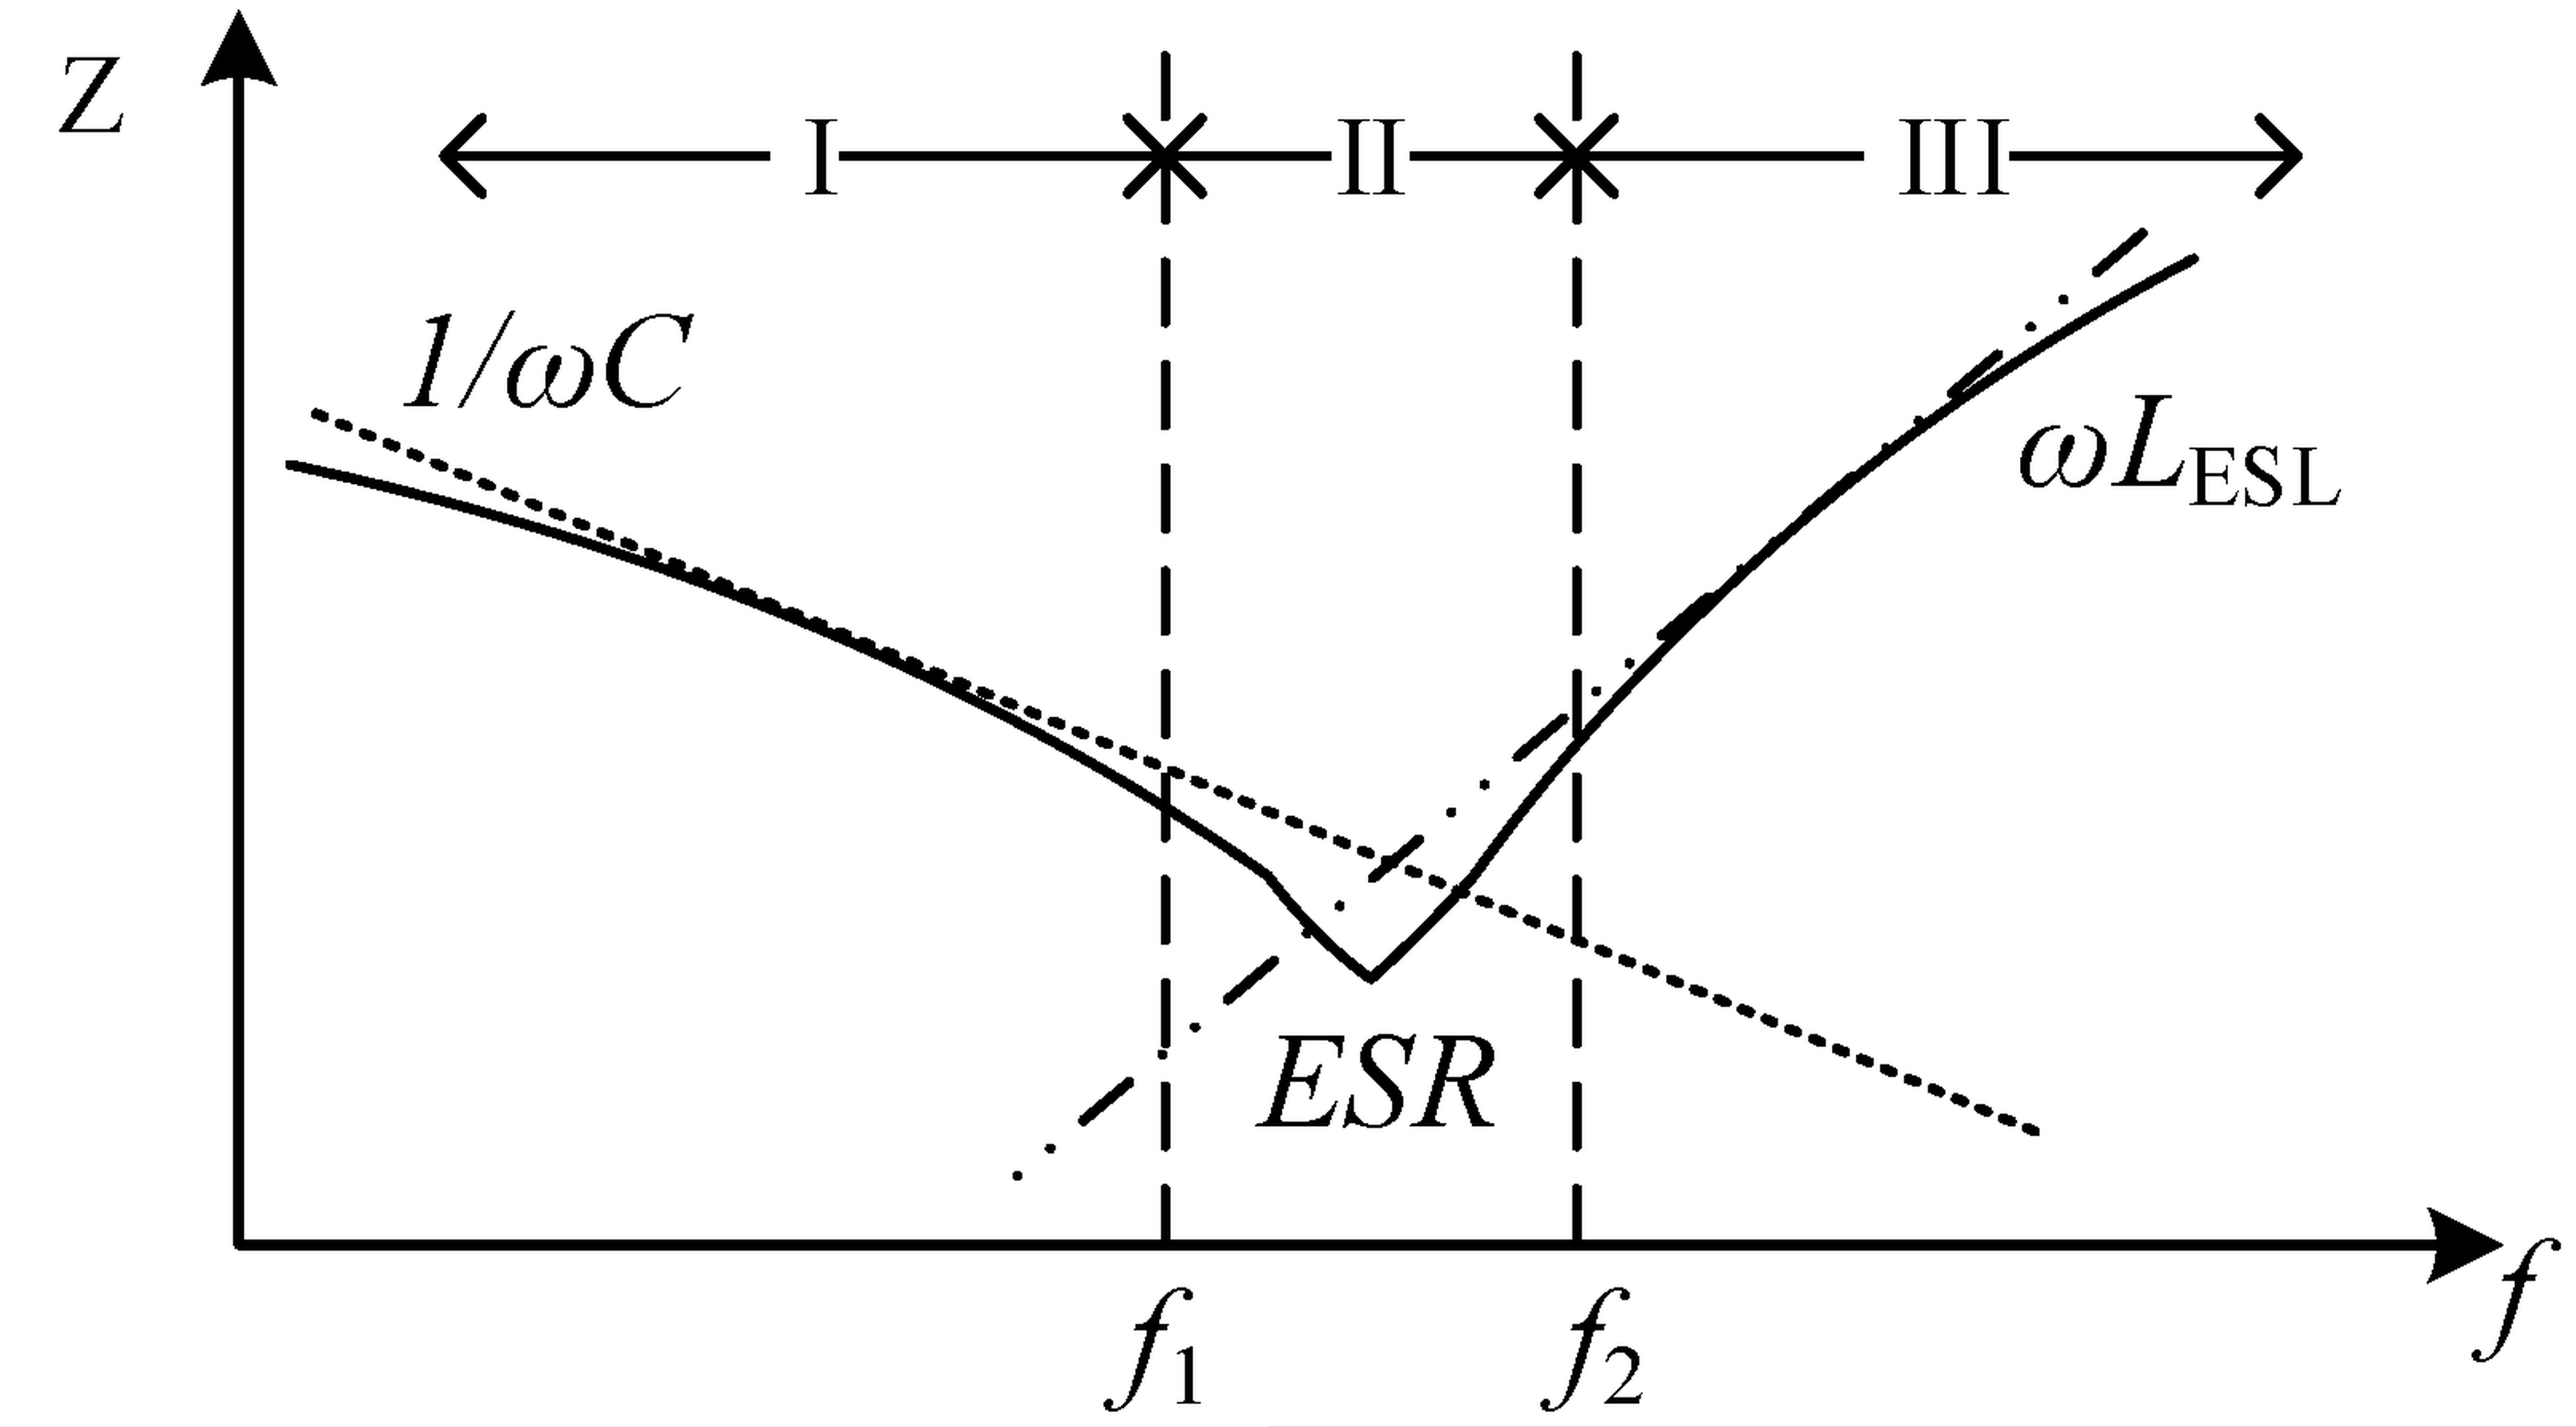
\includegraphics[width = \textwidth, height = 0.6\textwidth]{chap/04-theresa/img/esl_esr.tikz}
	\caption[Impedance response of a real capacitor]{Qualitative impedance response of a real capacitance \cite{Dang2020}}
	\label{fig:esl_esr}
\end{figure}


To deal with the low frequency variation, a large capacitor (typical values: \SIrange{10}{100}{\micro\farad}) is placed next to the component, not more than \SI{5}{\centi \metre} away.
The role of this capacitor is to be a charge supply for the instantaneous needs of the device, i.e. keeping a constant voltage level until the slower control loop of the voltage regulator can compensate for the changed current draw. \cite{decouple}
This capacitor is also called \textit{decoupling capacitor}.

Another, small capacitor (typical values: \SIrange{0.01}{0.1}{\micro \farad}) is placed as close as possible to the power pins of the component.
This capacitor should bypass (therefore also called \textit{bypass capacitor}) the high frequency variation on the power supply line. \cite{decouple}

To cover a larger frequency range, multiple capacitors can be used.

All capacitors should be connected through vias or short traces to a large area, low impedance ground plane.
vias on a \gls{pcb} are used to connect different layers, a plane is an uninterrupted area of metal covering the whole (or part) of a \gls{pcb} layer (basic \gls{pcb} structures are also  explained in \autoref{ssec:pcb_structs}). 
Connecting capacitors in this way minimizes the inductance due to connection traces. \cite{decouple}

An optional ferrite bead in series with the supply pin keeps external high frequency from the device and the noise generated inside the component from the rest of the board. \cite{decouple}


\subsection{Connectors}\label{sec:connectors}
The number and type of connectors is primarily defined by the read-out card, on which the sampling board is mounted.
The different connector types serve different purposes, which can be organized into three categories.

\paragraph{Digital Control Signals}
For digital control (i.e. \gls{spi}, enable signals, \ldots) and clocking signals a VITA 57.4 FMC+ connector from \textit{SAMTEC} is used (see \autoref{fig:fmcp}). 

\gls{fmc} is a standard defined by \gls{vita} to provide a standard mezzanine card\footnote{A \gls{pcb} which is plugged on a plug-in board. \cite{mezzanine}} form factor, connectors and modular interface to a \gls{fpga} located on a base board (carrier card). \cite{Seelam2009}
The \gls{fmc}+ standard extends the pin count and throughput of the present high-speed interfaces. 
An assembly drawing of the \gls{fmc}+ connector is shown in \autoref{fig:fmcp}.
\begin{figure}[H]
	\centering
	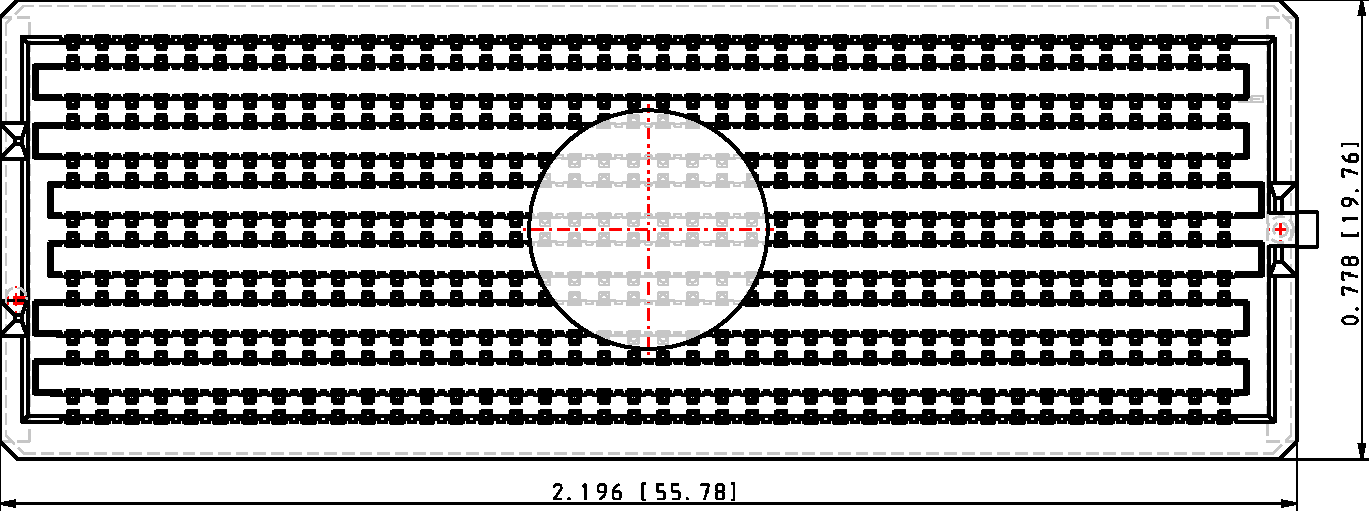
\includegraphics[width = 0.7\textwidth]{chap/04-theresa/img/connectors/fmcp.pdf}
	\caption[Rendering of FMC+ connector]{Part drawing of FMC+ connector \cite{fmcpic}}
	\label{fig:fmcp}
\end{figure}

The \gls{fmc}+ connector provides 560 pins arranged in a $14\times40$ array, 80 of which are additional high-speed interfaces, located on either side of the connector (therefore this connector type is also called \gls{hspce} connector, as opposed to the HSPC connector which has no additional rows).
For user-defined purpose 160 pins are available. 
They can be used as single-ended or differential pins.
Clocking capable pins can be used to propagate clock signals from the mezzanine to the carrier board. 

Furthermore, the connector provides pins for power supply from the carrier board to the mezzanine card. \cite{fmc} 
The voltage levels provided are listed in \autoref{tab:fmc_ps}.

\begin{table}[tb]
	\caption[FMC+ Voltages]{Voltage levels provided by the \gls{fmc}+}
	\label{tab:fmc_ps}
		\centering
		\begin{tabularx}{\textwidth}{XSS}
			\toprule
			{\textbf{Voltage}}                       & {\textbf{Max. current (\si{\ampere})}} & {\textbf{Max. capacitive load (\si{\micro\farad})}} \\ \midrule
			\SIrange{0}{3.3}{\volt} ($V_\text{ADJ}$) & 4                                      & 1000                                                \\
			\SI{3.3}{\volt}                          & 3                                      & 1000                                                \\
			\SI{12}{\volt}                           & 1                                      & 1000                                                \\ \bottomrule
		\end{tabularx}
\end{table}

\paragraph{Analog Signals}
The analog signals coming from the power-splitter are propagated to the \glspl{tha} through \SI{1.85}{\mm} high-frequency connectors. 
These connectors use an air dielectric filled interface which enables operation up to \SI{65}{\GHz}. 
This type of connector is also called ``V connector''. 
Due to its frequency range it is considered as a mm-wave \gls{rf} connector.
It is therefore used in precision instrumentation and other laboratory applications.
The design has been introduced as an open standard under the \gls{ieee} 287 Precision Connector Standards Committee. \cite{v_conn}

\autoref{fig:v_conn} shows a V connector in male and female type.
\begin{figure}[H]
	\centering
	\begin{subfigure}{0.4\textwidth}
		\centering
		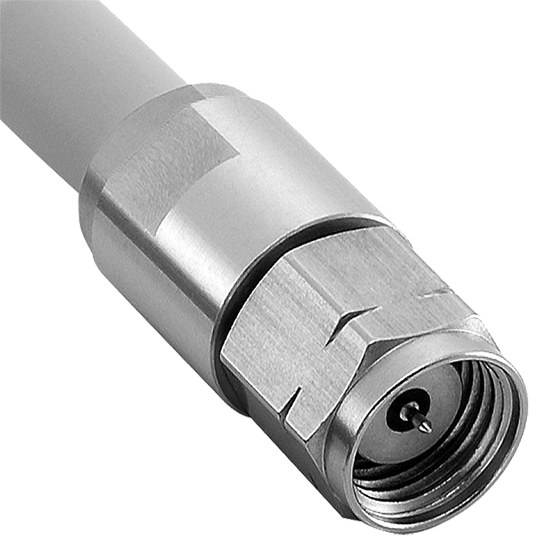
\includegraphics[width=0.7\textwidth]{chap/04-theresa/img/connectors/v_m}  
		\caption{V connector, male type}
		\label{fig:v_m}
	\end{subfigure}
	\hfill
	\begin{subfigure}{0.4\textwidth}
		\centering
		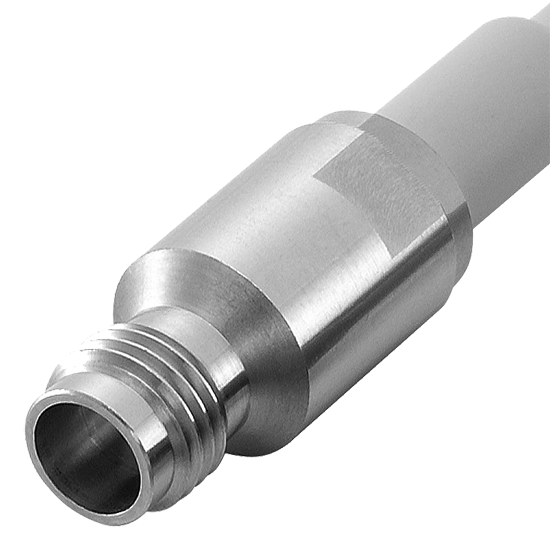
\includegraphics[height=0.7\textwidth]{chap/04-theresa/img/connectors/v_f}  
		\caption{V connector, female type}
		\label{fig:v_f}
	\end{subfigure}
	\caption{Male and female type V connector \cite{v_conn}}
	\label{fig:v_conn}
\end{figure}

On the read-out board two RFMC 2.0 (\gls{rf} Mezzanine Card) interface connectors are provided.
The connectors used are \gls{lpaf} connectors from \textit{SAMTEC} with 400 pins arranged in a $8\times50$ array.
One connector is dedicated for transmitting signals from the mezzanine card to the on-board \glspl{adc}.
The other provides the analog output from the on-board \glspl{dac}\footnote{A \gls{dac} translates digital values into an analog signal.} to the mezzanine card.
On the sampling board, the male counterpart of the connectors, \gls{lpam}, is used (see \autoref{fig:lpam1}).

\begin{figure}[tb]
	\centering
	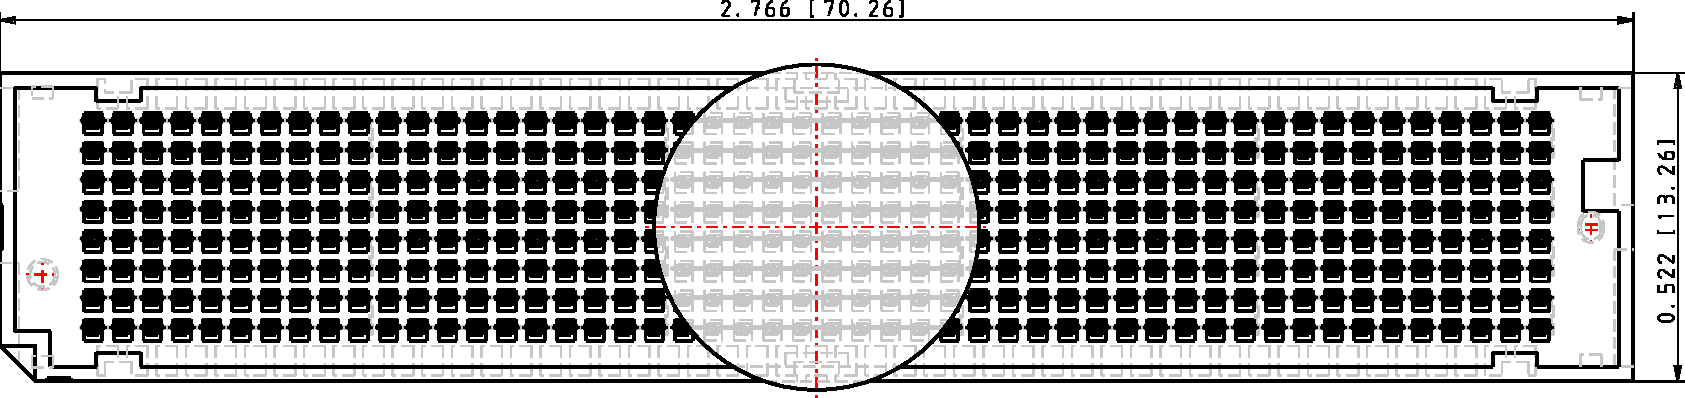
\includegraphics[width = \textwidth]{chap/04-theresa/img/connectors/lpam_50_top.pdf}
	\caption[LPAM $8\times50$ connector]{Part drawing of a LPAM $8\times50$ connector}
	\label{fig:lpam1}
\end{figure}


\paragraph{Clock Signals}
The clock signals from the \glspl{pll} on the sampling board are propagated in different ways.
The reference clock for the \gls{fpga} is propagated through the \gls{fmc}+ connector.
Clocking for the \glspl{adc} and the \glspl{dac} is provided through a $6\times20$ \gls{lpam} connector (see \autoref{fig:lpam2}).
\begin{figure}[tb]
	\centering
	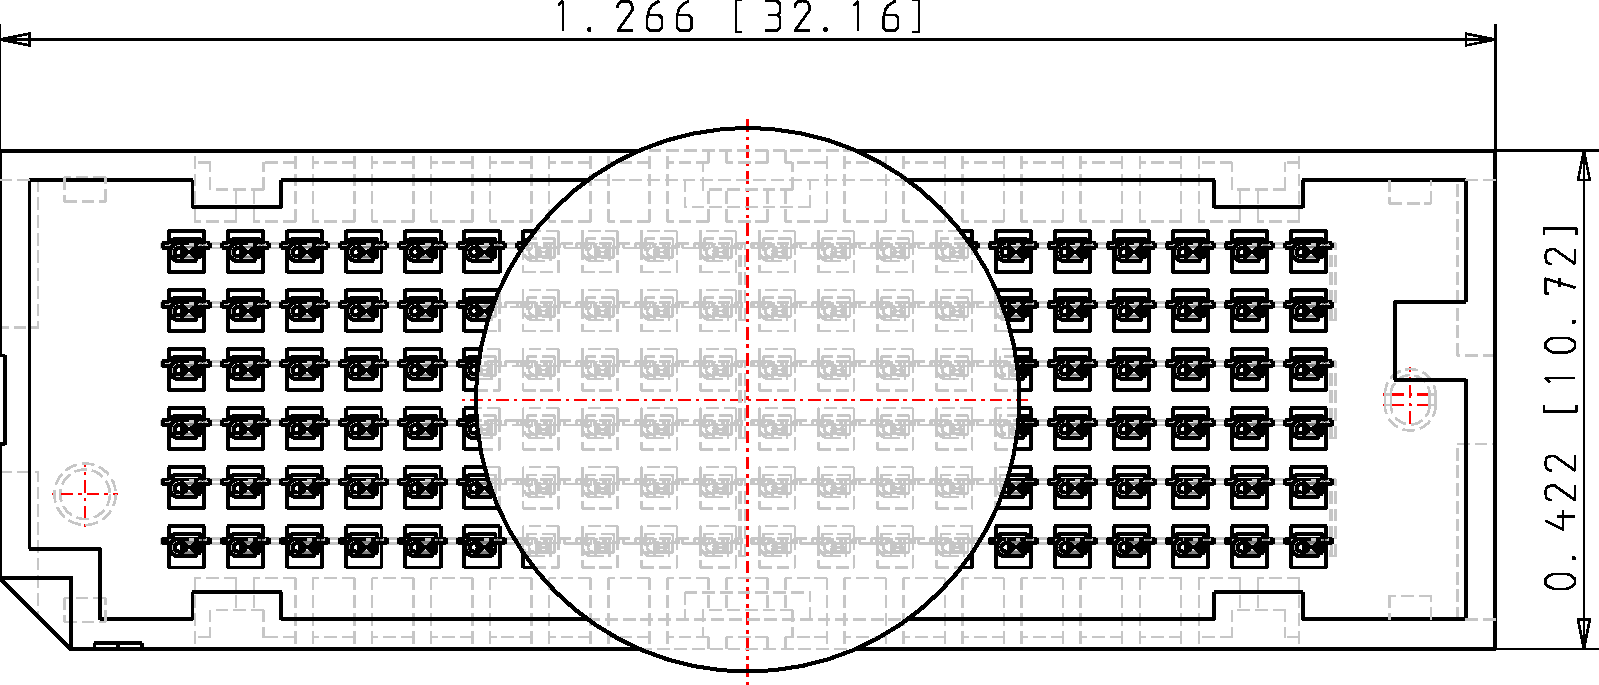
\includegraphics[width = 0.7\textwidth]{chap/04-theresa/img/connectors/lpam_20.pdf}
	\caption[LPAM $6\times20$ connector]{Part drawing of LPAM $6\times20$ connector}
	\label{fig:lpam2}
\end{figure}

The clock coming from \gls{kara} is provided through \gls{rf} SMA connectors directly to the \gls{pll}.

\subsection{Sampling-Channel}
The most important circuit part of the sampling board is the sampling channel. 
On the board, 16 of such sampling channels are present integrating a wide-band \gls{tha} and delay chip.
The sampling time of the \gls{tha}, derived from the clock coming from the main \gls{pll} on the board, can be delayed individually by programming the delay time of each delay chip respectively (via \gls{fpga}). 

\subsubsection*{Track-And-Hold-Amplifier}
The \gls{tha} used is the same as in \gls{kapture}. 
The component was chosen due to its high bandwidth (> \SI{18}{\GHz}) and low aperture jitter (range of hundreds of femtoseconds). \cite{caselle2013} 
Therefore it is also a good candidate for the new \gls{theresa} sampling board.

The main features of the \gls{tha} are listed in \autoref{tab:hmc5640}.
These input specifications are important for the later interface with the \gls{adc} with the delay chip.
Switching characteristics are important for estimation of the maximal sample frequency possible and overall performance of the system.
\begin{table}[tb]
	\caption[HMC5640 Characteristics]{Specifications of the HMC5640 \gls{tha}}
	\label{tab:hmc5640}
	\begin{minipage}{\textwidth}
		\centering
		\begin{tabularx}{\textwidth}{Xcccc}
			\toprule
			\textbf{Parameter} & \textbf{Min} & \textbf{Typ.} & \textbf{Max} & \textbf{Unit}\\
			\midrule
			\multicolumn{5}{c}{\textbf{Analog Inputs}}  \\
			Differential \gls{fs} Range & & 1 & & Vpp\footnote{Volt peak-to-peak}\\
			Common mode voltage & -0.1 & 0 & 0.1 & V\\[0.3cm]
		    \multicolumn{5}{c}{\textbf{Clock Inputs}}  \\
			DC Differential High Voltage (Track Mode) & 20 & 40 & 2000 & mV\\
			DC Differential Low Voltage (Hold Mode) & -2000 & -40 & -20 & mV\\
			Common mode voltage & -0.5 & 0 & 0.5 & V\\[0.3cm]
		    \multicolumn{5}{c}{\textbf{Analog Outputs}}  \\
			Differential \gls{fs} Range &  & 1 && Vpp\\
			Common mode voltage & & 0 & & V\\[0.3cm]
			\multicolumn{5}{c}{\textbf{Track-to-Hold/Hold-to-Track Switching}} \\
			Aperture Delay & & -6 &  & ps\\
			Random Aperture Jitter (\gls{fs}, \SI{1}{\giga \hertz}) & & < 70 & & fs\\
			Settling time\footnote{\textit{Settling time} is the interval between the internal track-hold transition and the time when the output signal is settled within the specified value.} (to \SI{1}{\milli \volt}) &	&  116 & & ps \\
			\bottomrule
		\end{tabularx}
	\end{minipage}
\end{table}

The input coming from the power-splitter is single-ended.
However, the analog input of the \gls{tha} is differential, therefore a \SI{50}{\ohm} termination on the unused input pin has been added, as recommended in the data sheet \cite{hmc5640}.

The differential outputs are connected to the corresponding RFMC \gls{lpam} 8$\times$50 connector pins.
The schematics of the \gls{tha} is shown in \autoref{fig:hmc5640}.

At the power pins, \gls{rf} filters containing decoupling capacitors and ferrite beads are placed. The \gls{tha} is a crucial component, as it samples the sensor signal, therefore any possible noise should be reduced to a minimum by proper filtering.

\begin{figure}[tb]
	\centering
	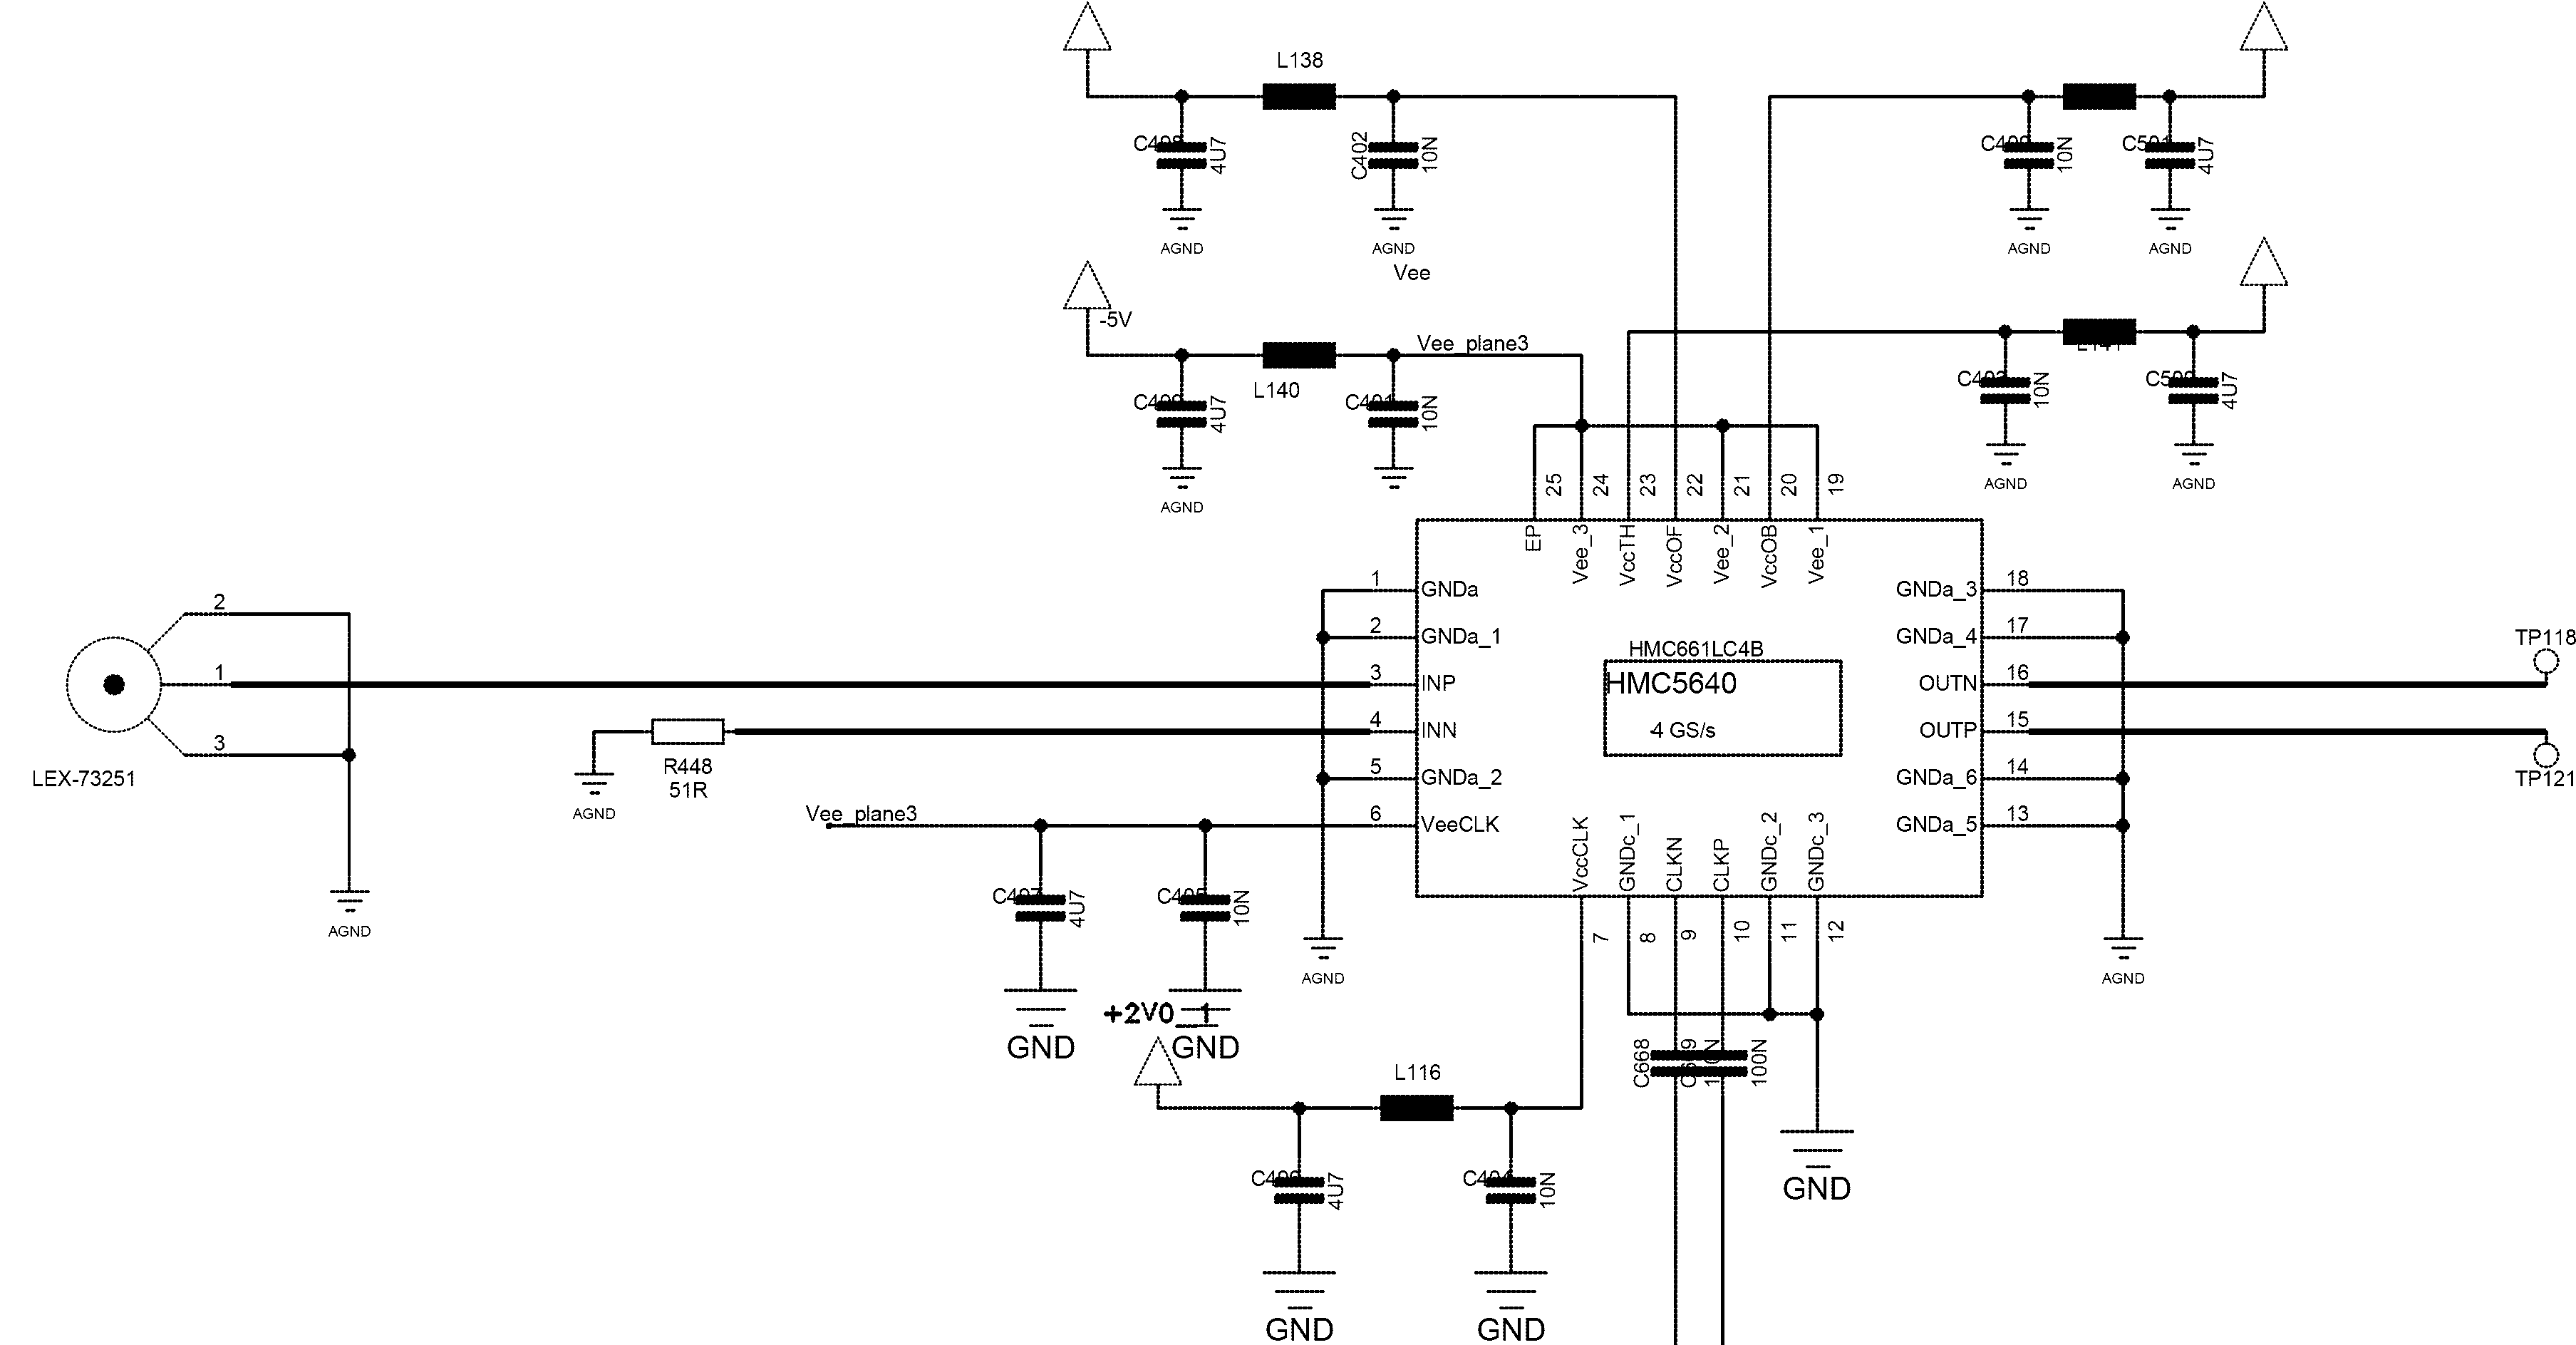
\includegraphics[width = \textwidth]{chap/04-theresa/img/schematic/hmc5640}
	\caption[HMC5640 THA schematic]{HMC5640 \gls{tha} schematic}
	\label{fig:hmc5640}
\end{figure}
\clearpage
\paragraph{Separating Analog and Digital Ground}
Digital grounds are more noisy than analog grounds due to switching events of the digital components. 
Analog components are more sensitive to noise (due to e.g. lower signal amplitudes) than digital components\footnote{Digital components work with voltage thresholds, rather than continuous voltage levels.} and need a clean ground.
In a mixed-signal (having both analog and digital signals) \gls{pcb}, analog and digital ground should therefore be well separated.
For some mixed-signal components, such as \glspl{tha}, where separate analog and digital ground pins are provided, it is however recommended to connect both grounds directly at the component.
For the \glspl{tha} in this design, this is done by connecting the ground pins via ferrite bead at each \gls{tha} (see \autoref{fig:gnd_agnd}). 
The ferrite bead mitigates any high-frequency components and therefore protects the analog ground from noise. %todo components?
For every \gls{tha}, one ferrite bead is needed, making a total of 16 beads (see \autoref{fig:gnd_agnd}).

Protection against possible high voltage levels between analog and digital grounds is implemented by two back-to-back diodes \autoref{fig:gnd_agnd}).
The diodes should limit this voltage to around \SI{0.6}{\volt}.

\begin{figure}[tb]
	\centering
	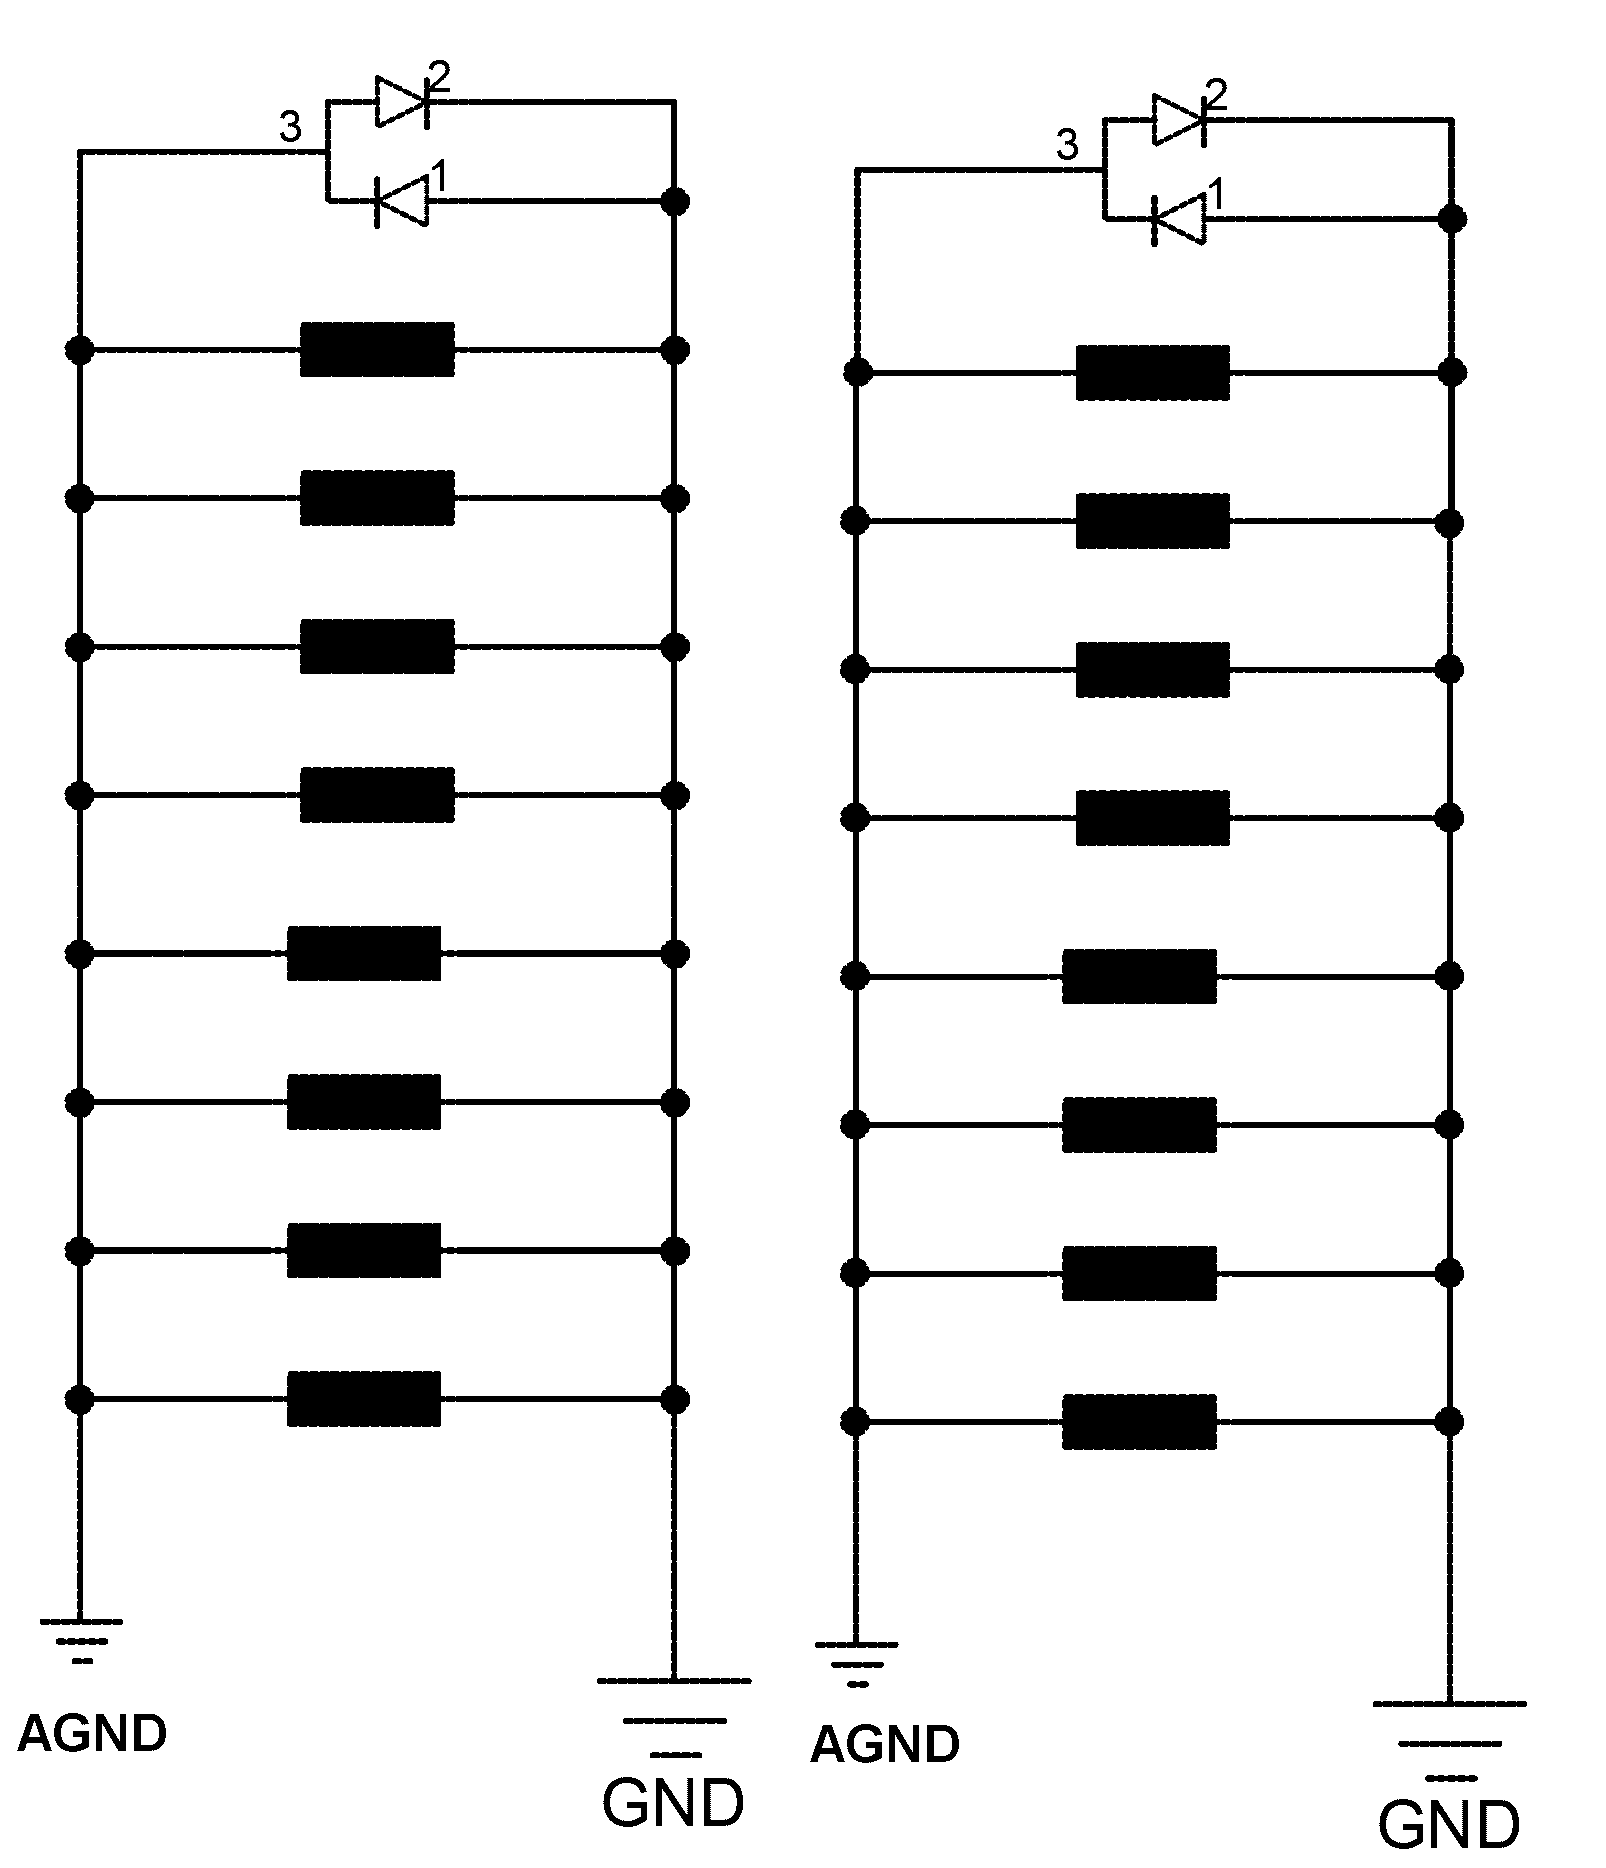
\includegraphics[width = 0.5\textwidth]{chap/04-theresa/img/schematic/gnd_agnd}
	\caption{Connection of the analog and digital grounds at the THAs}
	\label{fig:gnd_agnd}
\end{figure}

\subsubsection*{Delay Chip}
The delay chips are used to create a delay in the sampling time of the \gls{tha} chips. For the selection of the delay chip, the most important characteristics, apart from time jitter, is the delay step size and delay range. 

To optimize the performance of \gls{theresa} and allowing a sample rate up to \SI{40}{\giga\sample\per\second} (see \autoref{ssec:interl_impl}), the step-size of the delay chip must not exceed \SI{25}{\pico \second}.

With the HMC856 delay chip from \textit{Analog Devices}, which is also used for the \gls{kapture} sampling board, a minimal step size of \SI{3}{\pico\second} (see \cite{hmc856}) is possible.
This is much less than  \SI{25}{\pico \second} and thus the chip could be potentially used for the intended purpose.
However, one drawback is the limited delay range of \SI{100}{\pico\second}.
Considering a signal, which is stretched over several nanoseconds, this range limits the possibility to sample time-stretched pulses.
Another challenge, coming from the available number of I/Os, is the programming interface of the chip which consists of five differential \gls{cml} inputs.
This means, one chip already takes up 10 pins only for control signals.
For a total of 16 necessary delay chips, this results in 160 pins used only for control of the delay chips.
This uses up all pins of the \gls{fmc}+ connector (see \autoref{sec:connectors}) available for user-defined purpose. 

A better candidate is the dual channel programmable delay chip NB6L295 from \textit{ON Semiconductor}. 
This chip provides two separately programmable delay channels. 
This reduces the necessary chip count by half and therefore reduces the overall complexity of the \gls{pcb}.
The minimal delay step size of \SI{11}{\pico\second} lies under the maximal allowed \SI{25}{\pico \second}. Therefore the chip is suitable for the targeted interleaving method, covering a total delay range up to \SI{8.8}{\nano\second} per delay channel.
This enables the covering of the whole time-stretched signal, the duration of which lies in the range of nanoseconds.
The chip is programmed via \gls{sdi} (see \cite{NB6L295}), which only requires 4 pins (enable pin, data pin, clock pin, load pin). 
Thus, the total number of digital control pins used by the delay chips is $4\cdot8 = 32$, which is a significant reduction compared to the 160 control pins needed by the HMC856 chips. 
This number can be even more reduced, by propagating the same data, clock and load pins to the chips and providing the enable signal on individual lines to the respective chip (see \autoref{fig:delay_sdi}). 
In this way, only 11 pins (8 enable pins and 3 pins for data, clock and load) are necessary in total for programming all delay chips. 

\begin{figure}[tb]
	\centering
	%\includegraphics[scale=0.5]{chap/04-theresa/img/delay_sdi}
	\resizebox{1\textwidth}{!}{  \tikzset{myblock/.style = {rectangle, draw, minimum width=3cm, minimum height = 3cm}}
	 %, minimum width=3cm, minimum height = 3cm
\begin{tikzpicture}%[scale=0.6, every node/.style={scale=0.6}]
	    \node (c1)[myblock]{\Large Chip 1};
	\begin{scope}[shift={(4,0)}]
		\node (c2)[myblock] {\Large  Chip 2};
	\end{scope}
	\begin{scope}[shift={(8,0)}]
		\node (c3)[myblock]{\Large  Chip 3};
	\end{scope}
	\begin{scope}[shift={(12,0)}]
		\node (c4)[myblock]{\Large  Chip 4};
	\end{scope}
	\begin{scope}[shift={(16,0)}]
		\node (c5)[myblock]{\Large  Chip 5};
	\end{scope}
	\begin{scope}[shift={(20,0)}]
		\node (c6)[myblock]{\Large  Chip 6};
	\end{scope}
	\begin{scope}[shift={(24,0)}]
		\node (c7)[myblock]{\Large  Chip 7};
	\end{scope}
	\begin{scope}[shift={(28,0)}]
		\node (c8)[myblock]{\Large  Chip 8};
	\end{scope}

	\draw[-Latex] (-3,3) node[left] {\Huge \texttt{SLOAD}} -| coordinate (1)  ($(c1.north west)!0.2!(c1.north east)$) ;
	\draw[-Latex] (-3,3) -| coordinate (2)  ($(c2.north west)!0.2!(c2.north east)$) ;
	\draw[-Latex] (-3,3) -| coordinate (3)  ($(c3.north west)!0.2!(c3.north east)$) ;
	\draw[-Latex] (-3,3) -| coordinate (4)  ($(c4.north west)!0.2!(c4.north east)$) ;
	\draw[-Latex] (-3,3) -| coordinate (5)  ($(c5.north west)!0.2!(c5.north east)$) ;
	\draw[-Latex] (-3,3) -| coordinate (6)  ($(c6.north west)!0.2!(c6.north east)$) ;
	\draw[-Latex] (-3,3) -| coordinate (7)  ($(c7.north west)!0.2!(c7.north east)$) ;
	\draw[-Latex] (-3,3) -| coordinate (8)  ($(c8.north west)!0.2!(c8.north east)$) ;

	\draw[-Latex] (-3,4) node[left] {\Huge \texttt{SCLK}} -|  coordinate (9) ($(c1.north west)!0.4!(c1.north east)$) ;
	\draw[-Latex] (-3,4) -| coordinate (10) ($(c2.north west)!0.4!(c2.north east)$) ;
	\draw[-Latex] (-3,4) -| coordinate (11) ($(c3.north west)!0.4!(c3.north east)$) ;
	\draw[-Latex] (-3,4) -| coordinate (12) ($(c4.north west)!0.4!(c4.north east)$) ;
	\draw[-Latex] (-3,4) -| coordinate (13) ($(c5.north west)!0.4!(c5.north east)$) ;
	\draw[-Latex] (-3,4) -| coordinate (14) ($(c6.north west)!0.4!(c6.north east)$) ;
	\draw[-Latex] (-3,4) -| coordinate (15) ($(c7.north west)!0.4!(c7.north east)$) ;
	\draw[-Latex] (-3,4) -| coordinate (16) ($(c8.north west)!0.4!(c8.north east)$) ;

	\draw[-Latex] (-3,5) node[left] {\Huge \texttt{SDIN}} -| coordinate (17) ($(c1.north west)!0.6!(c1.north east)$) ;
	\draw[-Latex] (-3,5) -| coordinate (18) ($(c2.north west)!0.6!(c2.north east)$) ;
	\draw[-Latex] (-3,5) -| coordinate (19) ($(c3.north west)!0.6!(c3.north east)$) ;
	\draw[-Latex] (-3,5) -| coordinate (20) ($(c4.north west)!0.6!(c4.north east)$) ;
	\draw[-Latex] (-3,5) -| coordinate (21) ($(c5.north west)!0.6!(c5.north east)$) ;
	\draw[-Latex] (-3,5) -| coordinate (22) ($(c6.north west)!0.6!(c6.north east)$) ;
	\draw[-Latex] (-3,5) -| coordinate (23) ($(c7.north west)!0.6!(c7.north east)$) ;
	\draw[-Latex] (-3,5) -| ($(c8.north west)!0.6!(c8.north east)$) ;

	\draw[Latex-]  ($(c1.north west)!0.8!(c1.north east)$) --  ++(0,5) node[above] {\Huge \texttt{EN}$_1$}; 
	\draw[Latex-]  ($(c2.north west)!0.8!(c2.north east)$) --  ++(0,5) node[above] {\Huge EN2}; 
	\draw[Latex-]  ($(c3.north west)!0.8!(c3.north east)$) --  ++(0,5) node[above] {\Huge EN3}; 
	\draw[Latex-]  ($(c4.north west)!0.8!(c4.north east)$) --  ++(0,5) node[above] {\Huge EN4}; 
	\draw[Latex-]  ($(c5.north west)!0.8!(c5.north east)$) --  ++(0,5) node[above] {\Huge EN5}; 
	\draw[Latex-]  ($(c6.north west)!0.8!(c6.north east)$) --  ++(0,5) node[above] {\Huge EN6}; 
	\draw[Latex-]  ($(c7.north west)!0.8!(c7.north east)$) --  ++(0,5) node[above] {\Huge EN7}; 
	\draw[Latex-]  ($(c8.north west)!0.8!(c8.north east)$) --  ++(0,5) node[above] {\Huge EN8}; 


	\filldraw[black] (1) circle (2pt); 
	\filldraw[black] (2) circle (2pt); 
	\filldraw[black] (3) circle (2pt); 
	\filldraw[black] (4) circle (2pt); 
	\filldraw[black] (5) circle (2pt); 
	\filldraw[black] (6) circle (2pt); 
	\filldraw[black] (7) circle (2pt); 
	\filldraw[black] (9) circle (2pt); 
	\filldraw[black] (10) circle (2pt); 
	\filldraw[black] (11) circle (2pt); 
	\filldraw[black] (12) circle (2pt); 
	\filldraw[black] (13) circle (2pt); 
	\filldraw[black] (14) circle (2pt); 
	\filldraw[black] (15) circle (2pt); 
	\filldraw[black] (17) circle (2pt); 
	\filldraw[black] (18) circle (2pt); 
	\filldraw[black] (19) circle (2pt); 
	\filldraw[black] (20) circle (2pt); 
	\filldraw[black] (21) circle (2pt); 
	\filldraw[black] (22) circle (2pt); 
	\filldraw[black] (23) circle (2pt);
\end{tikzpicture}}
	\caption[Delay chip SDI connections]{Diagram of the SDI control pins for the NB6L295 delay chip. The data (\texttt{SDIN}), clock (\texttt{SCLK}) and load (\texttt{SLOAD}) pins are shared by all chips. Only the enable (\texttt{EN}$_x$) signals are routed individually.}
	\label{fig:delay_sdi}
\end{figure}

The schematic of the delay chips is shown in \autoref{fig:nb6l295}.

\begin{figure}[tb]
	\centering
	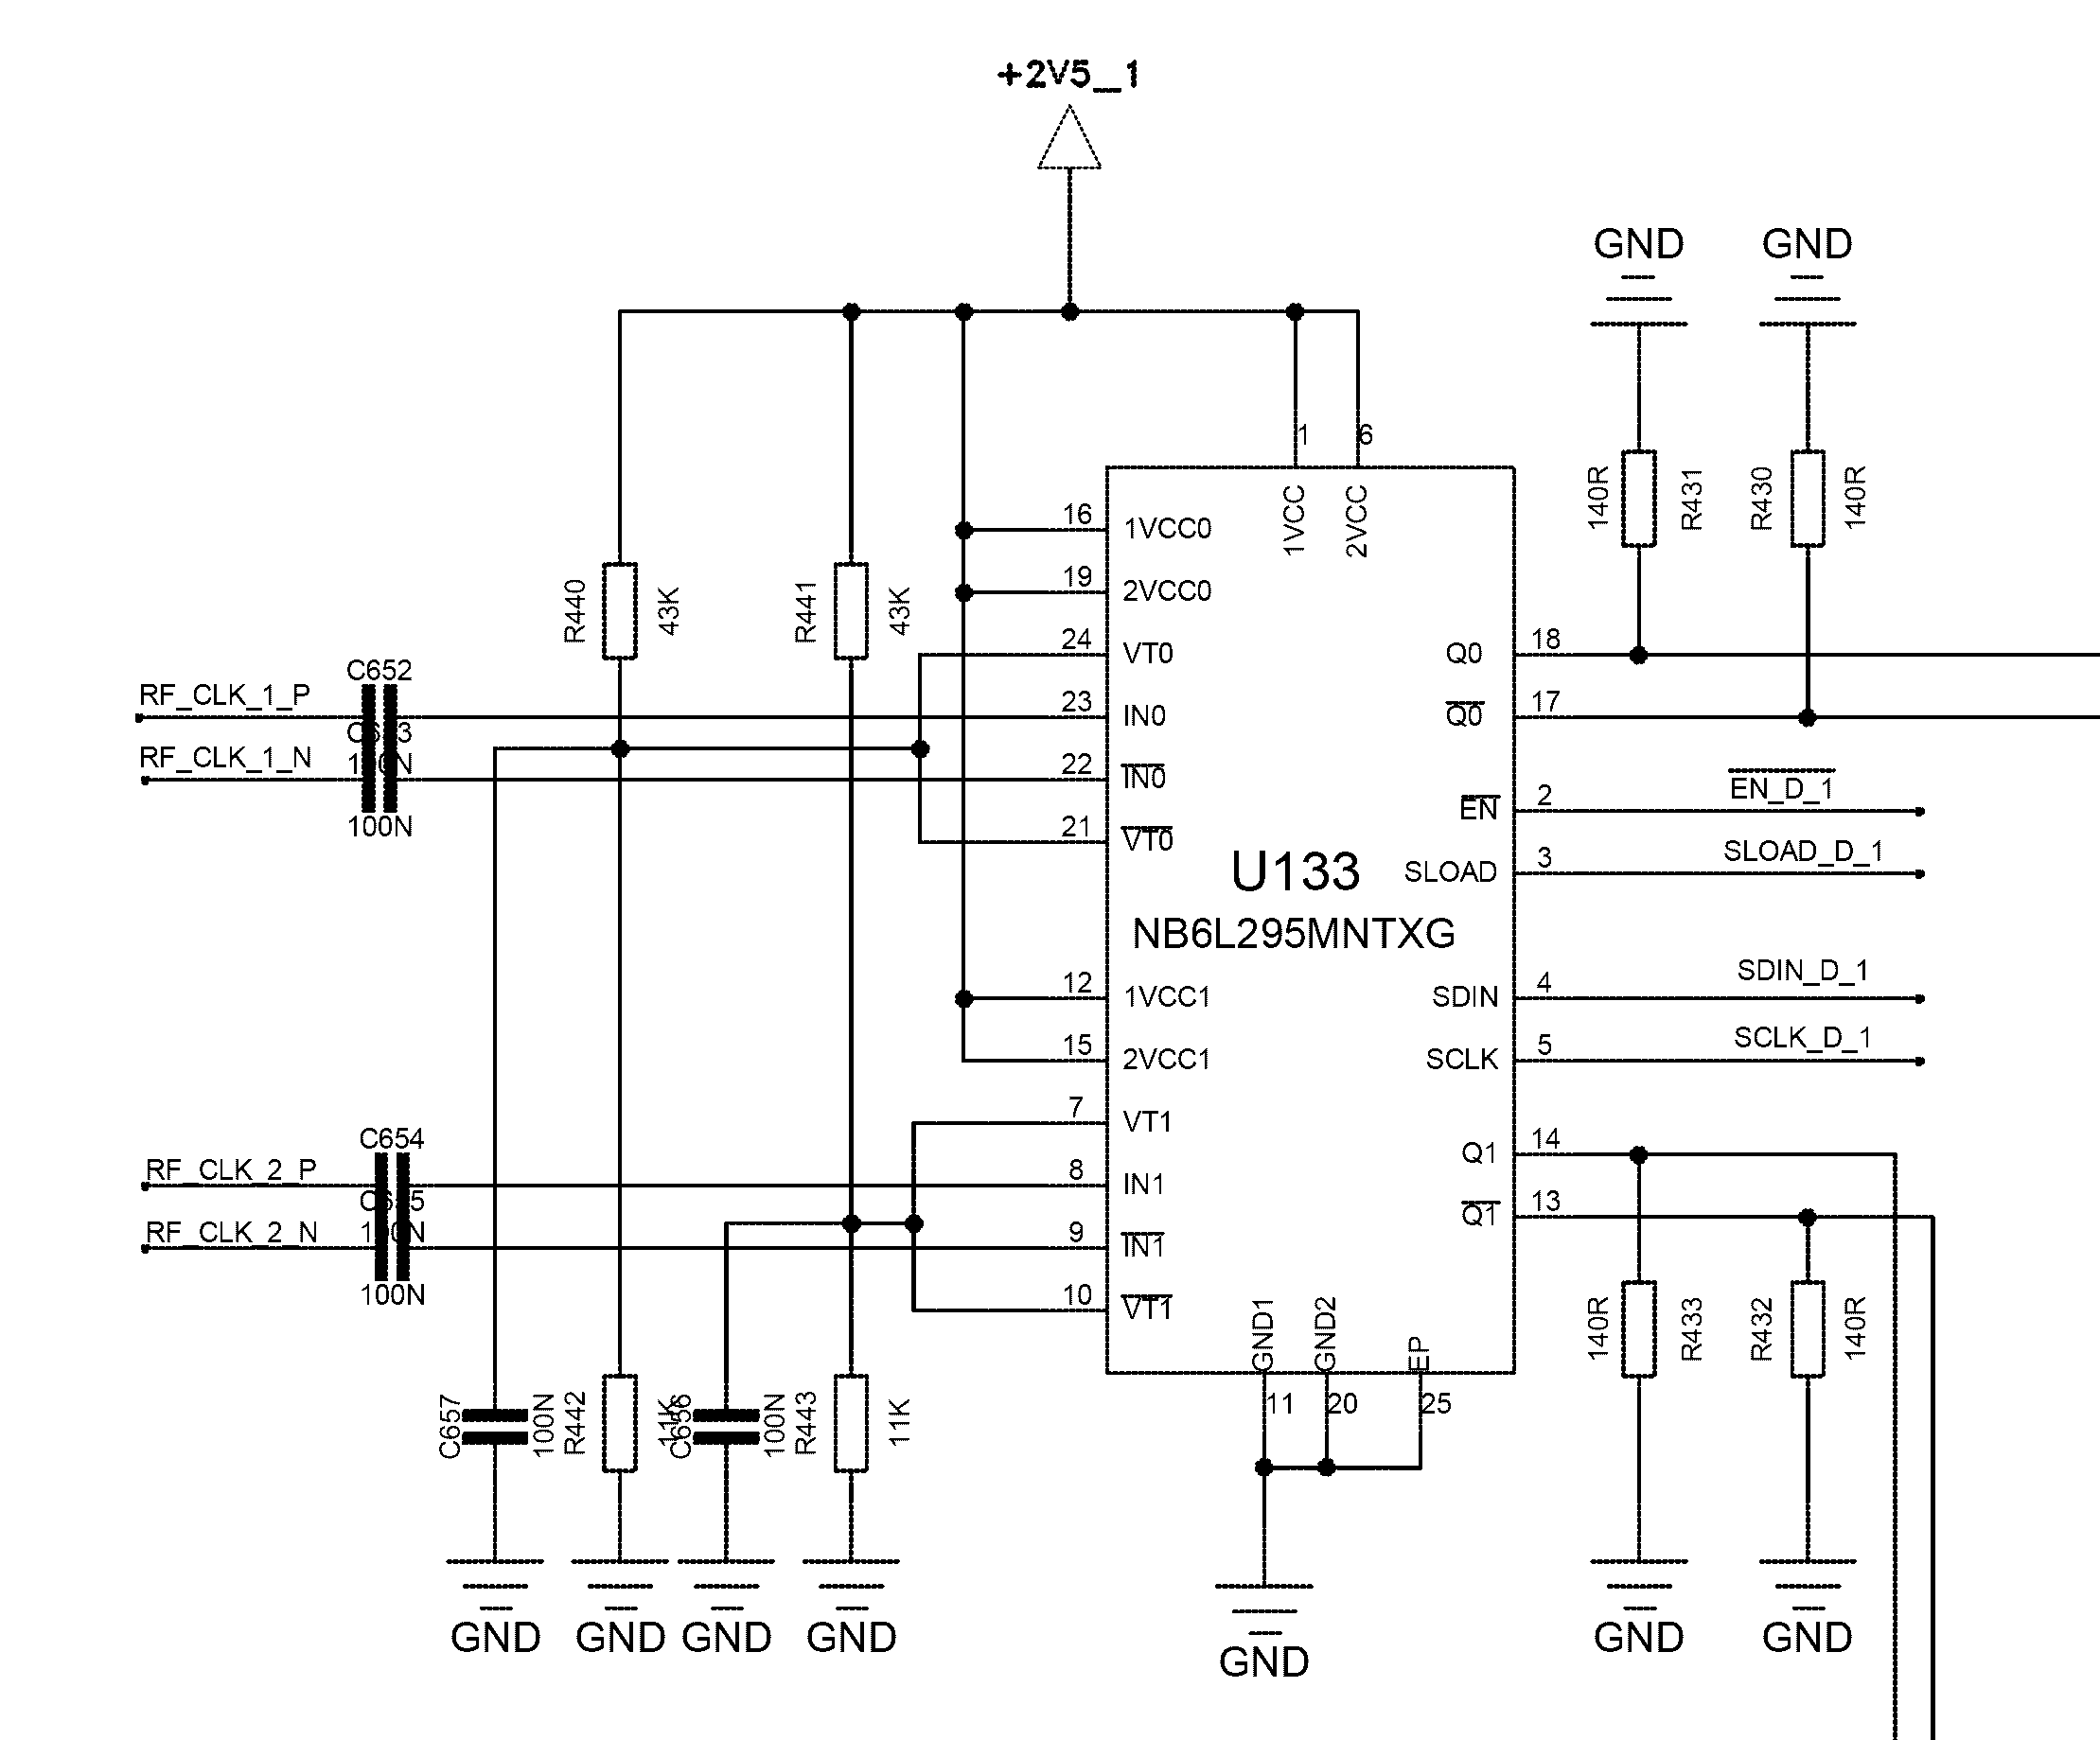
\includegraphics[width = \textwidth]{chap/04-theresa/img/schematic/delay_chip}
	\caption{NB6L295 delay chip schematic}
	\label{fig:nb6l295}
\end{figure}
%todo to texttt


\paragraph{Inputs}
The inputs of the delay chip are driven by the preceding low time-skew, low-jitter and high-performance clock distribution, the outputs of which are \gls{lvpecl} drivers.
According to the data sheet (\cite{NB6L295}), when driving the inputs with a \gls{lvpecl} driver, the VTx and $\overline{\text{VTx}}$ pins of the delay chip need to be connected to $V_\text{cc} - \SI{2}{\volt}$ (see \autoref{fig:delay_lvpecl}).
In case of $V_\text{cc}$ = \SI{2.5}{\volt}, this results in a voltage level of VTx = $\overline{\text{VTx}}$ = \SI{0.5}{\volt}.

This voltage level is achieved by using a resistive voltage divider connected to $V_\text{cc}$. 
A voltage divider with the resistors $R_1$ and $R_2$ (see \autoref{fig:v_divider}) produces a voltage $V_\text{out}$ which is a fraction of the input voltage $V_\text{in}$.
$V_\text{out}$ is calculated as
\begin{equation}\label{eq:vdiv}
	V_\text{out} = \frac{R_2}{R_1 + R_2} V_\text{in}.
\end{equation}
\begin{figure}[tb]
	\centering
	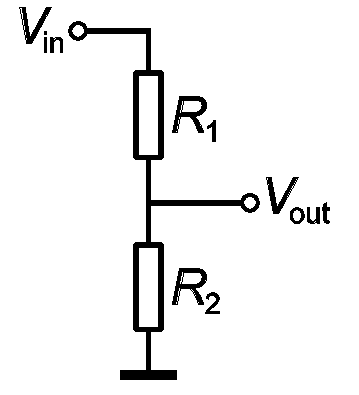
\includegraphics[height = 0.5\textwidth]{chap/04-theresa/img/voltage_divider.tikz}
	\caption{Schematic of a resistive voltage divider}
	\label{fig:v_divider}
\end{figure}
The resistor values are chosen to be $R_1 = \SI{43}{\kilo\ohm}$ and $R_2 = \SI{11}{\kilo\ohm}$.
According to \autoref{eq:vdiv} this results in a voltage of
\begin{equation}
	V_\text{cc} \frac{\SI{11}{\kilo\ohm}}{\SI{11}{\kilo\ohm} + \SI{43}{\kilo\ohm}} = \SI{0.5093}{\volt} \approx \SI{0.5}{\volt}
\end{equation}
at the VTx and $\overline{\text{VTx}}$ pins.
Resistor values are chosen high to minimize current flow.
A \SI{100}{\nano\farad} capacitor is put in parallel to stabilize $V_\text{cc}$.

\begin{figure}[tb]
	\centering
	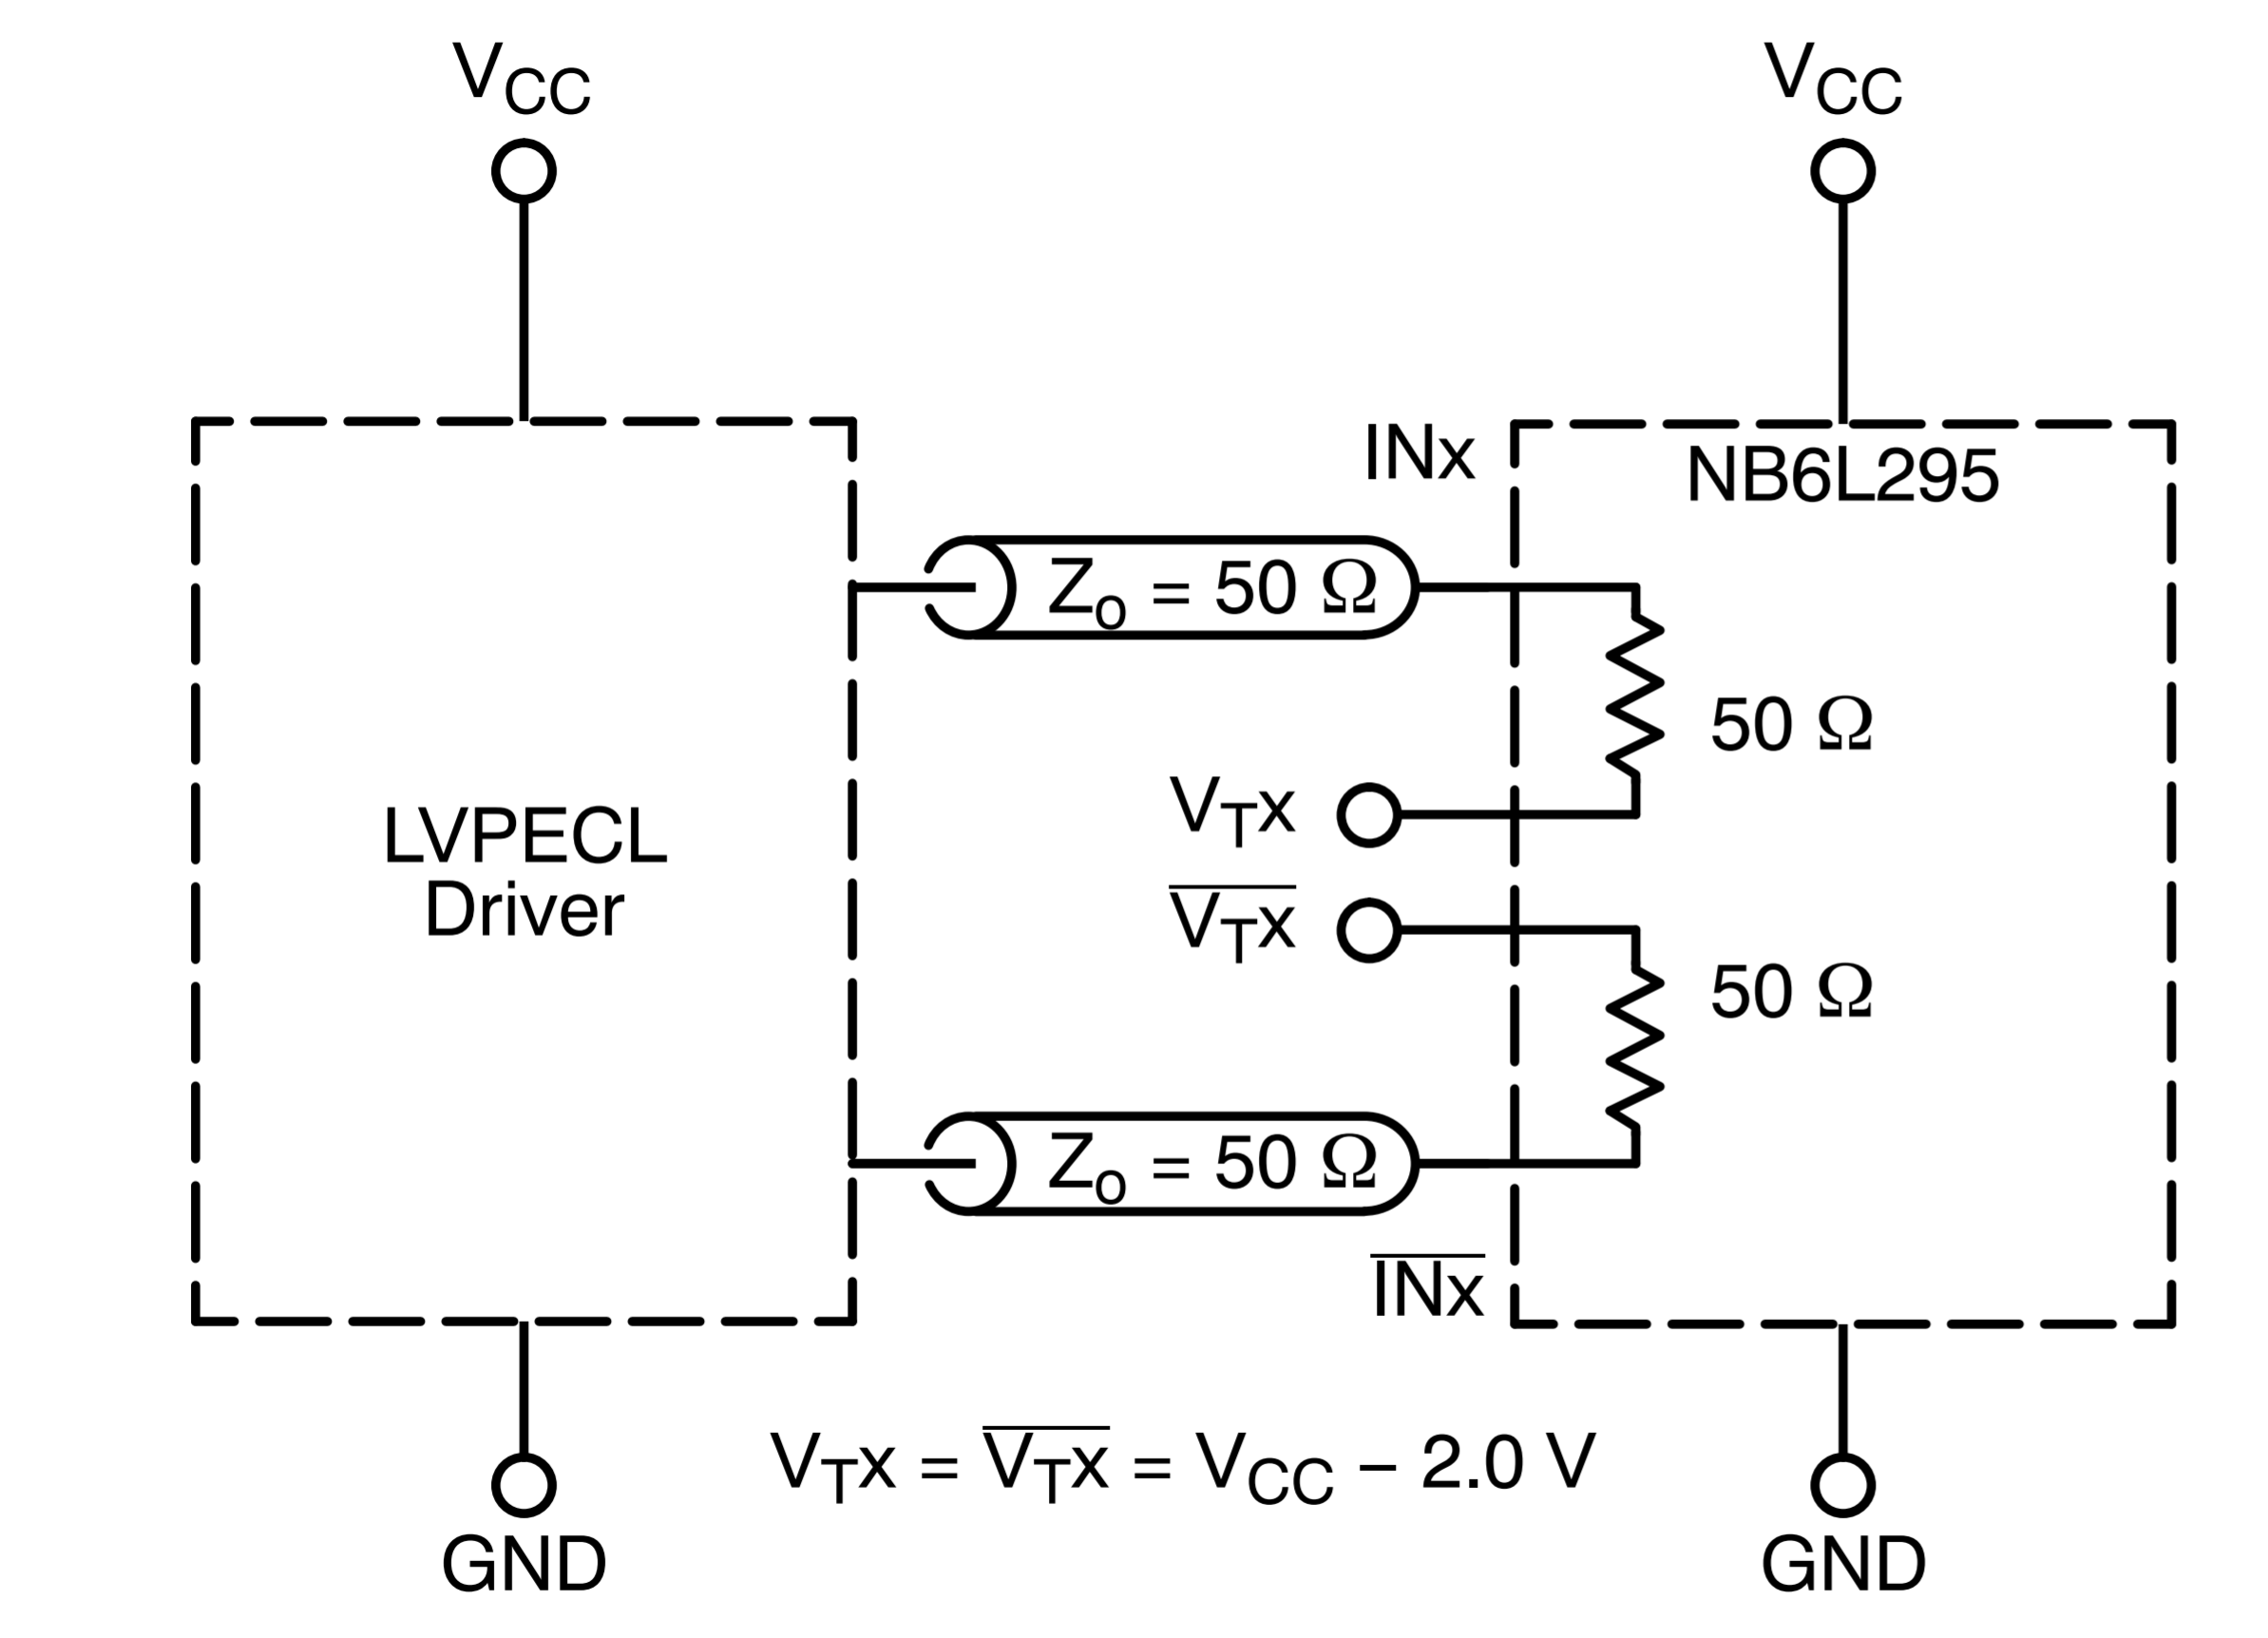
\includegraphics[width = 0.7\textwidth]{chap/04-theresa/img/delay_lvpecl}
	\caption[NB6L295 Delay Chip Schematic]{LVPECL recommendations for NB6L295 \cite{NB6L295}}
	\label{fig:delay_lvpecl}
\end{figure}


\begin{table}[tb]
	\caption[NB6L295 Characteristics]{Specifications of the NB6L295 delay chip \cite{NB6L295}}
	\label{tab:nb6l295}
	\begin{minipage}{\textwidth}
		\centering
		\begin{tabularx}{\textwidth}{Xcccc}
			\toprule
			\textbf{Parameter} & \textbf{Min} & \textbf{Typ.} & \textbf{Max} & \textbf{Unit}\\
			\midrule
			\multicolumn{5}{c}{\textbf{Outputs}}  \\
			Output HIGH Voltage & $V_\text{cc} - 1075$ & $V_\text{cc} - 950$ & $V_\text{cc} - 825$ & mV\\
			Output LOW Voltage & $V_\text{cc} - 1825$ & $V_\text{cc} - 1725$ & $V_\text{cc} - 1625$ & mV\\
			Output HIGH Voltage ($V_\text{cc}=\SI{3.3}{\volt}$) & $2225$ & $2350$ & $2475$ & mV\\
			Output LOW Voltage ($V_\text{cc}=\SI{3.3}{\volt}$) & $1475$ & $1575$ & $1675$ & mV\\
			Common mode voltage & -0.1 & 0 & 0.1 & V\\[0.3cm]
			\multicolumn{5}{c}{\textbf{AC Characteristics}}  \\
			Random Clock Jitter \gls{rms}&  & 3 & 10 & ps\\
			Output Rise/Fall Times \footnote{@\SI{50}{\mega \hertz}} & 85 & 120 & 170 & ps\\
			Serial Clock Input Frequency \footnote{50\% Duty Cycle,Percentage of the ratio of pulse width and total period of the waveform.} &  &  & 20 & MHz\\
			Minimum Pulse width SLOAD  & 1 &  &  & ns\\
			\bottomrule
		\end{tabularx}
	\end{minipage}
\end{table}
According to the data sheet \cite{NB6L295}, the digital control pins need a minimum input HIGH voltage of \SI{2}{\volt}.
Directly connecting to the \gls{fmc}+ connector pins is therefore not possible, as the maximal level provided by the readout card is smaller than \SI{2}{\volt}.
Therefore, the SN74AVC32T245 bus transceiver from \textit{Texas Instruments}, which allows for shifting the level the device input to the device output, is used. 
The schematic of the transceiver is shown in \autoref{fig:level_trans}.
In this design, the bus transceiver is configured to propagate signals from the ``A'' ports (coming from the \gls{fmc}+ connector) to the ``B'' ports (going to the delay chips), shifting the signals from the $V_\text{ADJ}$ (\SI{1.8}{\volt}) of the \gls{fmc}+ connector to \SI{2.5}{\volt} (see \autoref{fig:level_trans}).
To guarantee signal integrity and to decouple the components, the digital signals are propagated in a ``fanout configuration'', i.e. one digital signal at the input is propagated to eight outputs.
Furthermore, resistors are place at the pins to reduce possible voltage overshoots which result from reflections on the line. 
\begin{figure}[tb]
	\centering
	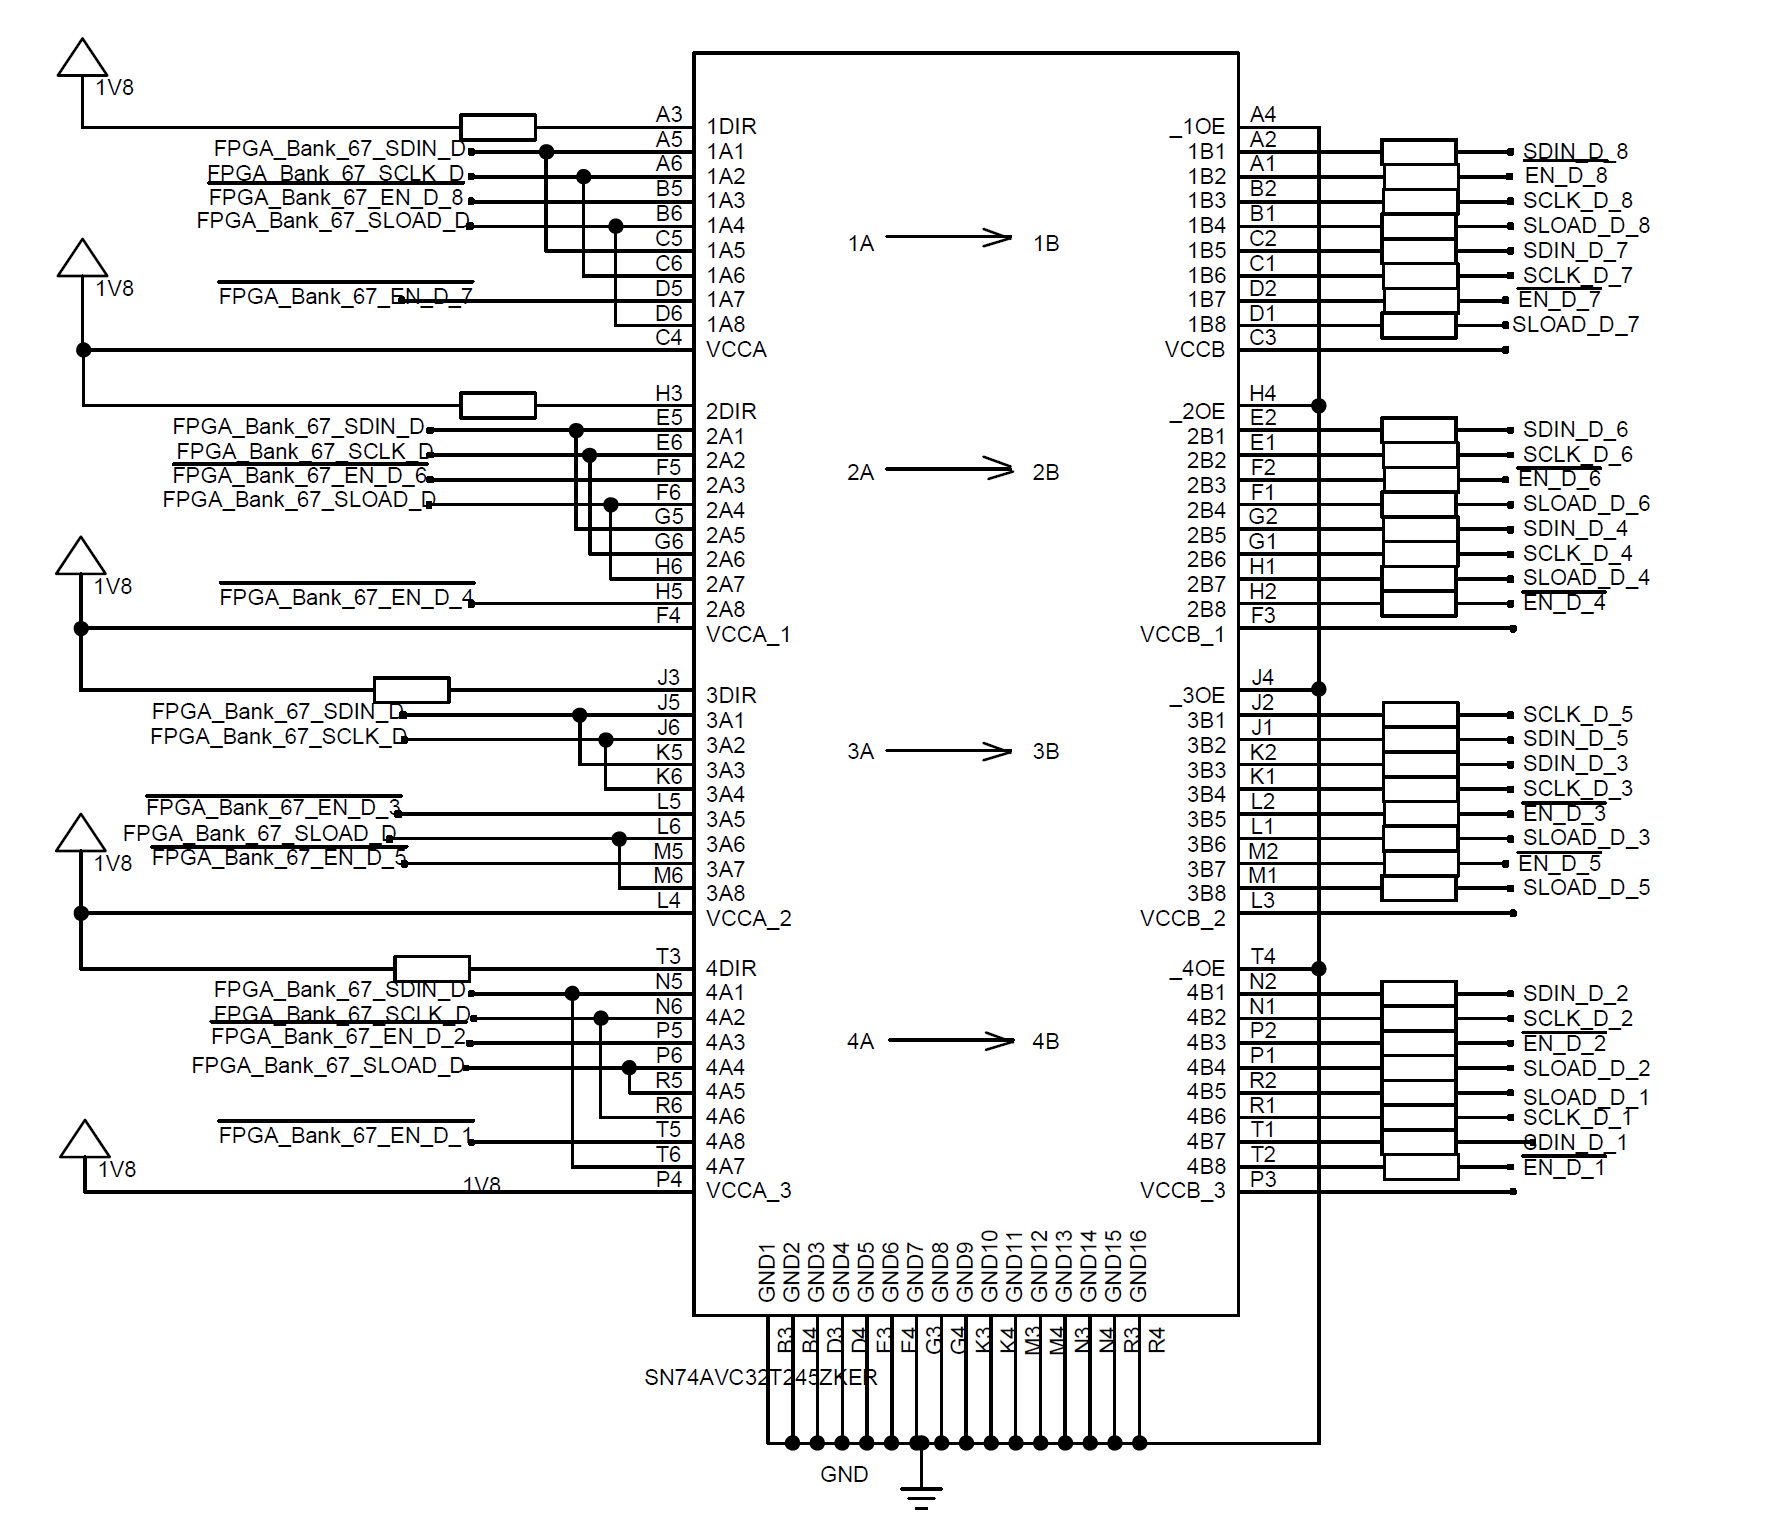
\includegraphics[width = \textwidth]{chap/04-theresa/img/schematic/level_trans}
	\caption[SN74AVC32T245 bus transceiver]{Schematic of the SN74AVC32T245 bus transceiver}
	\label{fig:level_trans}
\end{figure}

\paragraph{Outputs}
The output of the delay chip is using a \gls{lvpecl} signaling interface, which is based on an open-emitter topology (see \autoref{fig:lvpecl}).
This requires a path to \gls{dc}, which is achieved by adding \SI{140}{\ohm} resistors (recommended in the data sheet).

\begin{figure}[H]
	\centering
	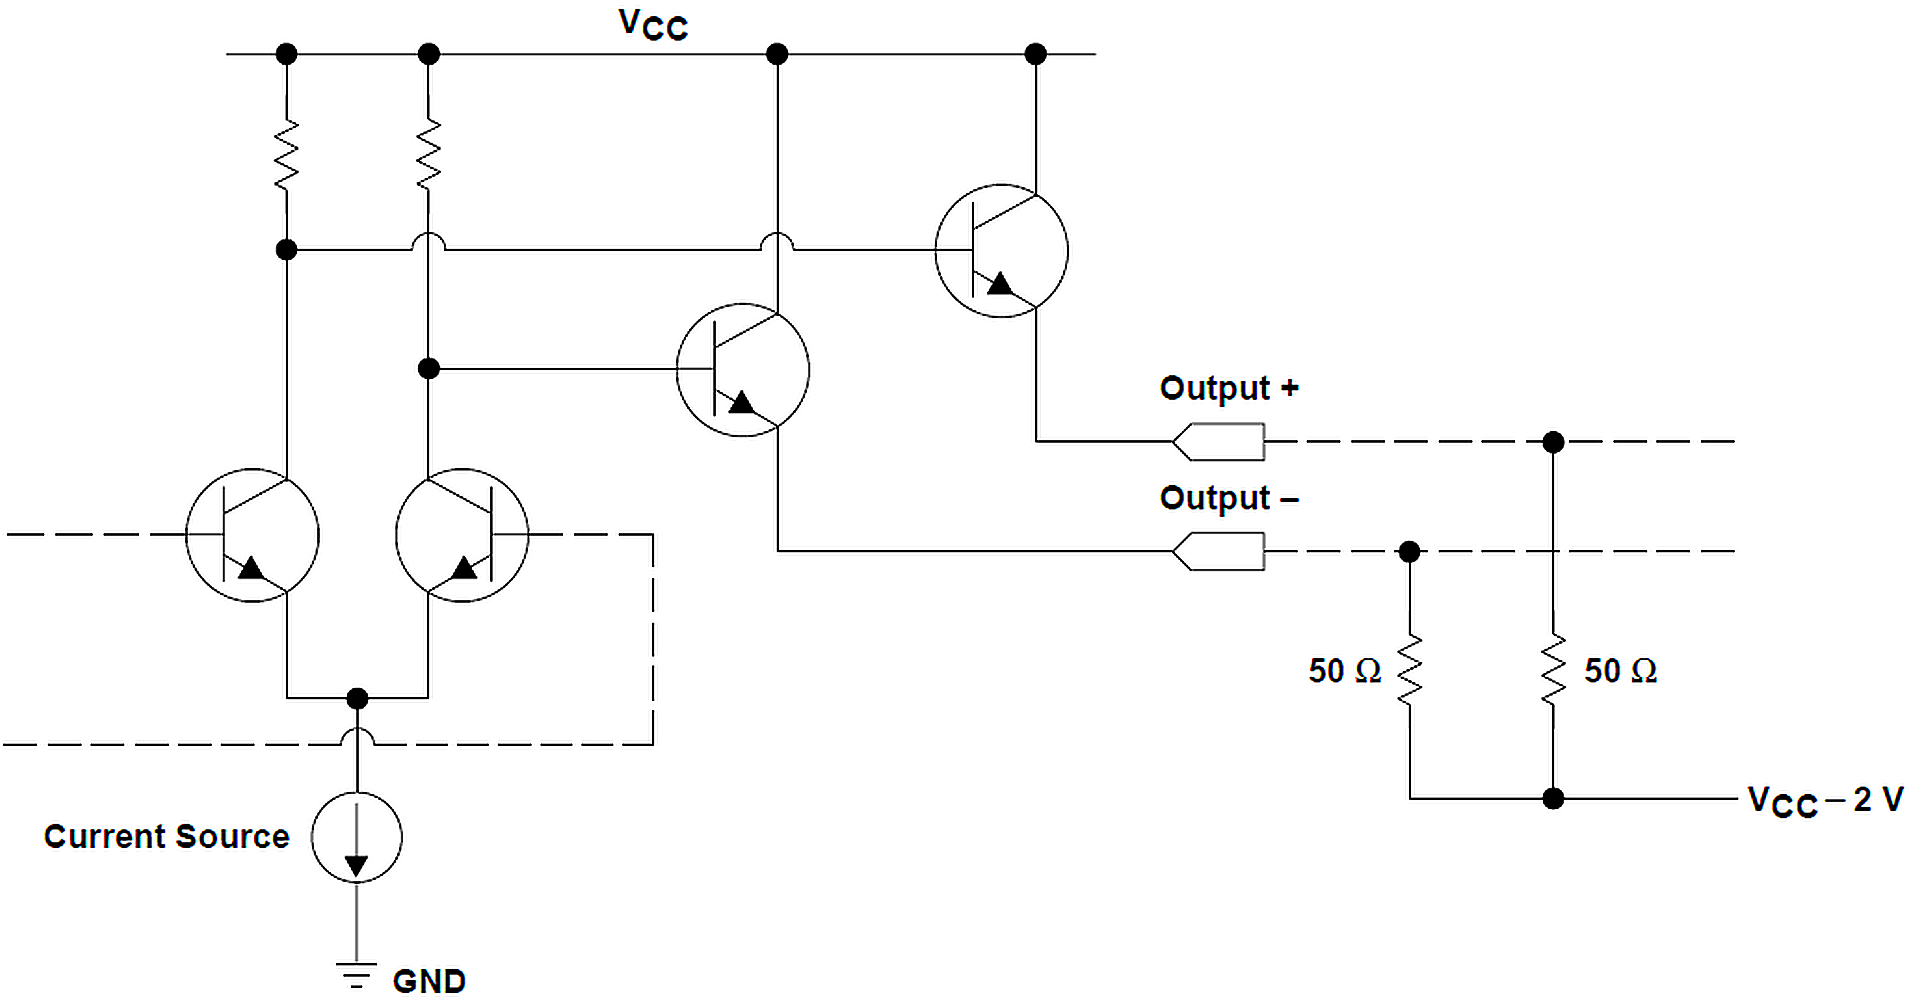
\includegraphics[width = \textwidth]{chap/04-theresa/img/lvpecl}
	\caption[LVPECL driver topology]{LVPECL driver topology. Left side shows the emitter-follower based driver. On the right, an example biasing with resistors is shown. \cite{lvpecl}}
	\label{fig:lvpecl}
\end{figure}
%TODO to tikz

As the output will be connected to the \gls{tha}, it is necessary to check the compatibility of the maximum amplitude and common-mode of the pins.

According to the data sheet \cite{NB6L295}, the voltage level of the output can vary between  $V_\text{cc} - \SI{1825}{\milli\volt}$ and $V_\text{cc} - \SI{825}{\milli\volt}$ (see \autoref{tab:nb6l295}).
Maximal voltage amplitude acceptable by the \gls{tha} inputs is \SI{2000}{\milli\volt} (see \autoref{tab:hmc5640}).
When using a supply voltage of $V_\text{cc} = \SI{3.3}{\volt}$, provided e.g. by the read-out card through the \gls{fmc}+ connector, this leads to a maximum output level of \SI{2475}{\milli\volt}.
This exceeds the limit given by the \gls{tha}.
Therefore, for $V_\text{cc}$ a smaller voltage should be considered.
In this design a voltage of $V_\text{cc} = \SI{2.5}{\volt}$ is chosen, which guarantees that the amplitude falls within the range \SIrange{675}{1675}{\milli\volt}.

The second point to consider is the common mode voltages. 
According to the data sheet of the \gls{tha}, the common mode voltage of the input clock pins is \SI{0.1}{\volt} (see \autoref{tab:hmc5640}).
The common mode voltage of the delay chip is not explicitly mentioned in the data sheet, thus it has to be calculated.

\clearpage
The common mode voltage $V_\text{CM}$ is just the mean value between the HIGH level and the LOW level voltage of the output pins:
\begin{equation}
	V_\text{CM} = \frac{V_\text{out, LOW} + V_\text{out, HIGH}}{2}.
\end{equation}
According to this, the common mode voltage $V_{\text{CM}}$ of the delay chip output, when taking the minimum/maximum voltage level values, is 
\begin{equation}
	V_\text{CM} = \frac{\SI{675}{\milli \volt} + \SI{1675}{\milli \volt}}{2} = \SI{1175}{\milli \volt}.
\end{equation}
This is higher than the maximal input common mode voltage of the \gls{tha}.
\gls{ac} coupling is therefore necessary in this case, i.e. connecting the pins via capacitors.

\subsection{Clock Distribution}
The clock distribution is designed as shown in \autoref{fig:clocking}.
%todo anchor south west
\begin{figure}[tb]
	\centering
	\includegraphics[width = \textwidth]{chap/04-theresa/img/pll/clocking_arch}
	\caption{Overview of the clocking paths on the sampling board}
	\label{fig:clocking}
\end{figure}
The LMK04808B low-noise clock jitter cleaner with dual-loop \glspl{pll} from \textit{Texas Instruments} cleans the incoming reference clock provided from the system (e.g. from \gls{kara}) for high temporal precision \cite{caselle2013}.
It is used with an external \gls{vcxo} from \textit{ABRACON}. 

The LMK04808B contains two \glspl{pll} (therefore called ``dual-loop''). 
The first \gls{pll} is used to clean the reference clock from jitter. 
The second is then used to generate and distribute the cleaned clock signals to the outputs of the components.

The time skew between the \gls{pll} outputs lies in the range of \SI{30}{\pico \second} (see \cite{lmk04808b}).
This is higher than the \SI{11}{\pico \second} delay step of the delay chips, not allowing for precise time delay control. 
In order to guarantee low time skew (range of few picoseconds), two fanout buffers are used to distribute the cleaned clock signal to the components on the board.
The fanout buffers used are the HMC987LP5E from \textit{Analog Devices}.
The time skew of these components between channels typically lies in the range of \SI{1.5}{\pico \second}, 20 times smaller than the time skew of the \gls{pll}.
As one fanout buffer has eight outputs, two chips are needed to cover all 16 sampling channels. 
Each fanout receives the clock reference from one output of the LMK0480B. 
To ensure exactly identical clocking signals between the two fanouts they are connected to two outputs of the same output group of the LMK0480B.

The maximum output frequency of the LMK04808B is \SI{1536}{\mega \hertz}, which is not enough to clock the \glspl{adc} at maximum sampling rate (\SI{2.5}{\giga \sample \per \second}). 
A second kind of \gls{pll} is therefore needed to provide programmable reference clocks to the \glspl{adc} and \glspl{dac}.
As \autoref{fig:clocking} shows, the LMK04808B also provides a clocking signal to other \glspl{pll}, the LMX2594 from \textit{Texas Instruments}.
This \gls{pll} is able of clocking signal frequencies up to \SI{15}{\giga \hertz}.

Due to the \gls{adc} clocking limitations on the read-out card explained in \autoref{ssec:interl_impl}, two of the \glspl{pll} are needed. 
The reference clock signal is provided by outputs from different output groups of the LMK04808B. This way, the phase of each reference clock can be programmed individually, which allows to implement the \gls{adc} clocking technique described in \autoref{ssec:interl_impl}.

One output of the \gls{pll} is propagated to the \gls{fmc}+ connector as reference clock for the \gls{fpga}.


\subsubsection*{PLLs}
A \gls{pll} is a control loop, used to synchronize an output oscillator signal with a reference signal.
The principle lies in comparing the phases between the two inputs. 
When there is a varying phase difference, it means that the signals are at different frequencies.
As soon as the phase difference stays constant, it means that both of the frequencies are the same or one is a multiple of the other. 
In this state the \gls{pll} is called to be ``locked''.
The general architecture of a \gls{pll} is shown in \autoref{fig:pll_block}.
\begin{figure}[H]
	\centering
	\includegraphics[width = \textwidth]{chap/04-theresa/img/pll/pllBlock.tikz}
	\caption[PLL block diagram]{General block diagram of a \gls{pll} \cite{pll_design}}
	\label{fig:pll_block}
\end{figure}
For proper noise performance, a properly designed loop filter for both \glspl{pll} is needed. 
The output of the loop filter is the voltage for controlling the \gls{vco}.
The \gls{vco} output of is a frequency $f_\text{VCO}$ proportional to the applied voltage.
$f_\text{VCO}$ is divided by the \textit{N Divider} to the frequency $f_n$ and then compared to the phase detector frequency $f_\text{PD}$ in the phase detector. 
$f_\text{PD}$ results from dividing the reference frequency $f_\text{OSC}$ with an \textit{R divider}. 
The phase detector produces current correction pulses (with magnitude $K_\text{PD}$) with a duty cycle proportional to the phase error between $f_\text{PD}$ and $f_n$. 
These pulses are filtered by the low pass loop filter, which basically converts these pulses into a voltage. \cite{pll_design}
The loop filter is one of the key component determining the \gls{pll} performance (concerning jitter, noise, \ldots) and therefore has to be designed carefully.


To calculate the loop filter, the \textit{Texas Instruments} \textit{PLLatinum Sim} tool is used. 
This tool provides a convenient way to calculate the necessary loop filter components, given the \gls{vco} characteristics, desired filter order, charge pump current and desired performance (e.g. optimize jitter). 
A passive fourth order loop filter is shown in \autoref{fig:loop_filter}.
In order to implement a lower order filter, some components need to be left out.
To implement an active filter an additional operational amplifier is necessary.
The input of the filter is connected to the output of the charge pump from which it receives the current pulses.
The output of the filter is the voltage $V_\text{tune}$ which is the input to the \gls{vco}.
\begin{figure}[tb]
	\centering
	\tikzexternaldisable
	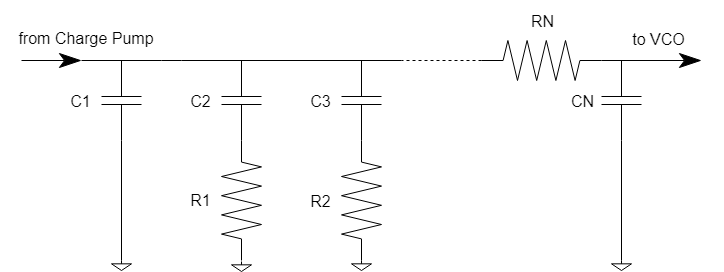
\includegraphics[width = \textwidth]{chap/04-theresa/img/pll/loop_filter.tikz}
	\caption[PLL loop filter components]{Passive fourth order loop filter for PLL}
	\tikzexternalenable
	\label{fig:loop_filter}
\end{figure}
The LMK04808B has two \glspl{pll} inside (PLL1 and PLL2).
For both, the loop filter has to be calculated separately. 
Both filters are implemented as second order filters, the calculated parameters are listed in \autoref{tab:lmk04808B_filter}.
Note that PLL2 has already a partially integrated loop filter.
\begin{table}[H]
	\caption[LMK04808B loop filter characteristics]{Loop filter characteristics of the LMK04808B}
	\label{tab:lmk04808B_filter}
	\centering
	\begin{tabularx}{\textwidth}{Xl}
		\toprule
		\textbf{Parameter}                                                        & \textbf{Value}           \\ \midrule
		                            \multicolumn{2}{c}{\textbf{PLL1 parameters}}                             \\
		VCO Gain                                                                  & \SI{0.15}{\MHz\per\volt} \\
		Loop Bandwidth                                                            & \SI{0.2578}{\kHz}        \\
		Phase Margin                                                              & \ang{70}                 \\
		Effective Charge Pump Gain                                                & \SI{0.4}{\milli\ampere}  \\
		Phase Detector Frequency                                                  & \SI{25}{\MHz}            \\
		VCO Frequency                                                             & \SI{200}{\MHz}           \\
		                    \multicolumn{2}{c}{\textbf{Loop filter components for PLL1}}                     \\
		$C_{1}$                                                                   & \SI{39}{\nano\farad}     \\
		$C_{2}$                                                                   & \SI{1800}{\nano\farad}   \\
		$R_{2}$                                                                   & \SI{2.2}{\kilo\ohm}      \\
		[0.3cm]
	    \multicolumn{2}{c}{\textbf{PLL2 parameters}}                   \\
		VCO Gain                                                                  & \SI{30}{\MHz\per\volt}   \\
		Loop Bandwidth                                                            & \SI{390.9624}{\kHz}      \\
		Phase Margin                                                              & \ang{70}                 \\
		Effective Charge Pump Gain                                                & \SI{1.6}{\milli\ampere}  \\
		Phase Detector Frequency                                                  & \SI{50}{\MHz}            \\
		VCO Frequency                                                             & \SI{3000}{\MHz}          \\
		[0.3cm]
	    \multicolumn{2}{c}{\textbf{Loop filter components for PLL2}}   \\
		$C_{1}$                                                                   & \SI{22}{\pico\farad}     \\
		$C_{2}$                                                                   & \SI{2.2}{\nano\farad}    \\
		$R_{2}$                                                                   & \SI{3.3}{\kilo\ohm}      \\ \bottomrule
	\end{tabularx}
\end{table}

The loop filter for the LMX2594 is designed in the same way as described above with the \textit{PLLatinum Sim} tool. 
The calculated values for the components to be implemented are shown in \autoref{tab:lmx2594_filter}.
The filter is implemented as a third order passive filter.
The schematic and layout of the filter have been implemented in a way to enable alteration of the filter, i.e. changing the filter order or component values.
The schematic and layout have been implemented in order to enable flexible change.
This gives the possibility to experimentally find the correct order and components for best performance by real measurements with the board.
The schematic of the LMX2594 is shown in \autoref{fig:lmx2594}.

\begin{figure}[H]
	\centering
	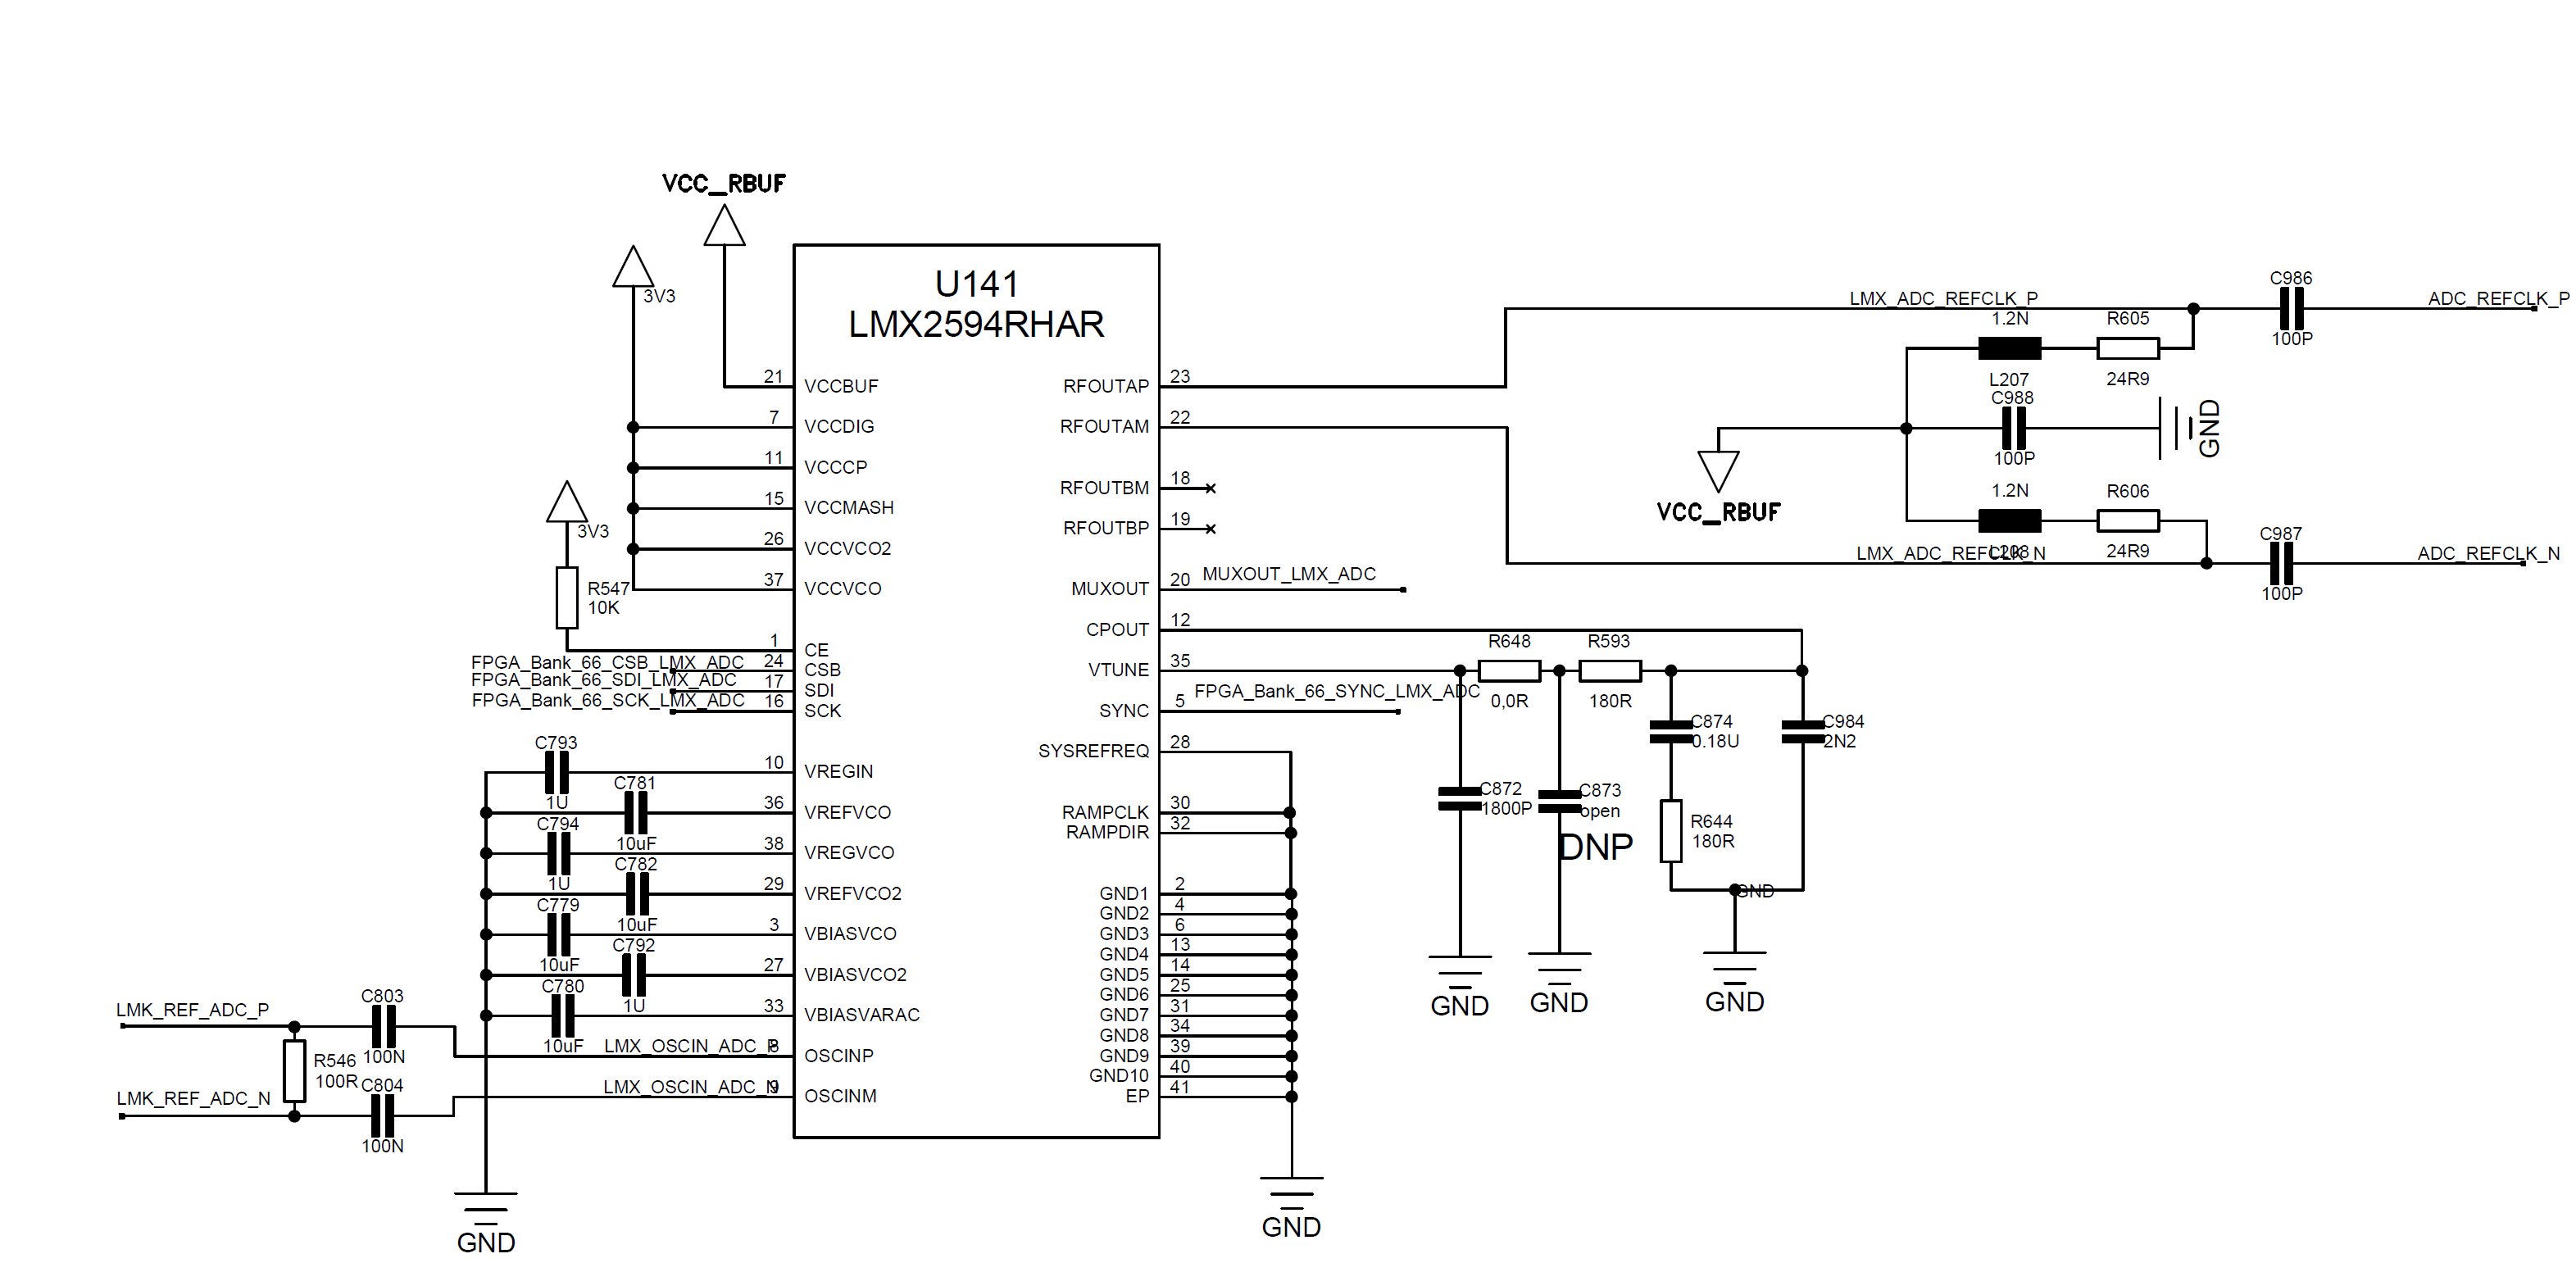
\includegraphics[width = \textwidth]{chap/04-theresa/img/schematic/lmx2594}
	\caption{Schematics of the LMX2594}
	\label{fig:lmx2594}
\end{figure}

\begin{table}[tb]
	\caption[LMX2594 loop filter characteristics]{Loop filter characteristics of the LMX3594}
	\label{tab:lmx2594_filter}
	\centering
	\begin{tabularx}{\textwidth}{Xl}
		\toprule
		\textbf{Parameter}                         & \textbf{Value}             \\ 
		\midrule
		\multicolumn{2}{c}{\textbf{PLL parameters}}                             \\
		VCO Gain                                   & \SI{239}{\MHz\per\volt}    \\
		Loop Bandwidth                             & \SI{32.7}{\kHz}            \\
		Phase Margin                               & \ang{69}                   \\
		Effective Charge Pump Gain                 & \SI{3}{\milli\ampere}      \\
		Phase Detector Frequency                   & \SI{24.576}{\MHz}          \\
		VCXO Frequency                             & Designed for \SI{15}{\GHz} \\
		[0.3cm]
		\multicolumn{2}{c}{\textbf{Loop filter components}}   \\                        
		$C_{1}$                          & \SI{2200}{\pico\farad}     \\
		$C_{2}$                          & \SI{180}{\nano\farad}      \\
		$C_{3}$                          & \SI{1800}{\pico\farad}     \\
		$R_{2}$                                    & \SI{160}{\ohm}             \\
		$R_{3}$                          & \SI{180}{\ohm}             \\ \bottomrule
	\end{tabularx}
\end{table}



\subsubsection*{Fanout Buffer}
The fanout buffer receives as input the clock signal from the main \gls{pll} and distributes it to the delay chips.
In this design, the HMC987LP5E from \textit{Analog Devices} is chosen due to its low jitter and low skew performance. 
The schematics of the chip is shown in \autoref{fig:fanout}.
\begin{figure}[H]
	\centering
	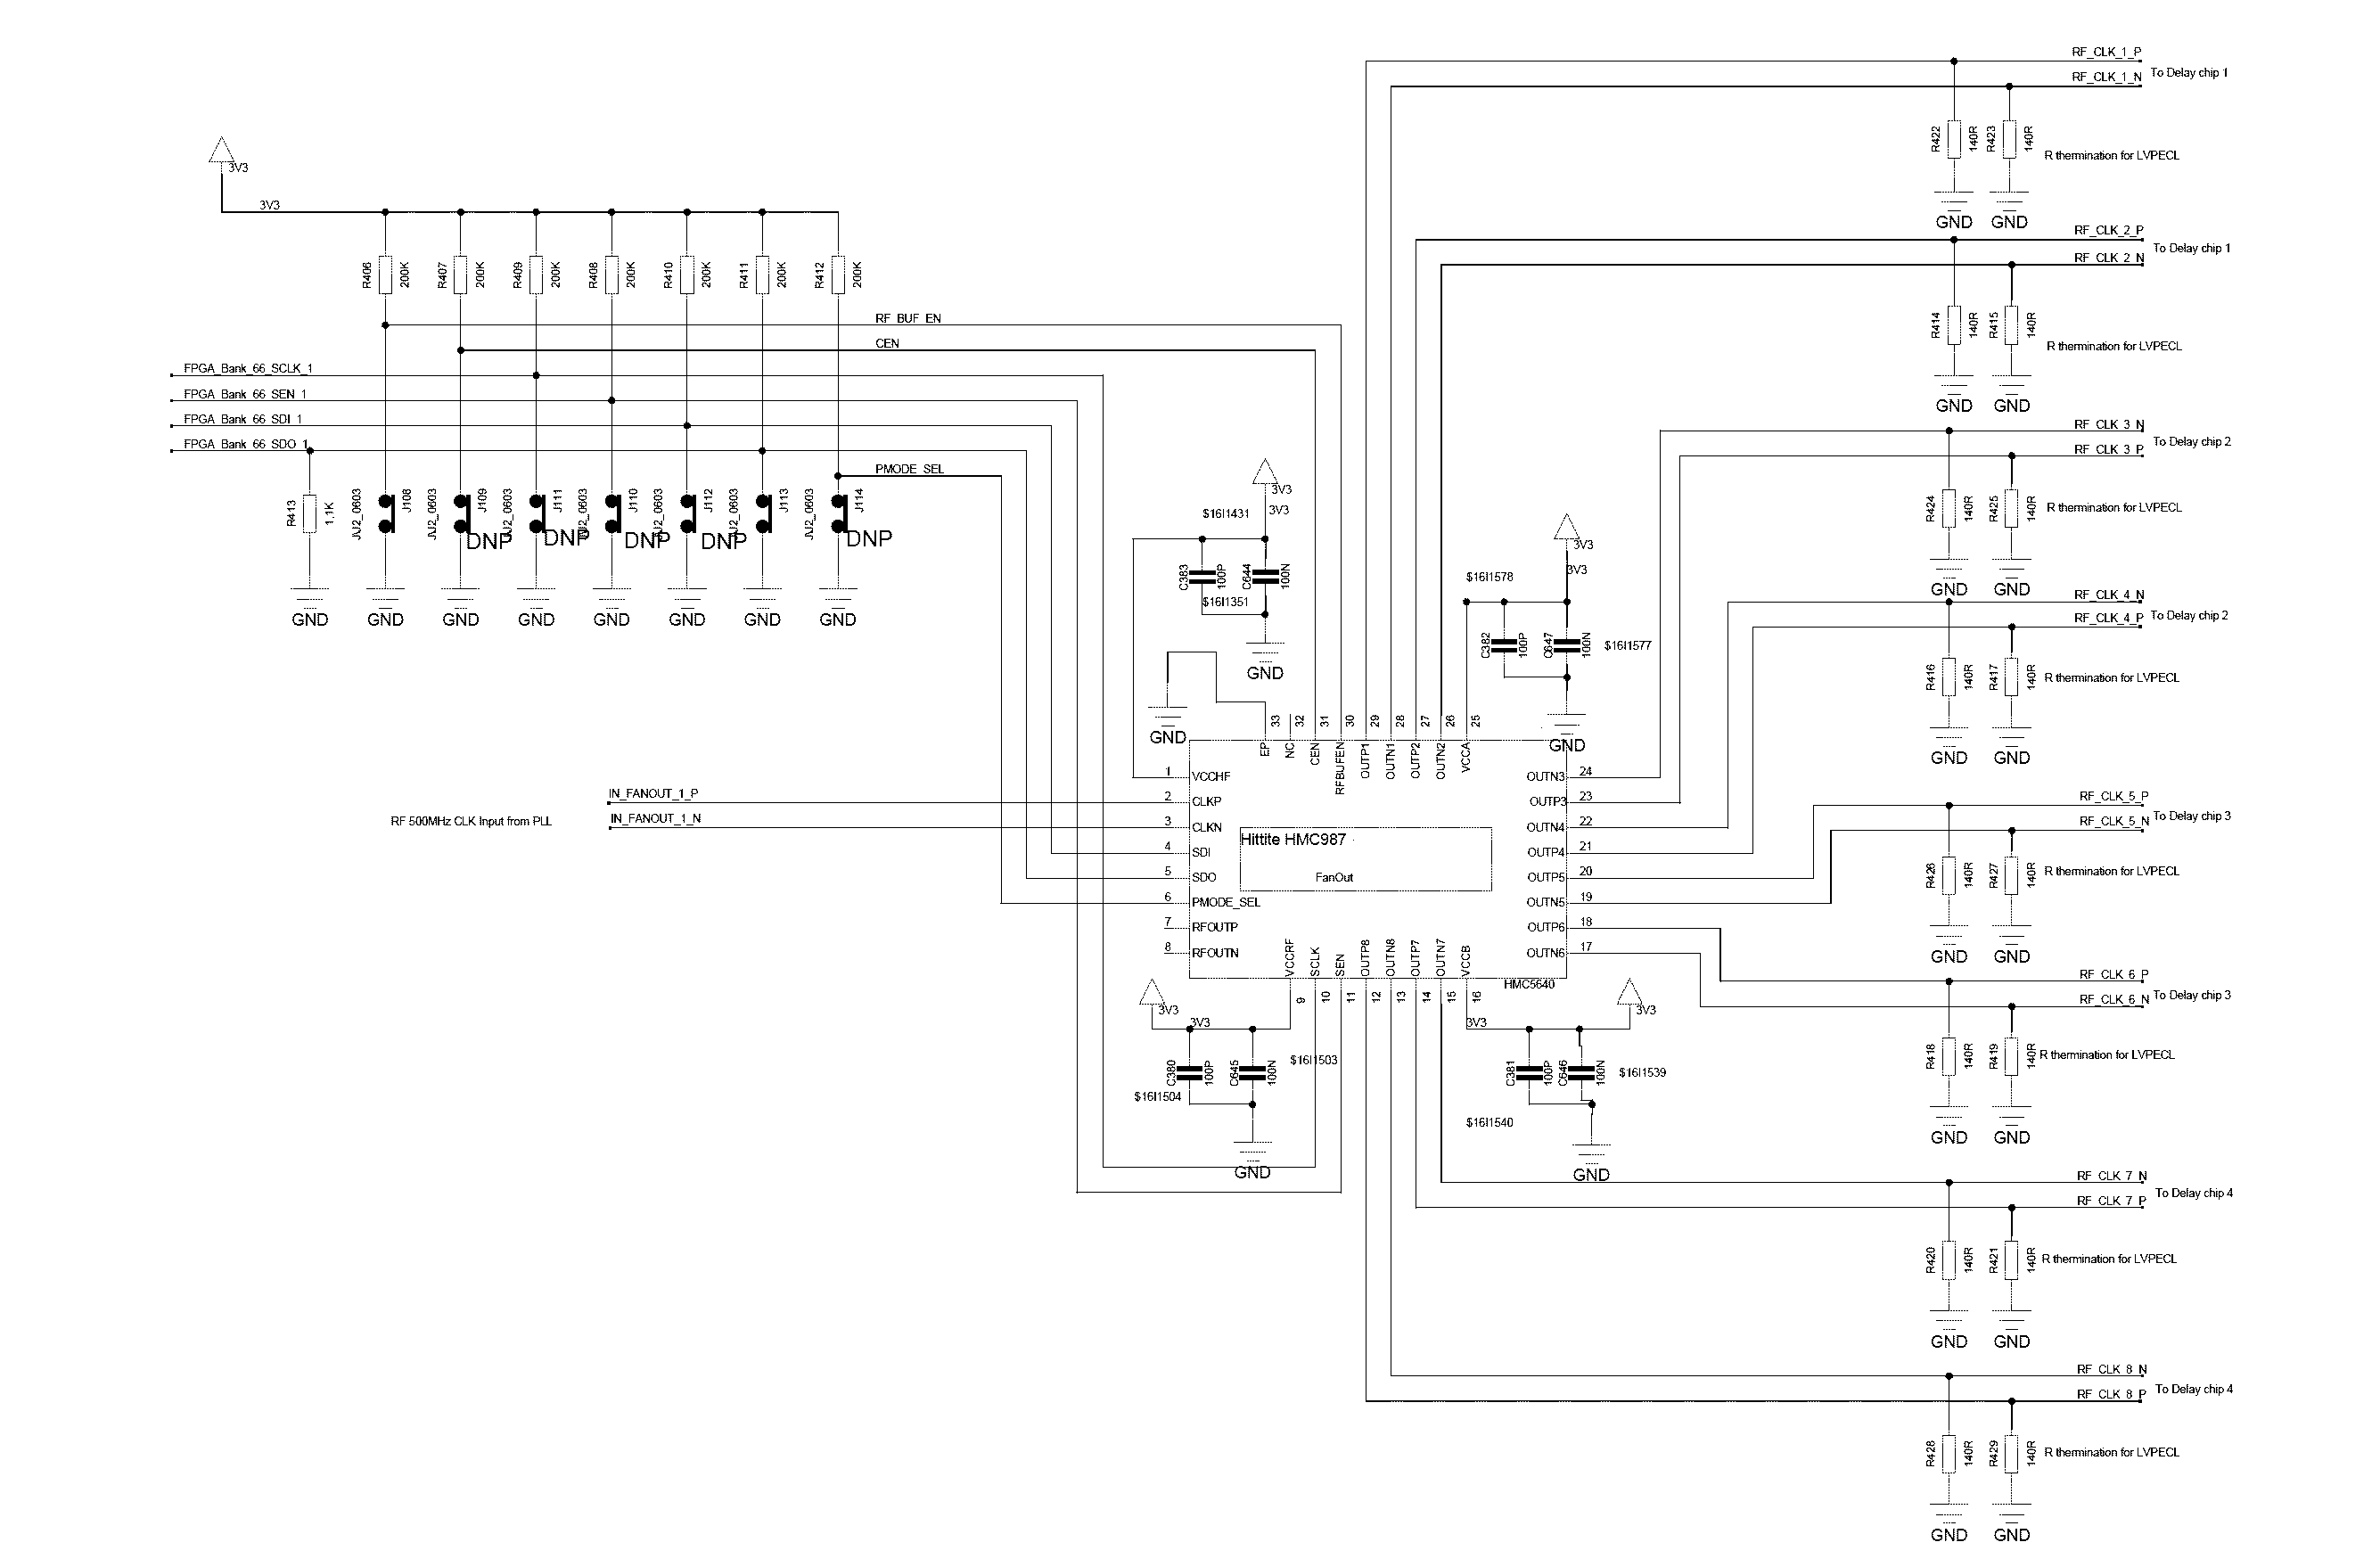
\includegraphics[width = 0.9\textwidth]{chap/04-theresa/img/schematic/fanout}
	\caption{Schematic of the fanout}
	\label{fig:fanout}
\end{figure}
Decoupling capacitors are placed at every power supply pin in order to guarantee a clean and stable voltage level.

The outputs of the fanout buffer are based on \gls{lvpecl} signaling interfaces and therefore need to be connected to ground via resistors.
Individual outputs can be enabled or disabled either via \gls{spi} (setting pin \texttt{PMODE\_SEL} to '0') or by using parallel pin control (setting pin \texttt{PMODE\_SEL} to '1'). 

In parallel pin control the \gls{spi} pins \texttt{SCLK}, \texttt{SDI} and \texttt{SEN} are reinterpreted as a 3-bit control bus.
In this mode, the pins are either pulled up to $V_\text{cc}$ or connected to ground via on-board jumpers to represent a logic '1' or '0'.
For the design, the parallel pin control mode is selected, therefore the \texttt{PMODE\_SEL} pin is pulled up to $V_\text{cc}$ ($\eqdev$ logic '1').
In order to have the opportunity to enable the \gls{spi} mode in later usage, a jumper is placed at this pin so that it can be connected to ground if necessary ($\eqdev$ logic '0', enabling \gls{spi} mode).
The \texttt{SCLK}, \texttt{SDI} and \texttt{SEN} pins are connected to the \gls{fmc}+ connector.
To enable all outputs, the \gls{spi} pins need to be set to '111' according to the data sheet, i.e. pulled-up to $V_\text{cc}$. 
Here, jumpers are foreseen as well, to allow enabling/disabling in later usage.

\subsection{Digital-To-Analog-Converter Channels}
For test purposes, two \gls{dac} channels from the read-out card are routed on the sampling board.
In this way, a programmable analog waveform can be generated by \gls{fpga}, without the need for an external signal generator. 
The differential inputs from the \glspl{dac} are transformed into single ended outputs with dedicated baluns\footnote{\textbf{bal}anced to \textbf{un}balanced}. the BD3150N50100AHFa and the BD4859N50100AHF from \textit{Anaren}. 
These are used for the signal frequency range \SIrange{3.1}{5.0}{\GHz} and \SIrange{4.8}{5.9}{\GHz} respectively.
The single-ended output is connected to a miniature \gls{rf} connector from \textit{Hirose Electric}.

The programmable analog waveform, generated by the \gls{dac} (operating up to \SI{10}{\giga \sample \per \second}), can be applied to the input of the sampling board as a test signal and be employed for testing, characterizing and calibrating each sampling channel individually.

The schematic of a \gls{dac} channel is shown in \autoref{fig:dac_channel}.
\begin{figure}[H]
	\centering
	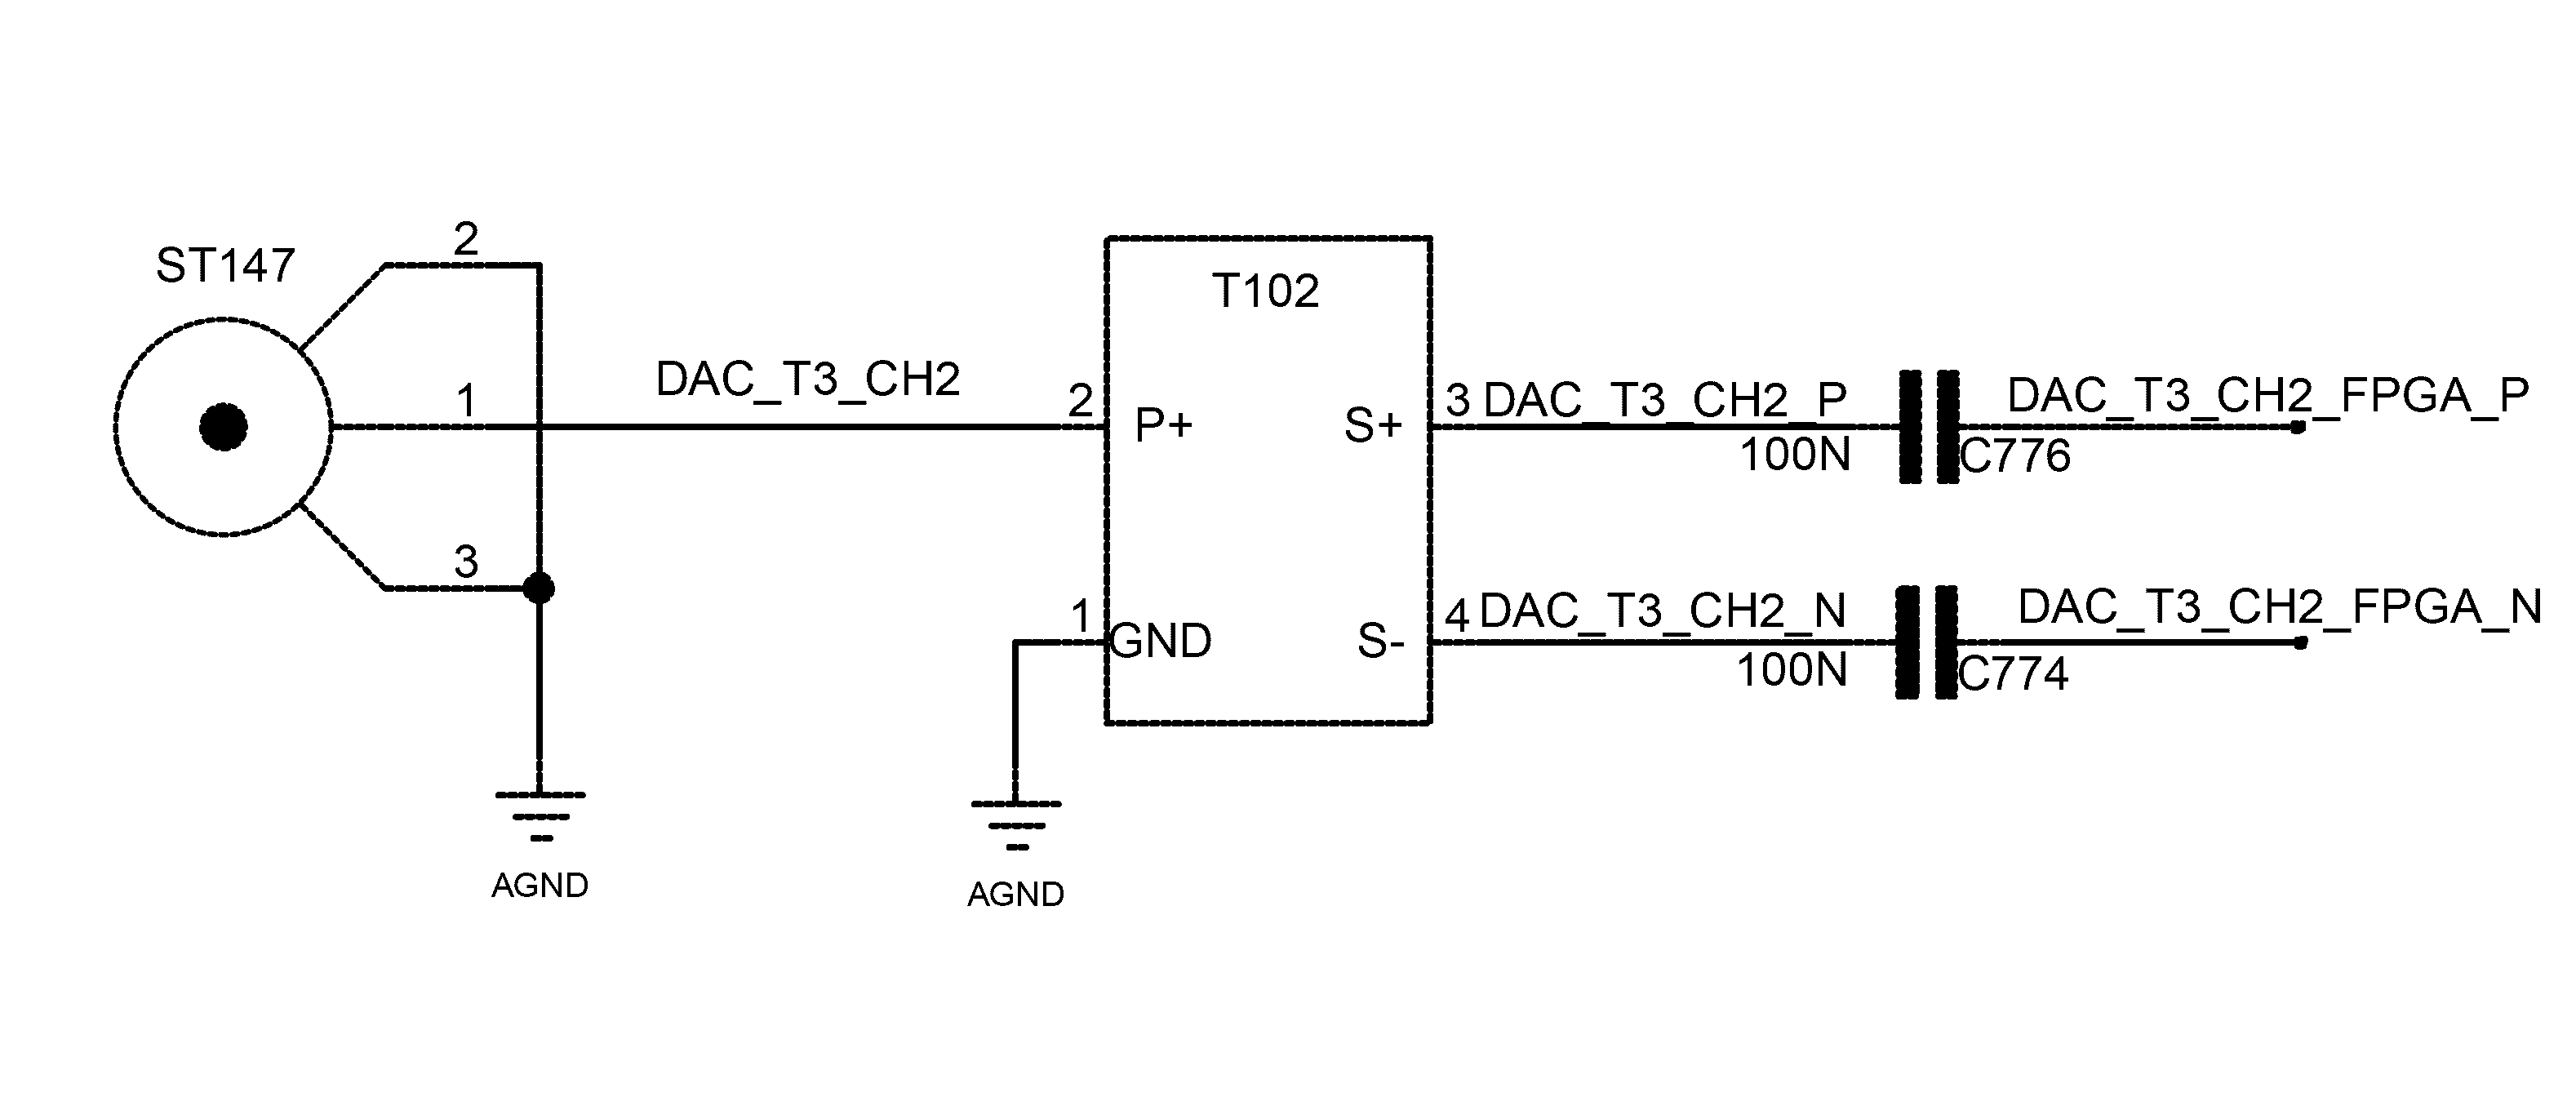
\includegraphics[width = 0.8\textwidth]{chap/04-theresa/img/schematic/dac_channel}
	\caption{DAC-channel with balun. Signal propagates from right to left.}
	\label{fig:dac_channel}
\end{figure}


\subsection{Power Supply}
Low-ripple power supply is an important point key for low noise performance of the board. Especially high-performance \Glspl{ic}, such as \glspl{tha}, highly rely on a low-ripple voltage level for correct functionality. 
Therefore, proper power supply design is an important step which needs to be handled with care.
This step includes the selection the right type voltage regulators, as well as providing appropriate filtering. 
Furthermore, in order 

\autoref{tab:theresacomp} lists the power supply requirements of all the components used on the board.

\begin{table}[H]
	\caption{Power consumption of components on the board}
	\label{tab:theresacomp}
	\begin{minipage}{\textwidth}
		\centering
		\begin{tabularx}{\textwidth}{Xlllll}
			\toprule
			\textbf{Component}         & $V_\text{cc}$ (V) & $I_\text{max}$ (A)                        & $P_\text{max}$ (W) & $\#_\text{parts}$ & $I_\text{tot, max}$\footnote{for 16 \glspl{adc}} (A) \\ \midrule
			HMC5649 (\gls{tha})        & 2                 & 0.221                                     & 0.442              & 16                & 3.536                                                \\
			NB6L295 (Delay chip)       & 2.5               & 0.170                                     & 0.425              & 8                 & 1.36                                                 \\
			HMC987LP5E (Fanout) & 3.3               & 0.234\footnote{All Outputs and RF-Buffer} & 0.772              & 2                 & 0.468                                                \\
			LMK04808B (\gls{pll})      & 3.3               & 0.590\footnote{All CLKs}                  & 1.947              & 1                 & 0.590                                                \\
			LMX2594 (\gls{pll})        & 3.3               & 0.340                                     & 1.122              & 2                 & 2.244                                                \\
			VCXO                       & 3.3               & 0.03                                      & 0.198              & 1                 & 0.03                                                 \\ \bottomrule
		\end{tabularx}
	\end{minipage}
\end{table}
In general, there are four different voltage supplies provided by different sources:
\begin{itemize}
	\item \SI{1.8}{\volt} for digital components coming from \gls{fmc}+ connector
	\item \SI{3.3}{\volt} for digital components coming from \gls{fmc}+ connector
	\item \SI{3.3}{\volt} and \SI{-5}{\volt} for analog devices from external power supplies 
\end{itemize}
An \gls{emi} filter needs to be placed in order to reduce the electromagnetic interference from external sources. 
The filter used is a passive LC low pass filter, the schematic fo which is shown in \autoref{fig:emi_filter}.
It consists of a inductor and several shunting capacitors.
This configuration guarantees that high frequency components on the power supply voltage are reduced and high frequency currents are redirected to ground through the capacitors.
At each power supply one \gls{emi} filter has been placed. 
\begin{figure}[tb]
	\centering
	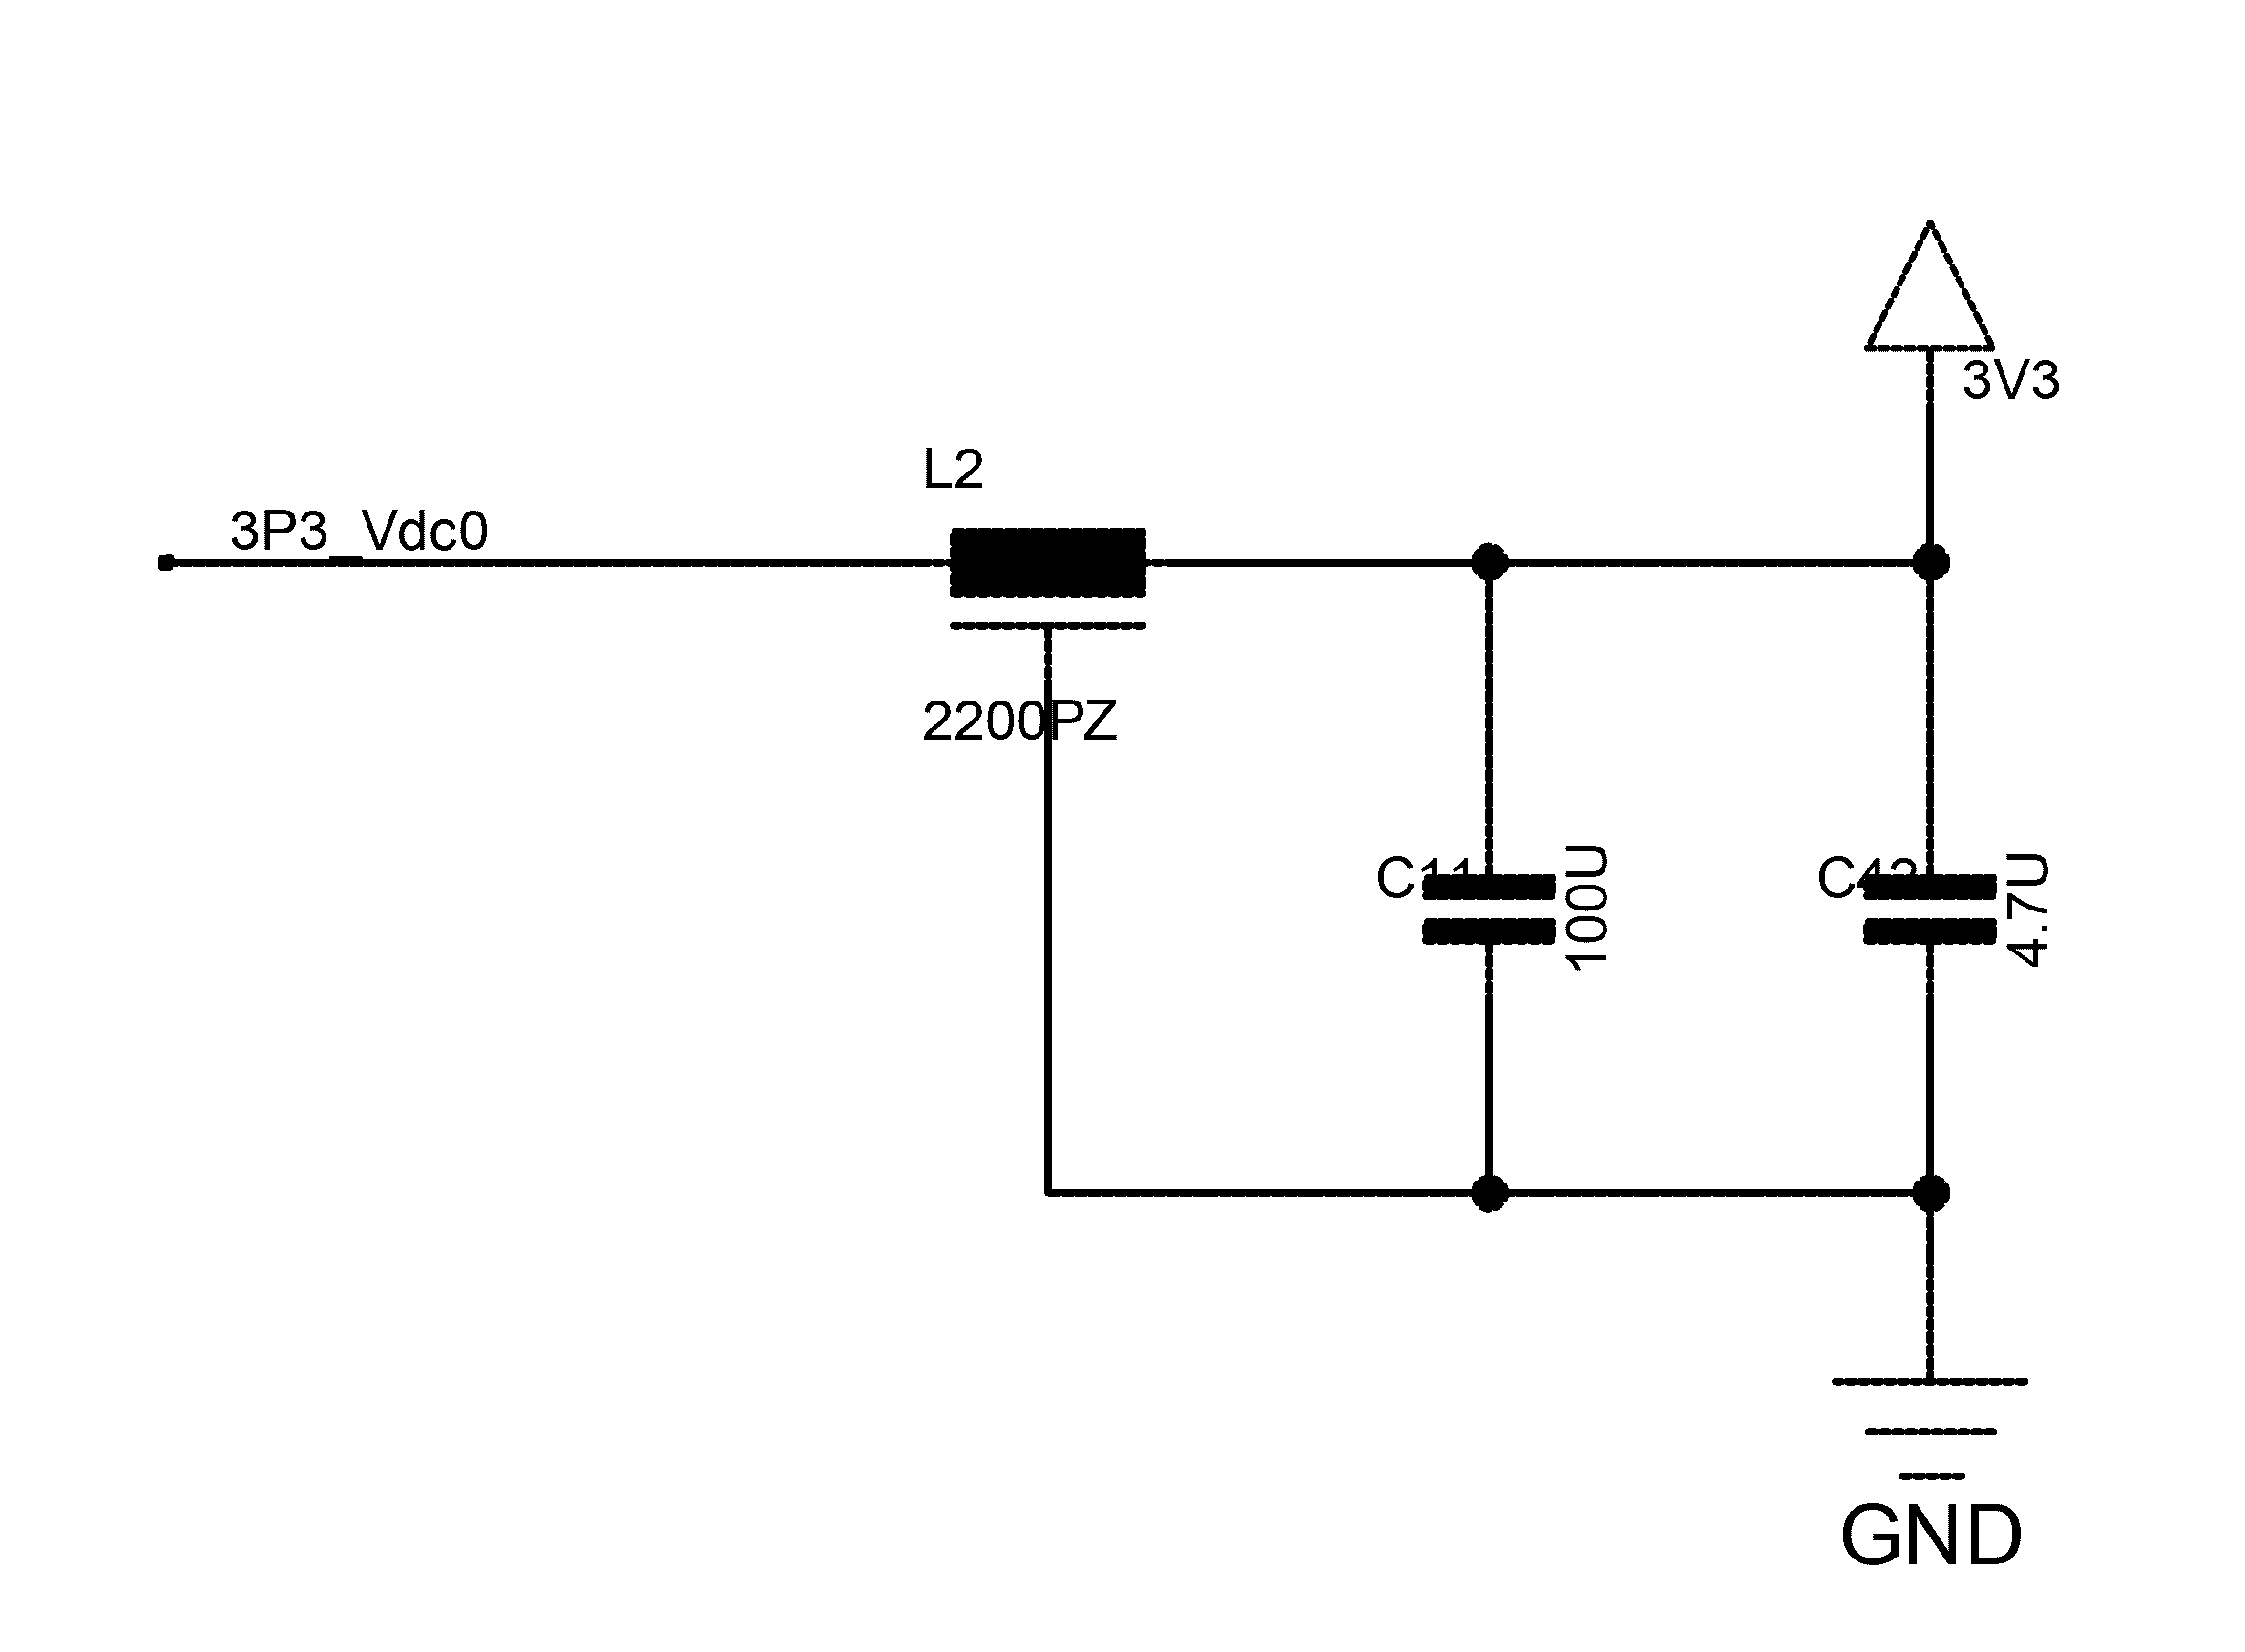
\includegraphics[width = 0.7\textwidth]{chap/04-theresa/img/schematic/emi_filter.tikz}
	\caption{EMI-filter used for filtering power supply}
	\label{fig:emi_filter}
\end{figure}
For the sensitive components like \gls{tha} voltage regulators have to be used to guarantee low noise operation.


\subsubsection*{Voltage Regulator for Track-and-Hold-Amplifiers}
The \glspl{tha} need a low-ripple voltage level for optimal operation. 
Linear voltage regulators are capable to maintain a stable output voltage and are therefore to be used with the \glspl{tha}.

On the \gls{kapture} sampling board, the \gls{ldo} ADP1708 from \textit{Analog Devices} is used to provide a power supply for the \glspl{tha}. 
A \gls{ldo} is able to operate at a low potential difference between the input and output voltage. 
This low potential difference has the benefit of low power dissipation, which also reduces the heat produced by the components.  
This power supply can provide a maximum of \SI{1}{\ampere} to the load. 
In order to minimize the amount of components needed on the board and to save space, a different \gls{ldo} which provides higher currents should be used. 
This way, one single voltage regulator can be used for more components.

For the new board, the ADP1741 low-dropout voltage regulator from \textit{Analog Devices} has been selected. This voltage regulator has adjustable output voltage from \SIrange{1.6}{3.6}{\volt} and a maximum output current of \SI{2}{\ampere}. 

It is necessary to think about the number of voltage regulators needed. As a rule of thumb, the power supply should provide at least twice the maximum current (i.e. power) needed by the components it drives. \cite{michele} The power consumption/maximum current for the \glspl{tha} are listed in \autoref{tab:theresacomp}. 

The maximal output current $I_\text{max, LDO}$ from the ADP1741 is \SI{2}{\ampere}.
With the rule mentioned above and the maximal current draw $I_\text{m, THA}$ = \SI{0.221}{\ampere} from the \gls{tha}, the maximal number of components $N$ which the \gls{ldo} can handle is calculated as 

\begin{align*}
	I_\text{max, LDO}                              & > 2 \cdot N \cdot I_\text{m, THA} \\
	I_\text{max, LDO}/(2 \cdot I_\text{m, THA})    & > N                               \\
	\SI{2}{\ampere} / (2\cdot \SI{0.221}{\ampere}) & > N                               \\
	4.52                                           & > N \quad \rightarrow N = 4
\end{align*}
This means, 4 \glspl{ldo} are needed to cover 16 \glspl{tha}.

The output voltage level of the regulator is set by an external divider with the resistors $R_1$ and $R_2$ (refer to \autoref{fig:adp1741}). According to the data sheet \cite{adp1741}, the voltage $V_\text{OUT}$ is determined by
\begin{equation}\label{eq:ldo}
	V_\text{OUT} = \SI{0.5}{\volt}\left(1 + \frac{R_1}{R_2} \right).
\end{equation}
In order to achieve the required \SI{2}{\volt}, the values of the resistors are chosen to $R_1 = \SI{30}{\kilo\ohm}$ and $R_2 = \SI{10}{\kilo \ohm}$. 

\begin{figure}[tb]
	\centering
	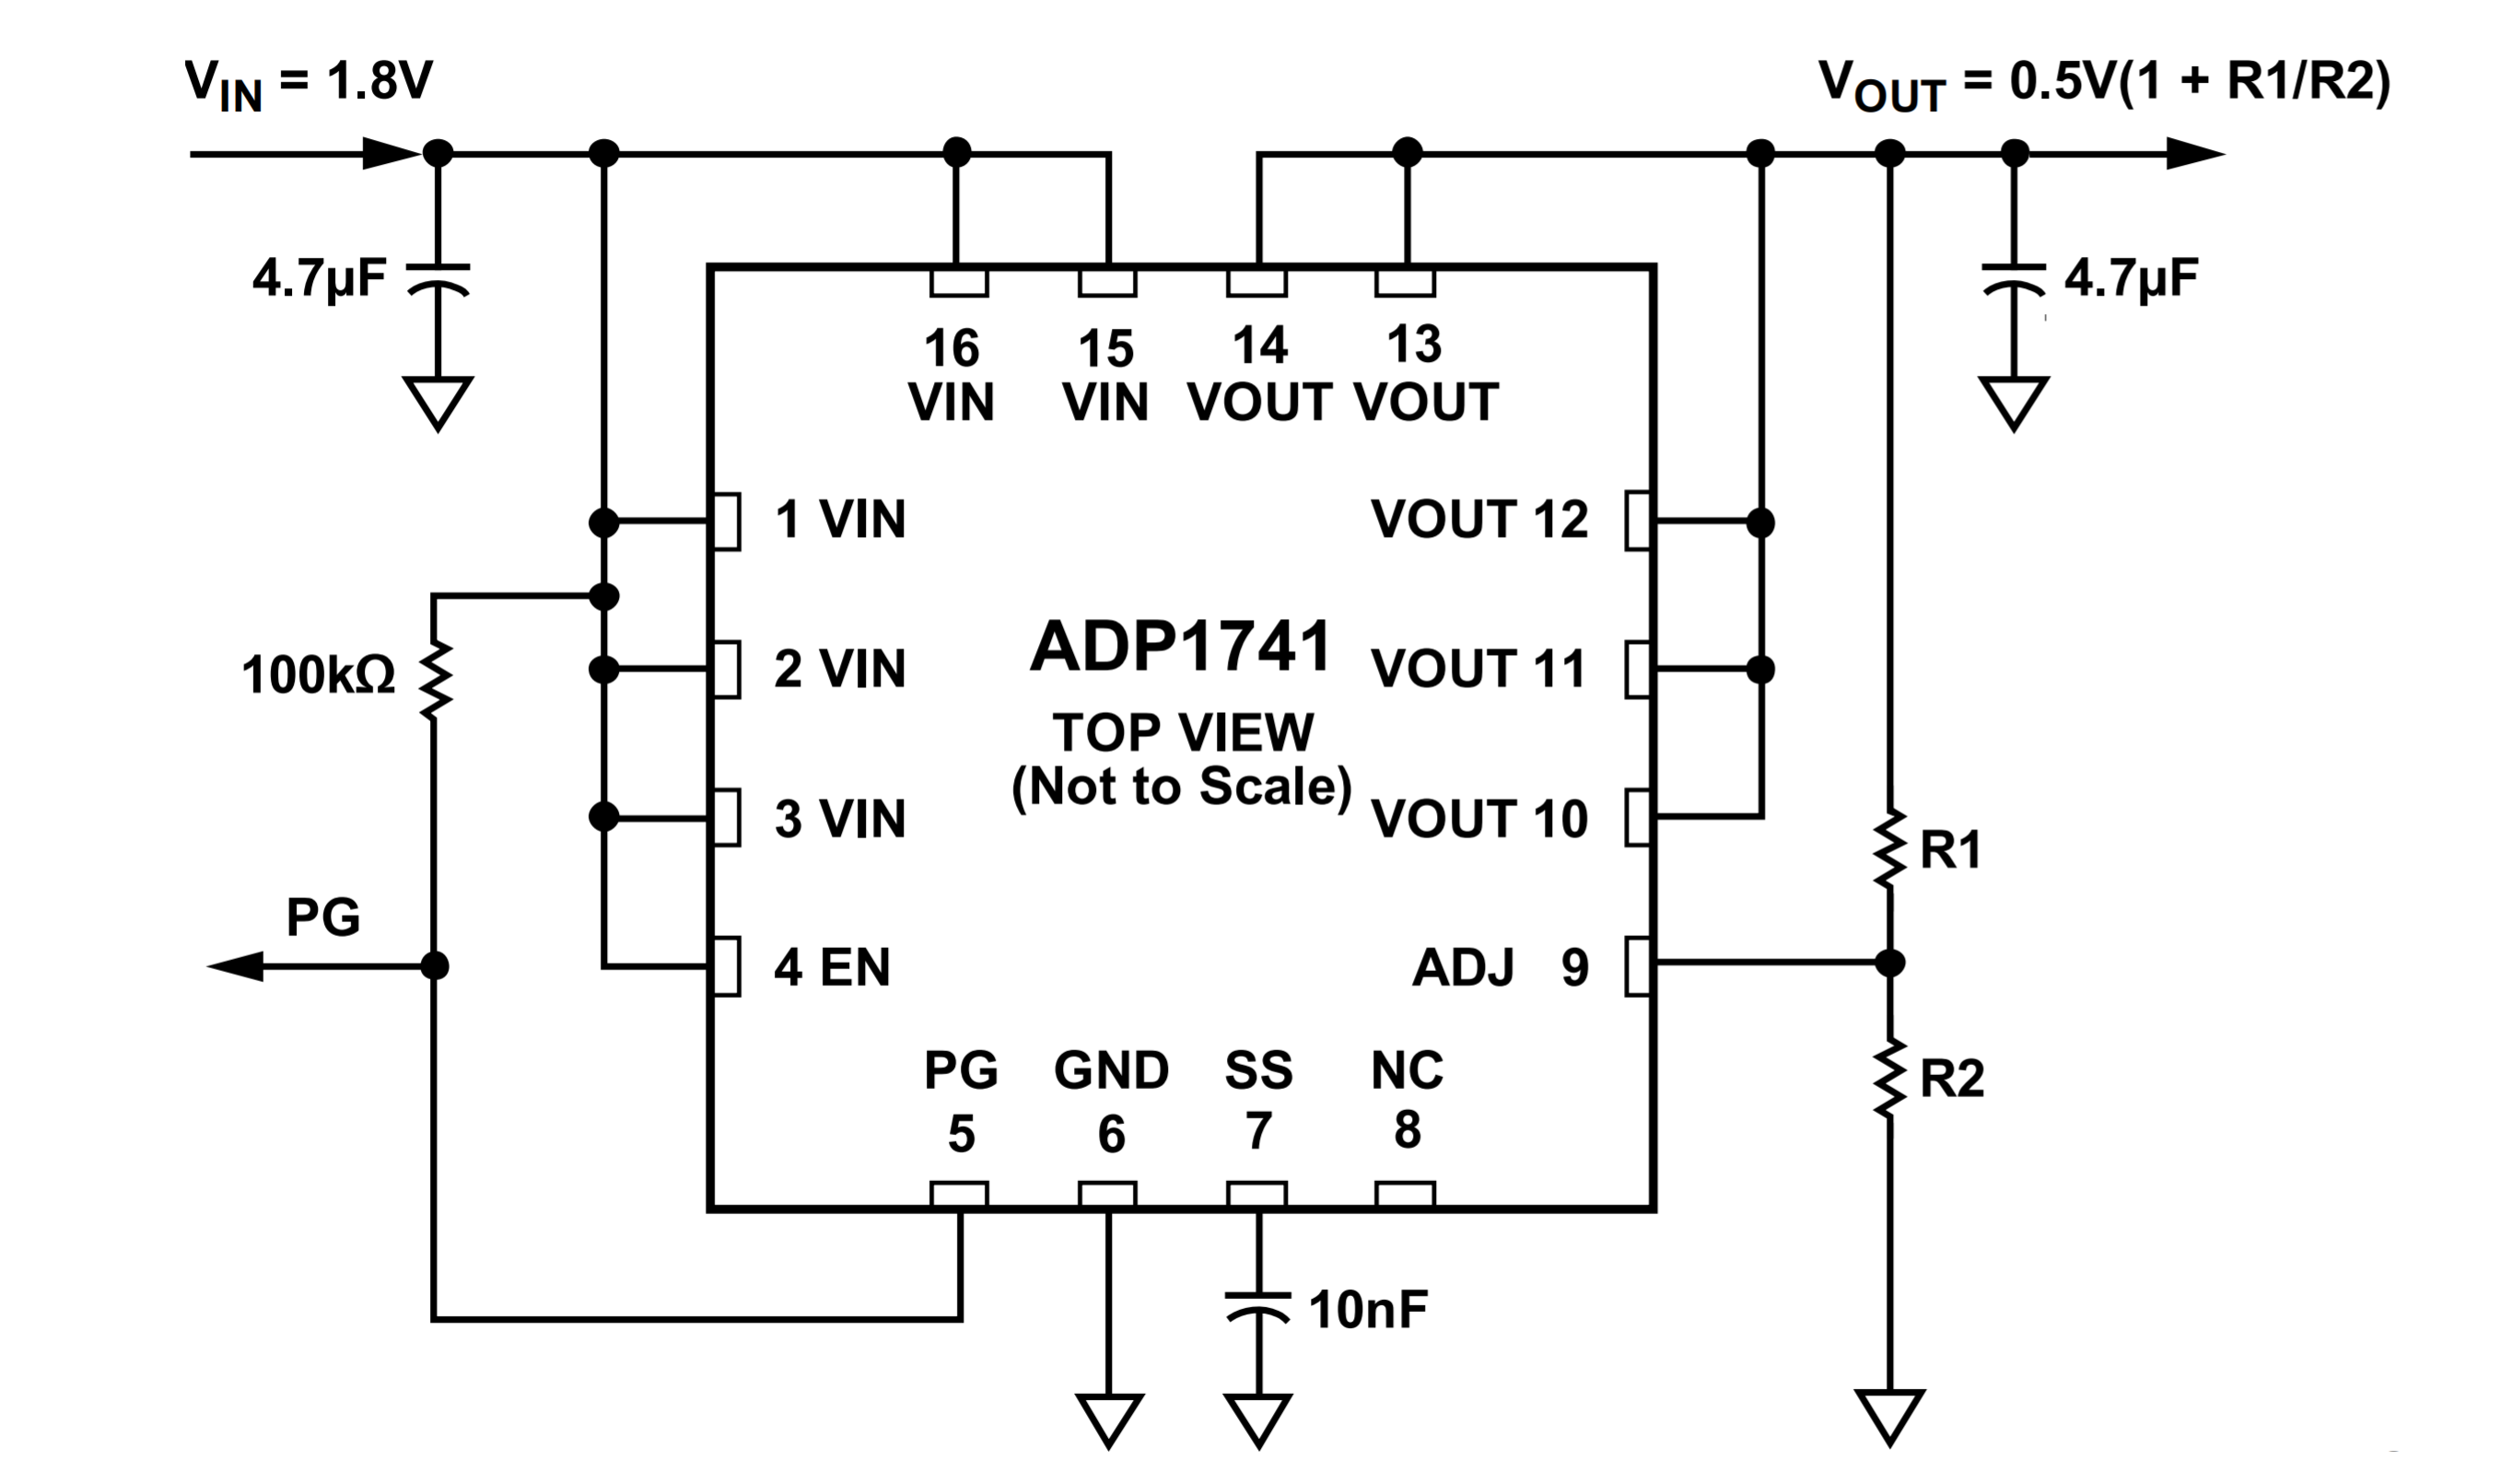
\includegraphics[width = \textwidth]{chap/04-theresa/img/schematic/adp1741_d}
	\caption{Recommended schematic of the ADP1741 voltage regulator \cite{adp1741}}
	\label{fig:adp1741}
\end{figure}

As input voltage, the \SI{3.3}{\volt} from the external power supply is provided. 

Capacitors and resistors are placed as recommended in the data sheet \cite{adp1741}(see \autoref{fig:adp1741}).

\subsubsection*{Voltage Regulator for Delay Chips}
The delay chips require a voltage level of \SI{2.5}{\volt}. As they propagate the sensitive clock signals they also need stable voltage levels. 
The number of delay chips $N$ with a maximal current draw $I_\text{m, Delay}$, which one \gls{ldo} can handle, can again be calculated as:
%todo nicefrac
\begin{align*}
	I_\text{max, LDO}                                         & > 2 \cdot N \cdot I_\text{m, Delay} \\
	\nicefrac{I_\text{max, LDO}}{(2 \cdot I_\text{m, Delay})} & > N                                 \\
	\SI{2}{\ampere} / (2\cdot \SI{0.170}{\ampere})            & > N                                 \\
	5.88                                                      & > N \quad \rightarrow N = 5
\end{align*}
Therefore, two regulators are needed to cover the 8 delay chips.
In order to keep the current draw evenly distributed among the regulators, 4 chips are assigned to one regulator respectively.

In order to set the output voltage of the regulator to \SI{2.5}{\volt}, the resistor values $R_1 = \SI{12}{\kilo \ohm}$ and $R_1 = \SI{3}{\kilo \ohm}$ are chosen (refer to \autoref{fig:adp1741} and \autoref{eq:ldo}). %todo zweimal R1

The \SI{2.5}{\volt} are also used as input for the bus transceiver which acts as a level translator. 
The current draw from this component lies in the range of \si{\micro \ampere} and can thus be neglected.

As input voltage these regulators receive the digital \SI{3.3}{\volt} from the \gls{fmc}+ connector.
The ground pins are connected to the digital ground of the \gls{pcb}.
This is important, in order to keep the analog and digital grounds and components separated.

\paragraph{Power Dissipation of the Voltage Regulators}
According to the data sheet of the ADP1741 \cite{adp1741}, the power dissipation $P_D$ of the regulator can be calculated with the input and output voltages $V_\text{IN}$ and $V_\text{OUT}$, load current $I_\text{LOAD}$ and ground current $I_\text{GND}$\footnote{difference between input and output current}:

\begin{equation}
	P_D = (V_\text{IN} - V_\text{OUT}) \cdot I_\text{LOAD} + (V_\text{IN} \cdot I_\text{GND})
\end{equation}

$I_\text{GND}$ is very small (range of \SI{}{\micro \ampere}), thus the power dissipation due to this current can be neglected.
Therefore the equation above can be simplified to:
\begin{equation}
	P_D = (V_\text{IN} - V_\text{OUT}) \cdot I_\text{LOAD}
\end{equation}

The power dissipation $P_\text{D, THA}$ of one voltage regulator for the \glspl{tha} is therefore
\begin{equation}
	P_\text{D, THA} = (\SI{3.3}{\volt} - \SI{2}{\volt}) \cdot (4 \cdot \SI{0.221}{\ampere}) = \SI{1.149}{\watt}.
\end{equation}

The power dissipation $P_\text{D, Delay}$ of one voltage regulator for the delay chips is 
\begin{equation}
	P_\text{D, Delay} = (\SI{3.3}{\volt} - \SI{2.5}{\volt}) \cdot (4 \cdot \SI{0.17}{\ampere}) = \SI{0.544}{\watt}.
\end{equation}

In order to dissipate the heat, an exposed pad is provided under the component.
This pad can be connected through vias to a (ground) plane located on the inner layers, in this way allowing to dissipate the heat through the \gls{pcb}.
Furthermore, a matrix of vias is placed underneath the component area in order to improve the heat flow.
This should be enough to handle the calculated power dissipation.
Heat sinks could be added later during operation, if the deployed method is not sufficient to dissipate the produced heat.

\clearpage
\section{Layout}
After completing the schematic capture, the following step is the \gls{pcb} layout design.
During this process, the following points need to be considered:
\begin{itemize}
	\item An appropriate \gls{pcb} substrate has to be chosen. The most important parameter of a substrate is its dielectric constant. For high-frequency circuits, a low dielectric constant is necessary.
	\item Generally, complex \glspl{pcb} consist of a number of layers. In order to be able to route all the signals, it is necessary to think about the number of layers needed. 
	\item Closely linked to the dielectric constant are the transmission lines. The geometry of these lines has to be calculated in order to meet the desired characteristic impedance (single-ended: \SI{50}{\ohm}, differential pair: \SI{100}{\ohm}). As this impedance also is defined by the dielectric constant, this step is closely linked to the selection of the substrate.
	\item Components need to be placed in a way that minimizes traces and routing. Sensitive components, like \glspl{tha} have to be placed first 
	\item Route traces, taking care that traces of the same group (e.g. clock signals distributed to the \glspl{tha}) have the same length. For sensitive signals take care that these are shielded by ground planes on the layers above and below.
	\item Placing additional structures to reduce cross-talk, \gls{emi}, etc. (via fences, stitching vias, \dots)
	\item Creating proper power distribution by placing planes at appropriate places, i.e. reducing overlapping with traces carrying signals that could induce noise on the power plane.
\end{itemize}

For better understanding, first a general overview over \gls{pcb} structures is given. 
Then the steps mentioned above are described.
\subsection*{PCB Structures Overview} \label{ssec:pcb_structs}
In this section an overview over the basic structures on a \gls{pcb} is given.
\paragraph{Traces}
A \textit{trace} is a strip of metal, which establishes an electrical connection and carries signals between two (or more) points in the horizontal plane of a \gls{pcb}. \cite{xilDecouple}

\paragraph{Planes}
\textit{Plane} denotes an uninterrupted area of metal, which covers the whole \gls{pcb} layer.
If this area only covers a part of the layer, it is called a \textit{planelet}.
These areas provide power distribution or ground across the \gls{pcb} and present an important transmission medium for the return currents\footnote{Any current that is injected into the components/boards, needs a return path, as otherwise there is no closed circuit.}. \cite{xilDecouple}

\paragraph{Vias}
A via is metal-plated hole, which is used to route a trace in vertical direction, i.e. from the \gls{pcb} outer layer to the inner layers.
They carry signals and power. Three types of vias are \cite{vias}:
\begin{itemize}
	\item Blind via: A blind via connects the surface layers with a few layers below.
	\item Buried via: A buried via only connects internal layers.
	\item Through-via: A through-via goes from one \gls{pcb} surface to another and is used to connect any layer. 
\end{itemize}
\begin{figure}[tb]
	\centering
	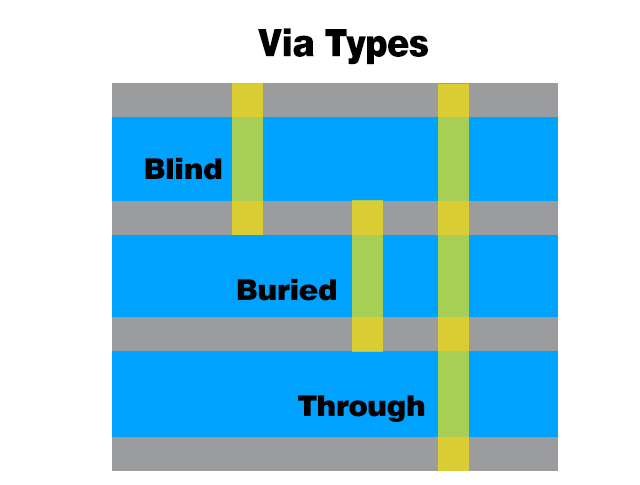
\includegraphics[width = 0.5\textwidth]{chap/04-theresa/img/pcb/vias.tikz}
	\caption[Via types]{Visualization of via types \cite{vias}}
	\label{fig:vias}
\end{figure}
In this design only blind and through vias are used.

\clearpage
\subsection{PCB Substrate Selection and Metal Layer Stackup}\label{ssec:substrate}
High-frequency transmission lines require an appropriate and very pure substrate dielectric, which needs to be selected to match the maximum frequency, the acceptable losses, and transmission lines typologies.
The Megtron6 substrate from \textit{Panasonic} is designed for high-speed/high frequency applications. 
Characteristics of this material are:
\begin{itemize}
\item Low dielectric constant: $\varepsilon_r$ = 3.61 at \SI{10}{\giga \hertz}, 3.71 at \SI{1}{\giga \hertz}
\item Low dielectric dissipation factor: 0.002 at \SI{10}{\giga \hertz}, 0.004 at \SI{1}{\giga \hertz}
\item Low transmission loss
\item High heat resistance: Decomposition temperature $\vartheta_d$ = \SI{410}{\celsius} %todo celsius is vartheta, Kelvin uses T..., right?
\end{itemize}

Another important step is deciding the number of layers. The complexity of the board implies that a lot of layers are needed in order to integrate the analog and digital signal lines, as well as the necessary power planes.
For this design a number of 16 layers is chosen.

In order to keep the analog and digital part of the \gls{pcb} separated, the top eight layers are dedicated solely to the digital signal lines and components, the bottom eight to the analog.
For shielding purposes, every second layer contains a (analog or digital) ground plane covering the whole layer.
\gls{rf} transmission lines carrying the sensitive analog signals from the detector are therefore routed on the inner layers in order to guarantee shielding from any noise or interference.
Slow control signals are routed in such way to not destroy the ground above/below the \gls{rf} lines, i.e. avoiding the area around these lines.

Lines, where time skew control needs to be very precise, are routed in inner layers. 
Due to the dielectric on both sides of the line, the electromagnetic waves propagate with lower speed, than if the signal lines would have been routed on the top layer.
The speed of the waves $V_P$ can be calculated with the speed of light $c$ and the effective dielectric constant $\varepsilon_\text{r,eff}$ as (see \cite{thierauf}):
\begin{equation}
	V_P = \frac{c}{\sqrt{\varepsilon_\text{r,eff}}}
\end{equation}
The dielectric constant of air\footnote{1.00059 at room temperature (\SI{25}{\degreeCelsius}) \cite{dielectric}} is approximately 1, meaning the effective dielectric constant for waves propagating on the top layers is smaller, than the one for waves propagating in the inner layers where they are surrounded by the substrate.
According to the equation above, this also results in a higher propagation speed. 
Time skew control can be handled more easily for slower waves, meaning for lines where the arrival time of the signals should be matched as precise as possible, propagation in the inner layers is necessary.

Filtered voltage from the power supplies is propagated through vias to the inner layers, from where the levels are distributed to the respective components, either by connected plane or single traces.

%https://industrial.panasonic.com/content/data/EM/PDF/ipcdatasheet\_R-5775.pdf

\clearpage
\subsection{Transmission Lines}
Transmission lines guide electromagnetic waves from one point to another with a well-defined impedance. 
They have a characteristic impedance which is determined by parameters like width of the trace, separation from ground plane, etc.  
A mismatch can lead to reflections and damping of the \gls{rf} signals.
For single-ended signals the waveguide characteristic impedance for the front-end sampling card is \SI{50}{\ohm}, for differential pairs \SI{100}{\ohm}.
The impedance has to be matched especially for sensitive, high-speed signals, e.g. clock signals. 
Proper calculation of the geometrical parameters is therefore very important to ensure signal integrity and reduce reflection and damping. 

Formulas to calculate the characteristic impedance are quite complex (see \autoref{app:waveguides} in appendix) and not easy to solve.
To make the design of transmission lines easier, specific tools are used for quick calculations of the geometric values needed for impedance matching.
For this design, the \textit{Si9000e} tool for modeling \gls{pcb} transmission lines from \textit{Polar} is used to calculate the necessary trace widths, trace separations, etc.
A screenshot of the Polaris tool, showing the geometry of a coplanar waveguide is shown in \autoref{fig:polaris}. Note that the labels used in the tool to indicate the different geometry parameters are different from the ones used in this thesis.
\begin{figure}[tb]
	\centering
	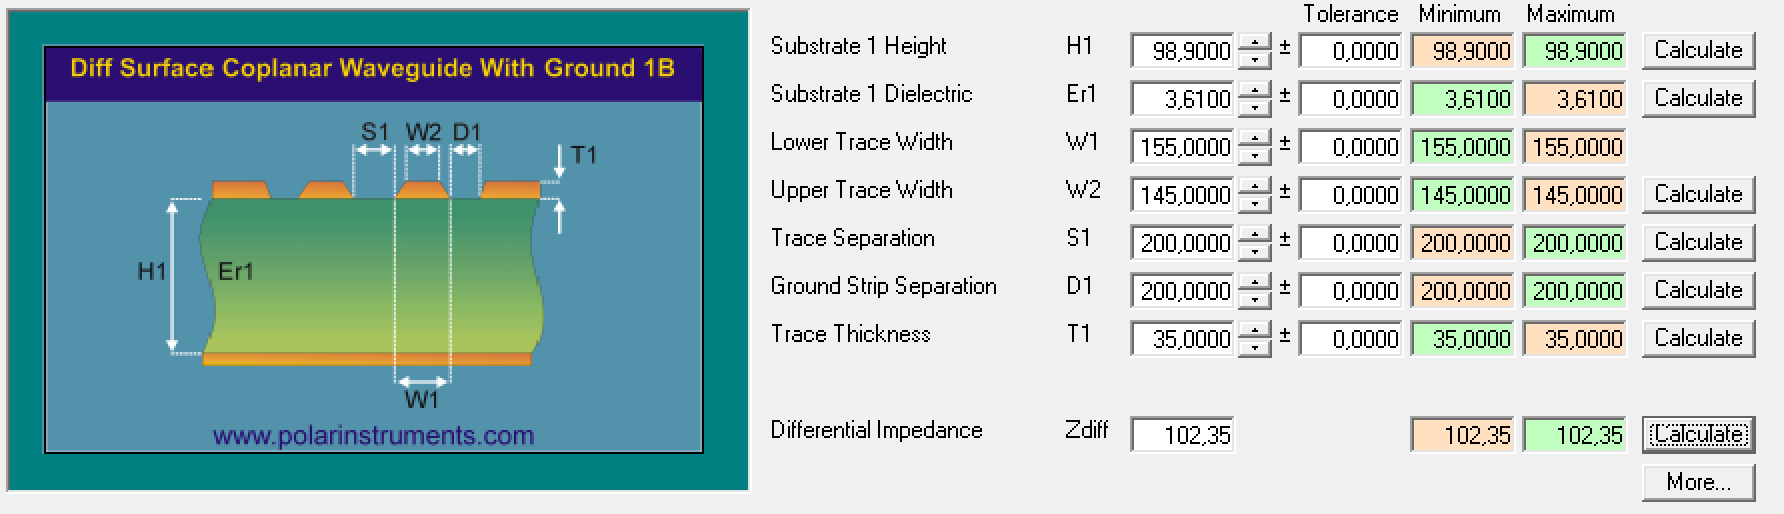
\includegraphics[width = \textwidth]{chap/04-theresa/img/polaris}
	\caption[Screenshot of the \textit{Polar Si9000e}]{Screenshot of the \textit{Polar Si9000e} tool for modeling \gls{pcb} transmission lines, showing calculation of characteristic impedance of a coplanar waveguide}
	\label{fig:polaris}
\end{figure}

As there are a lot of parameters which can be tuned, as a starting point the geometrical parameters of the \gls{kapture} \gls{pcb} design are applied. 
These were carefully designed for optimal transmission line geometry.
However, the substrate used in the \gls{kapture} system, has a different dielectric constant than the Megtron6 substrate selected for the new design. 
Therefore, the impedance has to be recalculated. 
For the results, a deviation of 10\% from the ideal \SI{50}{\ohm} and \SI{100}{\ohm} is still regarded as acceptable, as tolerances during manufacturing need to be considered.

Three types of transmission lines have been designed for this layout:
\begin{itemize}
	\item Surface coplanar waveguide with ground layer for analog input to the \glspl{tha} 
	\item Differential surface coplanar waveguide with ground layer for output from the delay chips to the \glspl{tha}
	\item Symmetrical differential coplanar waveguide for clock signals and signals coming from the \glspl{tha}
\end{itemize}
These waveguide types and the respective geometric dimensions calculated with the \textit{Si9000e} tool are presented.

\clearpage
\paragraph{Surface Coplanar Waveguide with Ground}
The surface coplanar waveguide has the geometry shown in \autoref{fig:microstrip_geometry}.
The single trace of thickness $t$ and width $a$ lies between two ground planes on a dielectric of thickness $h$ and the effective dielectric constant $\varepsilon_r$.
Another ground plane is located at the bottom of the dielectric.
Separation between trace and ground plane is defined as $(b-a)/2 := d$. 

\begin{figure}[H]
	\centering
	\includegraphics[width = \textwidth]{chap/04-theresa/img/TL/cw.tikz}
	\caption{Coplanar Waveguide with ground plane}
	\label{fig:microstrip_geometry}
\end{figure}

To have a first starting point of the dimensions of the parameters, the following widths are taken from the \gls{kapture} board:
\begin{itemize}
	\item $a = \SI{213}{\micro \meter}$
	\item $d = \SI{250}{\micro \meter}$
\end{itemize}
In the \textit{Si9000e} tool, an upper and a lower trace width can be specified taking into account the etching process during manufacturing.
The exact production parameters are not known, therefore there is no knowledge about the exact upper trace width.
Therefore, for the calculation of the characteristic impedance the upper and lower trace widths are assumed to be of the same value.
The influence of the variation of the upper trace width is simulated with the tool in order to give an estimation for the characteristic impedance to be expected.
The thickness $t$ of the trace and the thickness $h$ of the dielectric is defined by the used substrate.
For Megtron6 it is 
\begin{itemize}
	\item $t = \SI{30}{\micro \meter}$
	\item $h = \SI{100}{\micro \meter}$.
\end{itemize}
With all these parameters, the value for the characteristic impedance is calculated to $Z_o = \SI{47.33}{\ohm}$.
This lies well in the 10\% tolerance range of \SIrange{45}{55}{\ohm}. 

According to the data sheet of the Megtron6 substrate, the dielectric constant $\varepsilon_r$ changes over frequency (see \autoref{ssec:substrate}).
As the dielectric constant $\varepsilon_r$ of the Megtron6 substrate varies between 3.61 and 3.71 depending on the frequency, the effect of the changing $\varepsilon_r$ should also be studied. 
The \textit{Si9000e} tool provides the possibility to simulate the characteristic impedance versus a changing parameter.

In \autoref{fig:surf_dk} the characteristic impedance $Z_o$ is plotted against $\varepsilon_r$.
It can be seen that with higher effective dielectric constant the characteristic impedance decreases.
The lowest values lies around \SI{47}{\ohm}, a change of \SI{0.7}{\percent}, which is still inside the 10\% tolerance range.

Furthermore, the effect of changing the trace width on $Z_o$ is studied and shown in \autoref{fig:surf_w1}.
This plot shows that for best matching of the impedance a trace thickness of around \SI{200}{\micro \meter} is the best choice.
This result however does not take into account the real upper trace width.

For an estimation of the effect of the upper trace width on the impedance, a constant lower trace width of \SI{213}{\micro \meter} and $\varepsilon_r = 3.61$ is assumed, while varying the upper trace width from \SIrange{183}{213}{\micro \meter}.
The result is shown in \autoref{fig:surf_w2}.
With decreasing width the characteristic impedance approaches the desired \SI{50}{\ohm}.

\begin{figure}[tb]
	\centering
	\includegraphics[width = \textwidth, height = 0.4\textwidth]{chap/04-theresa/img/TL/surf/surf_dk.tikz}
	\caption[CWG, $Z_o$ vs $\varepsilon_r$]{Characteristic impedance $Z_o$ of a coplanar waveguide versus dielectric constant $\varepsilon_r$ assuming $a = \SI{213}{\micro \meter}$}
	\label{fig:surf_dk}
\end{figure}

\begin{figure}[tb]
	\centering
	\includegraphics[width=\textwidth, height = 0.4\textwidth]{chap/04-theresa/img/TL/surf/surf_w1}
	\caption[CWG, $Z_o$ vs. $a$]{$Z_o$ of a coplanar waveguide vs. lower trace thickness $a$, assuming $\varepsilon_r = 3.61$}
	\label{fig:surf_w1}
\end{figure}

\begin{figure}[tb]
	\centering
	\includegraphics[width=\textwidth, height = 0.4\textwidth]{chap/04-theresa/img/TL/surf/surf_w2}
	\caption[CWG, $Z_o$ vs. upper trace width]{$Z_o$ of a coplanar waveguide vs. upper trace thickness}
	\label{fig:surf_w2}
\end{figure}

\autoref{fig:surf_loss} shows the calculated attenuation (combination of conductor and dielectric loss) of the coplanar waveguide with the given geometries over a frequency range \SIrange{0.1}{100}{\GHz}. 
This attenuation was calculated for the trace length of \SI{10}{\mm}, higher than the actually routed trace.
As can be derived from the plot, the attenuation lies well below \SI{1}{\decibel}, therefore ensuring high bandwidth of the trace.
\begin{figure}[tb]
	\centering
	\includegraphics[width=\textwidth, height = 0.4\textwidth]{chap/04-theresa/img/TL/surf/loss}
	\caption[Attenuation CPWG for \SI{10}{\mm}]{Attenuation per trace length of the surface coplanar waveguide over frequency simulated for trace length of \SI{10}{\mm}}
	\label{fig:surf_loss}
\end{figure}

\clearpage
\paragraph{Differential Pairs on Surface}
The geometry of the differential surface is similar to the waveguide type before, with the difference of having a pair of traces instead of one single trace (see \autopageref{fig:eccw_geometry}).
The characteristic differential impedance $Z_\text{diff}$ of this transmission line type is determined by the trace width $w$, the trace separation $s$, the trace-to-ground-separation $d$, the thickness of the trace $t$ and thickness of the dielectric $h$.

\begin{figure}[H]
	\centering
	\includegraphics[width = \textwidth]{chap/04-theresa/img/TL/eccw.tikz}
	\caption{Edge-coupled differential coplanar waveguide}
	\label{fig:eccw_geometry}
\end{figure}

The parameters $t$ and $h$ have the same value, as for the coplanar waveguide described below.
For the other parameters first the following values are assumed:
\begin{itemize}
	\item Trace width $w = \SI{180}{\micro \meter}$ 
	\item Trace separation $s = \SI{150}{\micro \meter}$
	\item Trace-to-ground separation $d = \SI{600}{\micro \meter}$
\end{itemize}
For these parameters and an $\varepsilon_r = 3.61$ an impedance of \SI{92.35}{\ohm} is calculated with the \textit{Si9000e} tool.
This is still inside the tolerance band, but can potentially be improved.
The lower trace width is chosen as changing parameter in order to improve the characteristic impedance.

In \autoref{fig:surf_diff_w1} a the characteristic impedance $Z_\text{diff}$ is plotted against the trace width\footnote{Assuming lower and upper trace width are equal.}. 
The impedance $Z_\text{diff}$ lies around \SI{100}{\ohm} for a trace width $w \approx$\SI{155}{\micro \meter}.

\begin{figure}[tb]
	\centering
	\includegraphics[width=\textwidth, height = 0.4\textwidth]{chap/04-theresa/img/TL/surf_diff/surf_diff_w1}
	\caption[DCWG, $Z_\text{diff}$ vs. $w$]{$Z_\text{diff}$ of an edge-coupled differential coplanar waveguide vs. lower trace width $w$, assuming $\varepsilon_r = 3.61$}
	\label{fig:surf_diff_w1}
\end{figure}

Setting the width to \SI{155}{\micro \meter} indeed gives an impedance of $Z_\text{diff} = \SI{99.37}{\ohm}$.
The influence of the changing dielectric constant $\varepsilon_r$ is studied in this case as well (see \autoref{fig:surf_diff_dk}). 
At the maximal value of $\varepsilon_r = 3.71$, the impedance lies around \SI{98.4}{\ohm} corresponding to a change of \SI{0.88}{\percent} compared to the value at $\varepsilon_r = 3.61$. 

\begin{figure}[tb]
	\centering
	\includegraphics[width = \textwidth, height = 0.4\textwidth]{chap/04-theresa/img/TL/surf_diff/surf_diff_dk}
	\caption[DCWG, $Z_\text{diff}$ vs. $\varepsilon_r$]{$Z_\text{diff}$ of an edge-coupled differential coplanar waveguide vs. dielectric constant $\varepsilon_r$}
	\label{fig:surf_diff_dk}
\end{figure}


Furthermore, assuming $\varepsilon_r = 3.61$ and a lower trace width $w = \SI{155}{\micro \meter}$, the impedance over a varying upper trace width is plotted in \autoref{fig:surf_diff_w2}.

\begin{figure}[tb]
	\centering
	\includegraphics[width = \textwidth, height = 0.4\textwidth]{chap/04-theresa/img/TL/surf_diff/surf_diff_w2}
	\caption[DCWG, $Z_\text{diff}$ vs. upper trace width]{$Z_\text{diff}$ of an edge-coupled differential coplanar waveguide vs. upper trace width, assuming lower trace width $w = \SI{155}{\micro \meter}$ and$\varepsilon_r = 3.61$}
	\label{fig:surf_diff_w2}
\end{figure}

\autoref{fig:surf_diff_loss} shows the calculated attenuation (combination of conductor and dielectric loss) of the coplanar waveguide with the given geometries over a frequency range \SIrange{0.1}{10}{\GHz}.
This range is interesting as the signals propagated on these lines (e.g. clock signals) do not extend \SI{10}{\GHz}.
This attenuation was calculated for the trace length of \SI{50}{\mm}, an estimation of the maximal length of such lines.
As can be derived from the plot, the attenuation lies under \SI{2}{\decibel}, which is an acceptable result for the design.

\begin{figure}[bhbh]
	\centering
	\includegraphics[width=\textwidth, height = 0.4\textwidth]{chap/04-theresa/img/TL/surf_diff/loss}
	\caption[Attenuation DCWG for \SI{200}{\mm}]{Attenuation per trace length of the surface differential coplanar waveguide over frequency simulated for trace length of \SI{50}{\mm}}
	\label{fig:surf_diff_loss}
\end{figure}

\clearpage

\paragraph{Differential Pairs between Layers}
The analog signals from the \glspl{tha}, as well as the clock signals, are propagated through differential pair traces on the inner layers of the \gls{pcb}. 
This forms a symmetrical differential coplanar waveguide as seen in \autoref{fig:docw_d1}.
The impedance of this waveguide type depends on the trace width $w$, the trace separation $s$, the trace-to-ground separation $d$, the thickness $t$ of the trace, as well as the thickness of the dielectrics $h_1$ and $h_2$ and their respective dielectric constant $\varepsilon_1$ and $\varepsilon_2$.

\begin{figure}[H]
	\centering
	\includegraphics[width = \textwidth]{chap/04-theresa/img/TL/docw.tikz}
	\caption{Symmetrical differential coplanar waveguide}
	\label{fig:docw_d1}
\end{figure}

The parameters are assumed as
\begin{itemize}
	\item Trace width $w = \SI{88}{\micro \meter}$ 
	\item Trace separation $s = \SI{150}{\micro \meter}$
	\item Trace-to-ground separation $d = \SI{250}{\micro \meter}$
\end{itemize}
The thickness of the dielectrics is $h_1 = h_2 = \SI{150}{\micro \meter}$  and the dielectric constant is equal for both ($\varepsilon_1 = \varepsilon_2 = \varepsilon_r = 3.61$).
With these parameters the impedance is calculated as $Z_\text{diff} = \SI{90.40}{\ohm}$.
In \autoref{fig:off_diff_w1} $Z_\text{diff}$ is plotted against the trace width $w$ (assuming upper trace width equal to $w$). It can be seen, that in order to improve the impedance, one should decrease the trace width. 
Due to the manufacturing technology the minimal trace width possible is \SI{88}{\micro \meter}. 
Therefore this option is not feasible.

\begin{figure}[tb]
	\centering
	\includegraphics[width = \textwidth, height = 0.4\textwidth]{chap/04-theresa/img/TL/off_diff/off_diff_w1}
	\caption[SCWG, $Z_\text{diff}$ vs. $w$]{$Z_\text{diff}$ of a symmetrical differential coplanar waveguide vs. lower trace width $w$, assuming upper trace width equals to $w$}
	\label{fig:off_diff_w1}
\end{figure}

Keeping the trace width constant at $w = \SI{88}{\micro \meter}$, the trace separation could also be changed.
\autoref{fig:off_diff_s1} shows $Z_\text{diff}$ plotted against the trace separation $s$.
It can be seen that $Z_\text{diff}$ does not change significantly over a large range of $s$.
For a trace separation of around \SI{300}{\micro \meter} (more than 3 times larger than the trace width itself), $Z_\text{diff}$ is approximately $\SI{94}{\ohm}$ and is not significantly improved.
Taking this, as well as the available space on the board into consideration, the parameters are left as they are.  
\begin{figure}[tb]
	\centering
	\includegraphics[width = \textwidth, height = 0.4\textwidth]{chap/04-theresa/img/TL/off_diff/off_diff_s1}
	\caption[SCWG, $Z_\text{diff}$ vs. $s$]{$Z_\text{diff}$ of a symmetrical differential coplanar waveguide vs. trace separation $s$, assuming trace width $w = \SI{88}{\micro \meter}$}
	\label{fig:off_diff_s1}
\end{figure}

The influence of the dielectric constant $\varepsilon_r$ is shown in \autoref{fig:off_diff_dk}. 
$Z_\text{diff}$ decreases with higher value of $\varepsilon_r$ and even gets below \SI{90}{\ohm}, exceeding the \SI{10}{\percent} tolerance.
However, the upper trace width has to be considered as well, which is in any case smaller than the lower trace width due to the etching process during manufacturing.
As \autoref{fig:off_diff_w2} shows, the impedance is potentially higher than calculated by assuming both width equal. Therefore the impedance can still be regarded as falling into the tolerance band.
\begin{figure}[tb]
	\centering
	\includegraphics[width = \textwidth, height = 0.4\textwidth]{chap/04-theresa/img/TL/off_diff/off_diff_dk}
	\caption[SCWG, $Z_\text{diff}$ vs. $\varepsilon_r$]{$Z_\text{diff}$ symmetrical differential coplanar waveguide vs. dielectric constant $\varepsilon_r$, assuming lower trace width $w = \SI{88}{\micro \meter}$ and $\varepsilon_r = 3.61$}
	\label{fig:off_diff_dk}
\end{figure}


\begin{figure}[tb]
	\centering
	\includegraphics[width = \textwidth, height = 0.4\textwidth]{chap/04-theresa/img/TL/off_diff/off_diff_w2}
	\caption[SCWG, $Z_\text{diff}$ vs. upper trace width]{$Z_\text{diff}$ Symmetrical differential coplanar waveguide vs. upper trace width, assuming lower trace width $w = \SI{88}{\micro \meter}$ and $\varepsilon_r = 3.61$}
	\label{fig:off_diff_w2}
\end{figure}

\autoref{fig:off_diff_loss} shows the calculated attenuation (combination of conductor- and dielectric-loss) of the coplanar waveguide with the given geometries over a frequency range \SIrange{0.1}{2}{\GHz}. 
This attenuation has been calculated for the trace length of \SI{200}{\mm}, an upper estimate of the length of the traces carrying the output signal from the \glspl{tha} to the connector.
As can be derived from the plot, the attenuation reaches up to \SI{4}{\decibel}.
Considering the length of the traces, this is an expected result. 
The traces need therefore to be routed in the lowest noise conditions possible, i.e. through shielding by ground layers and placing via fences around the trace, to ensure that the signal under study is propagated correctly to the connectors.

During characterization the %todo hier fehlt was


\begin{figure}[tb]
	\centering
	\includegraphics[width = \textwidth, height = 0.4\textwidth]{chap/04-theresa/img/TL/off_diff/loss}
	\caption[SCWG]{Attenuation per trace length of the symmetrical differential coplanar waveguide over frequency simulated for trace length of \SI{200}{\mm}}
	\label{fig:off_diff_loss}
\end{figure}

\clearpage
\subsection{Component Placement and Routing}
For the placement and routing of the components many steps need to be considered.

At the beginning, the separation of the analog and digital grounds has to be taken care of. 
Due to the complexity of the board, the respective grounds need to cover the whole plane. 
Therefore, in order to guarantee a full separation without any interference between the two parts, the \gls{pcb} is split into two parts.
The topside part is dedicated to the digital components and the routing of digital signal. 
These layers cover the clocking distribution as well as the slow control signal paths leading from the \gls{fpga} to the respective components.
The bottomside of the \gls{pcb} is dedicated to the analog components and integrates the analog signal paths coming from the \glspl{tha}.

Closely linked to the structuring of the overall \gls{pcb} is the number of stacked-up metal layers used.
In order to integrate all necessary signals and power planes, 16 layers in total are used.
The topside 8 layers are therefore used for the digital part, the other 8 for the analog.
For shielding purposes and to guarantee smallest possible signal return path for the transmission lines, layers carrying signal paths are ``sandwiched'' between two ground layers.

Some signals need to be routed from top layer to bottom and vice versa by through vias. 
In order to maintain the separation between analog and digital parts in such cases, a sufficient isolation between the via and the surrounding (ground-) plane has to be ensured.

At some point, the analog and digital grounds need to be connected together. 
As mentioned in \autoref{sec:schematics}, these connections are deployed by placing ferrite beads at each \gls{tha} connecting analog and digital grounds.
This way, any noise coming from the digital ground is compensated. 
\gls{rf} filtering at the \gls{tha} is placed in the same manner, in order to mitigate any noise which could interfere with the sensitive analog signal.

As they are sensitive to interference, analog components should be placed first in order to minimize the routing paths, therefore reducing additional inductance and possible interference due to longer traces.
Also the transmission lines carrying sensitive analog signals should be routed first, in order to define the further routing of other signal paths, e.g. slow control signals. 
These transmission lines should be separated from digital signal paths as much as possible in order to reduce cross-talk between the lines. 

Routing the transmission lines should be done with time skew control in mind. 
This is especially necessary for the outputs leading from \glspl{tha} to the RFMC connector. 
Due to the asymmetric position of the connector on the board, if the \gls{tha} component outputs would be connected directly to the connector, the signal paths would vary significantly between components.
This would introduce a significant time skew between the lines.
Therefore, to account for this problem, signal paths coming from the closest \glspl{tha} need to be made longer.
This is achieved by routing the the traces in patterns called ``accordions'', which allow for prolonging the trace length in a compact way.
An example for such accordions is shown in \autoref{fig:accordion}.
\begin{figure}[tb]
	\centering
	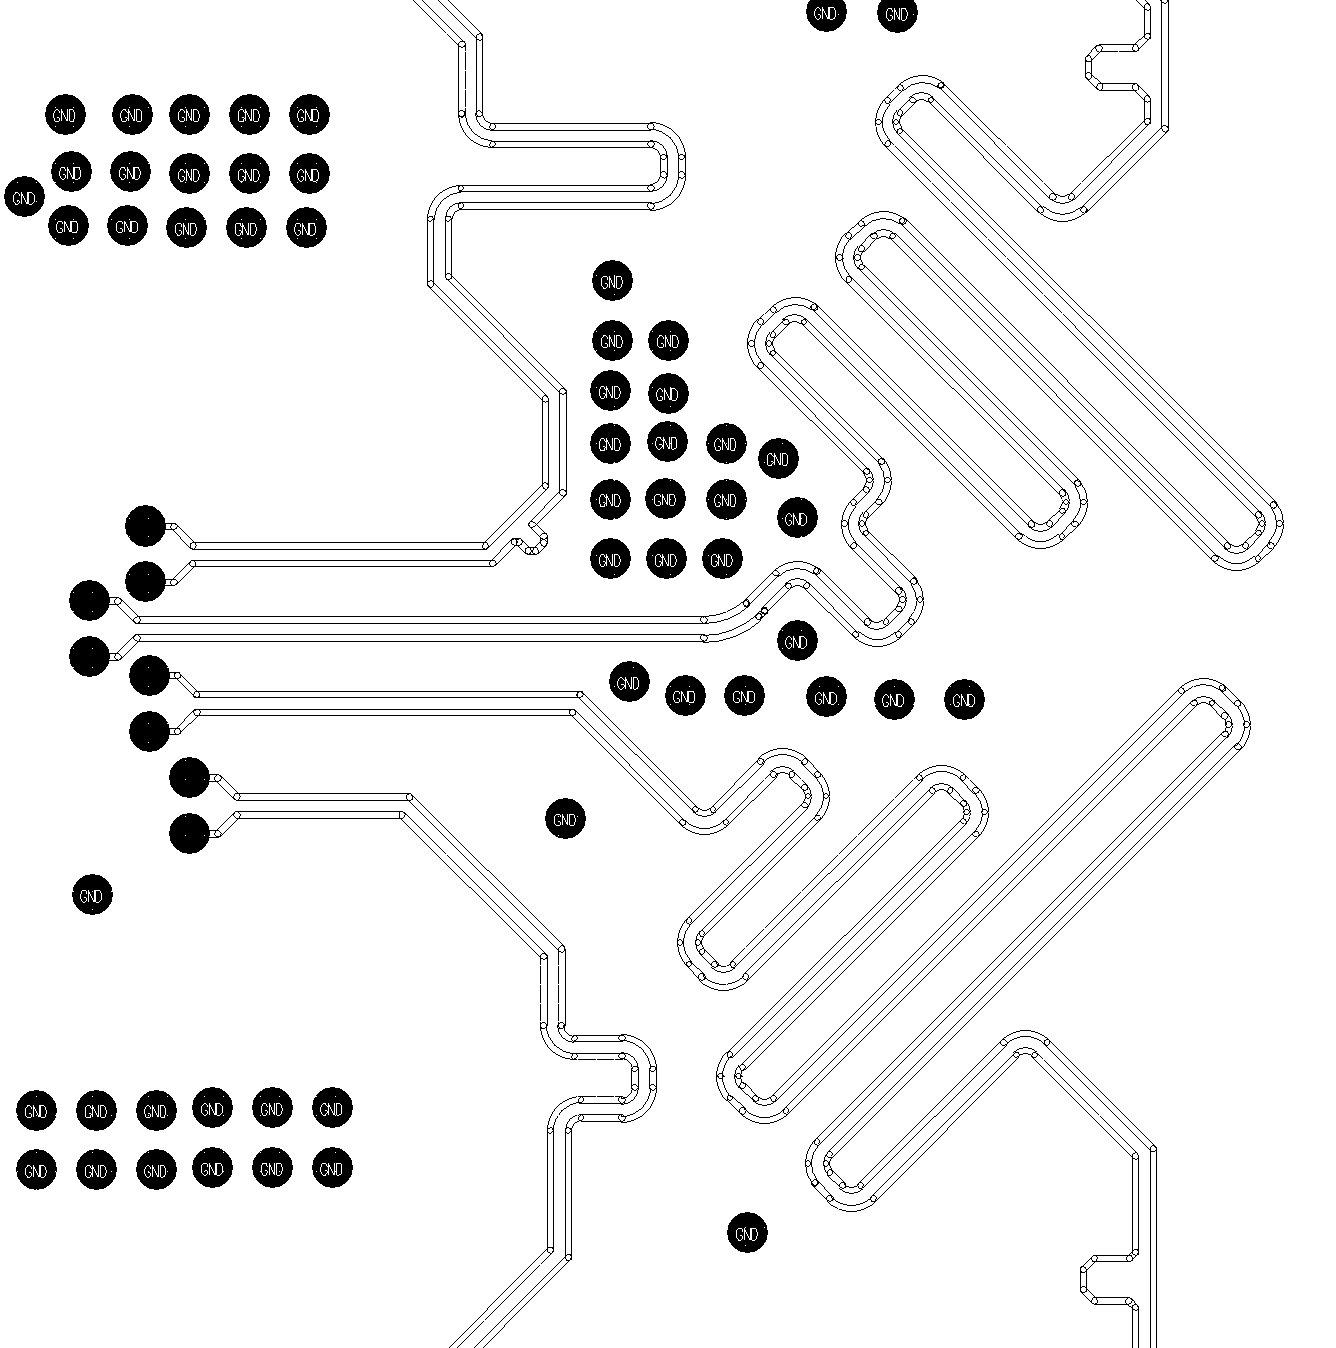
\includegraphics[width = 0.6\textwidth]{chap/04-theresa/img/pcb/accordion}
	\caption[Trace accordions]{Example for trace accordions which are used to enlarge the trace length when little space is available}
	\label{fig:accordion}
\end{figure}

To achieve high signal integrity, ``via-fences'' are placed next to the traces carrying analog signals. 
These consist of via holes connected to analog ground, placed close enough together to form a barrier for electromagnetic wave propagation. 
This forms a shield against any electromagnetic interference originating from other components on the board.
Furthermore, via-fences act as a barrier for the signal too, therefore guiding it on the desired path and limiting it to its respective area.
 \begin{figure}[tb]
 	\centering
 	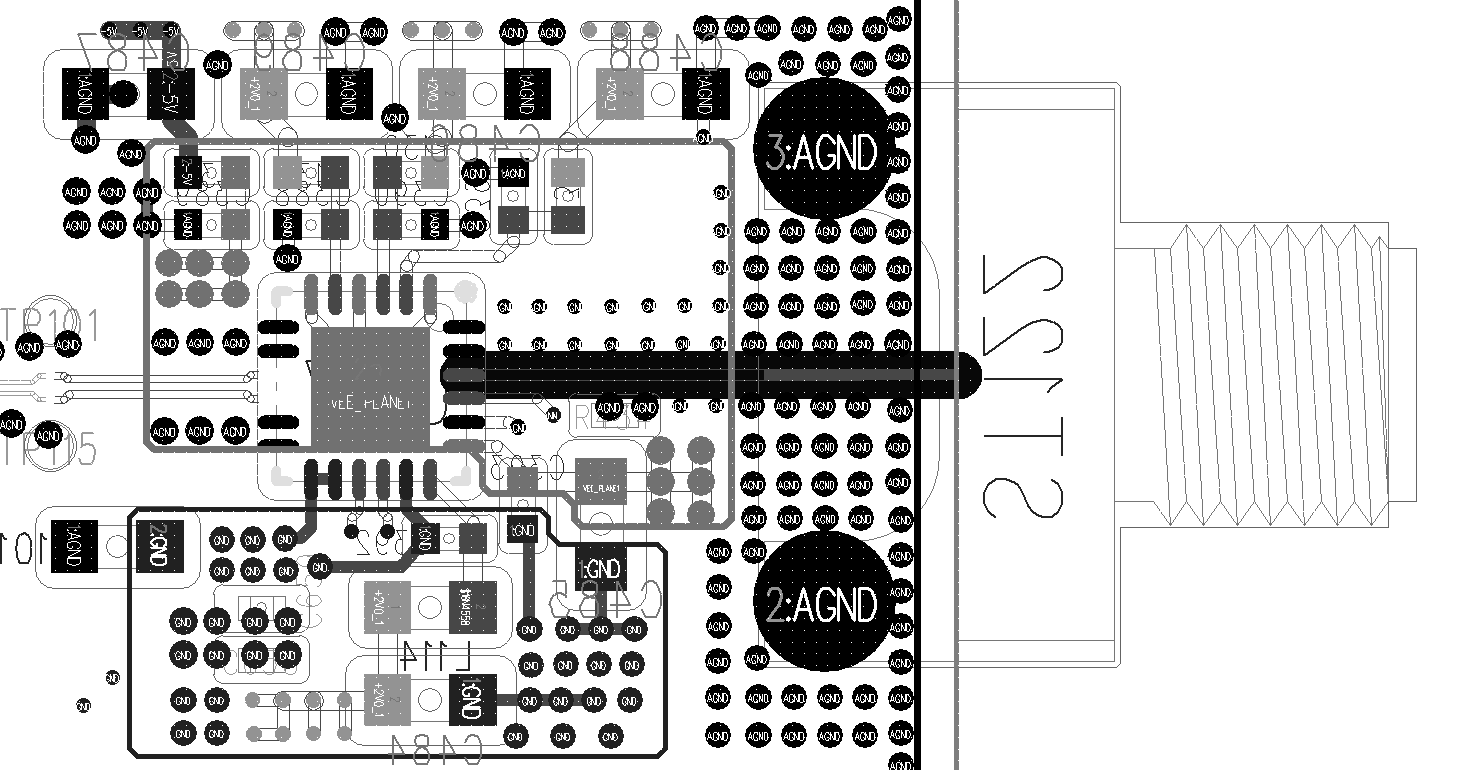
\includegraphics[width = 0.8\textwidth]{chap/04-theresa/img/pcb/tha_pcb}
 	\caption[THA layout]{Layout of the THA, showing stitching vias and RF filtering components for low noise conditions}
 	\label{fig:stitch}
 \end{figure}

\autoref{fig:sampling_card} shows the 3D model of the final design of the sampling card.
On the top side of the board (\autoref{fig:pcb_front}), the digital components, signals and clock distribution are placed. 
The clock distribution is placed on the bottom, as close as possible to the \glspl{tha}, with the main \gls{pll} in the middle.
Two \glspl{pll}, providing the high frequency clock necessary for the data converters in the \gls{fpga}, are placed close to the main \gls{pll}.
Furthermore, the \gls{fmc}+ connector is located on the top, in order to connect the board with the \gls{fpga} and to provide the slow-control signals.

On the bottom side of the board (\autoref{fig:pcb_back}), the analog components, i.e. the \glspl{tha} and analog voltage regulators are placed. 
The output of the \glspl{tha} is propagated to the \gls{rf} connector (on the left in \autoref{fig:pcb_back}), which propagates the signal to the \gls{fpga}. 
To propagate test signals from the \glspl{dac} on the \gls{fpga}, the connector on the right is used.
The small connector on the top propagates the clock signal, coming from the high-frequency \glspl{pll}, to the data converters.

\begin{figure}[tb]
	\centering
	\begin{subfigure}{\textwidth}
		\centering
		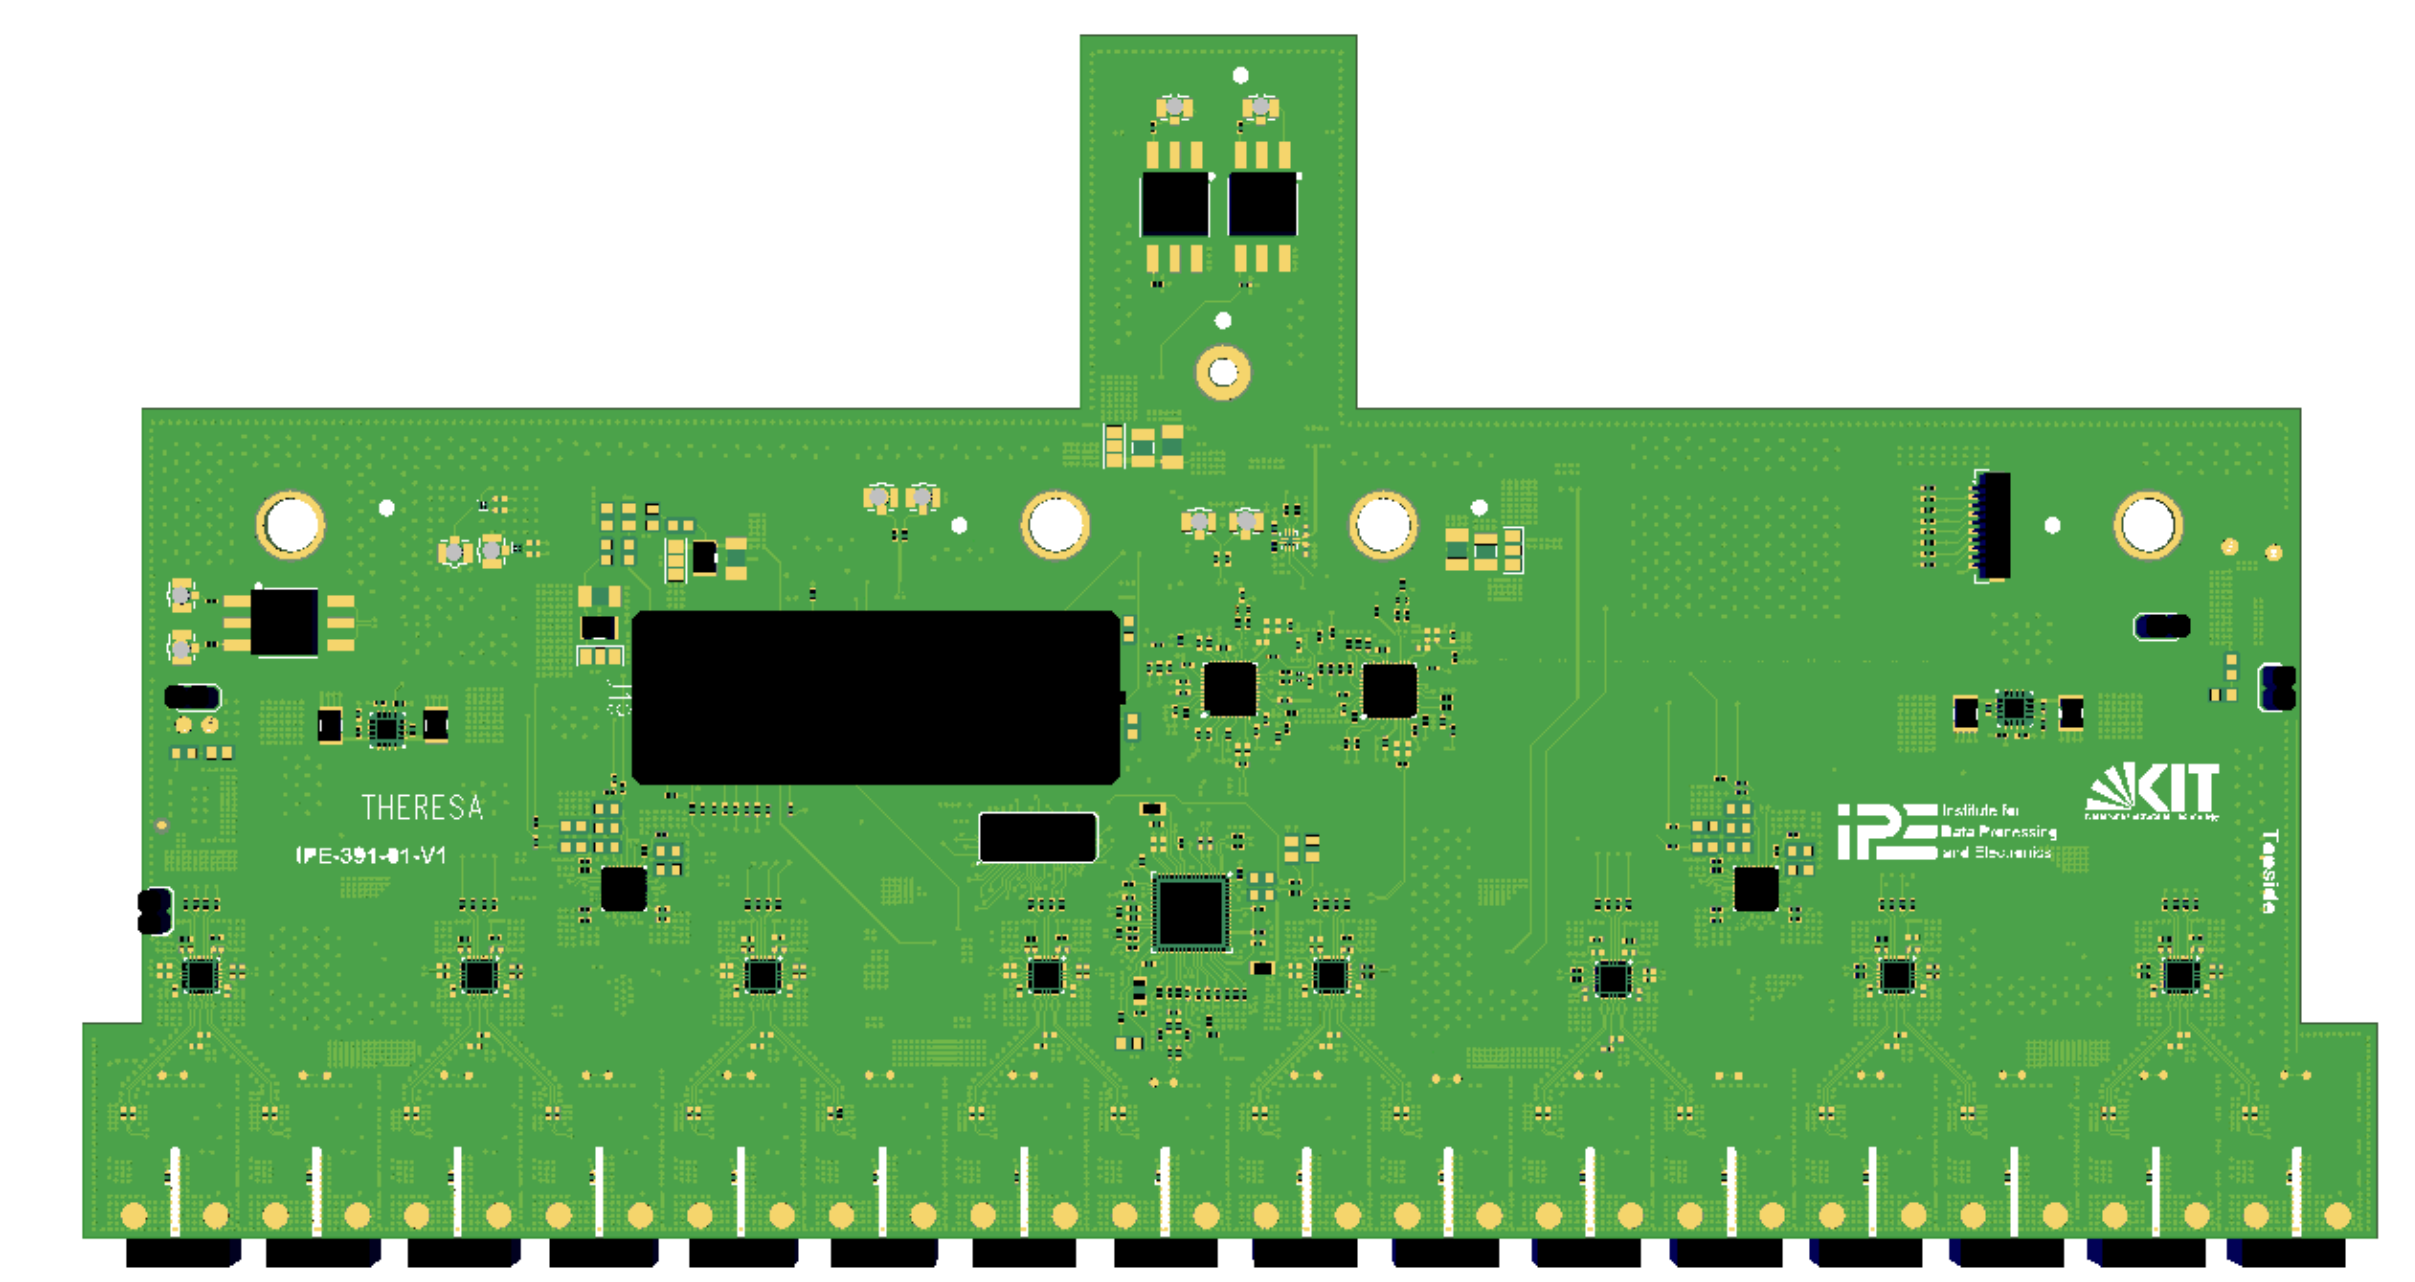
\includegraphics[width=0.85\textwidth]{chap/04-theresa/img/pcb/front_2}  
		\caption{Top side}
		\label{fig:pcb_front}
	\end{subfigure}
	\begin{subfigure}{\textwidth}
		\centering
		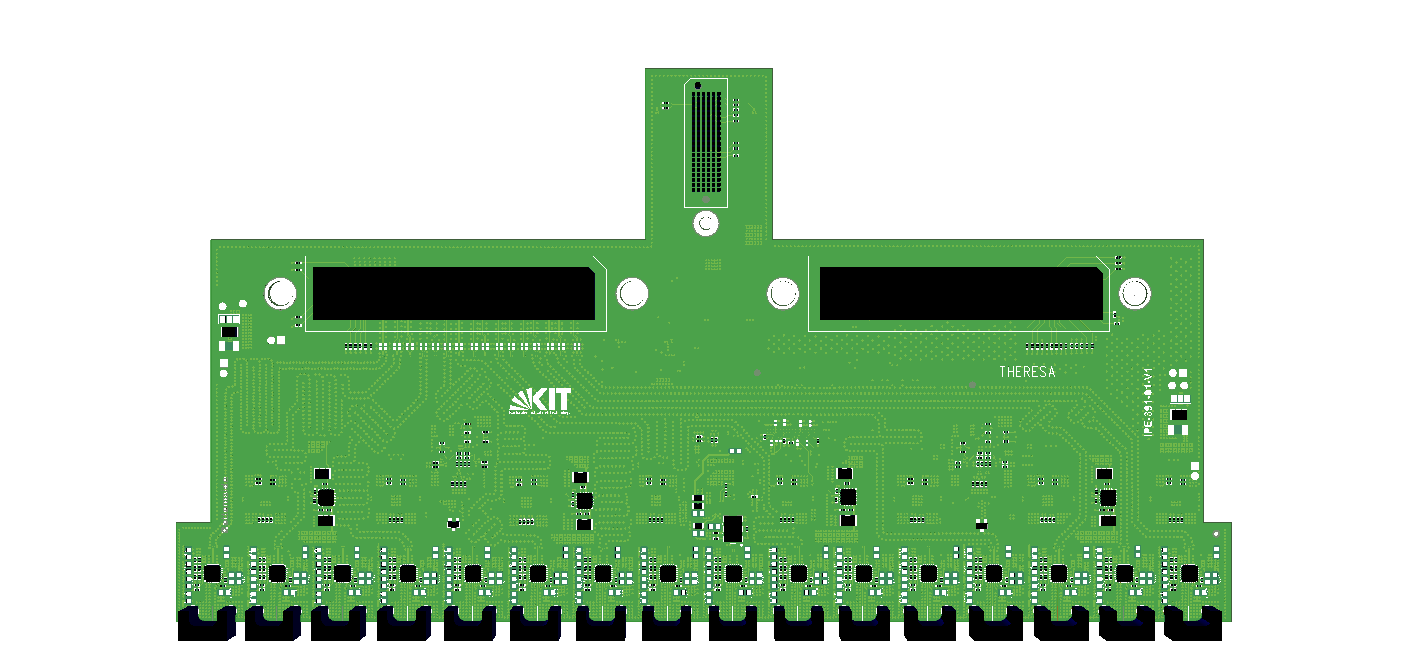
\includegraphics[width=\textwidth]{chap/04-theresa/img/pcb/back}  
		\caption{Bottom side}
		\label{fig:pcb_back}
	\end{subfigure}
	\caption[THERESA sampling card]{3D model of the THERESA sampling card, showing the top and bottom side of the card}
	\label{fig:sampling_card}
\end{figure}
